\documentclass[12pt, a4paper,twoside,openright]{book}

\usepackage{catchfilebetweentags}
\usepackage[comma, sort&compress]{natbib}
\usepackage[english]{babel}
\usepackage{graphicx}
\usepackage{color}
\usepackage{amssymb,amsmath}
\usepackage{hhline}
\usepackage[colorlinks=true,linkcolor=blue, citecolor=blue, urlcolor=blue]{hyperref}
\usepackage[hmargin=3cm,vmargin=3cm]{geometry}
\usepackage{fancyhdr}
\usepackage{hhline}
\usepackage[nottoc]{tocbibind}
\usepackage[font=small,labelfont=bf]{caption}
\usepackage{tikz}
\usetikzlibrary{trees}

\pagestyle{fancy}
\renewcommand{\chaptermark}[1]{\markboth{#1}{}}
\renewcommand{\sectionmark}[1]{\markright{\thesection\ #1}}
\fancyhf{} \fancyhead[LE,RO]{\bfseries\thepage}
\fancyhead[LO]{\bfseries\rightmark}
\fancyhead[RE]{\bfseries\leftmark}
\fancypagestyle{plain}{\fancyhead{} \renewcommand{\headrulewidth}{0pt}}
\renewcommand{\headrulewidth}{0.5pt}
\renewcommand{\footrulewidth}{0pt}
\addtolength{\headheight}{12.pt}

\newcommand{\doctype}{chapter}
\newcommand{\paperpau}{chapter~\ref{ch:pau}}
\newcommand{\paperodds}{chapter~\ref{ch:odds}}
\newcommand{\we}{we}

\renewcommand{\topfraction}{0.85}
\renewcommand{\textfraction}{0.1}
\renewcommand{\floatpagefraction}{0.75}

\setcounter{tocdepth}{1}

\begin{document}

\begin{titlepage}
\begin{center}

\textsc{\Large Doctoral Thesis in Physics}\\[1.5cm] % Thesis type

\noindent\makebox[\linewidth]{\rule{\textwidth}{1pt}} \\[0.2cm]
{\huge \bfseries 
Precise photometric redshifts with narrow-band filters, quality cuts and their impact on the measured galaxy clustering}\\[0.2cm] % Thesis title
\noindent\makebox[\linewidth]{\rule{\textwidth}{1pt}} \\[1.5cm]

\LARGE Pol Mart\'{\i} Sanahuja \\[2.0cm]

{\Large \emph{Supervisors:}\\ Ramon Miquel Pascual\\ Enrique Fern\'andez S\'anchez}\\[2cm]
 
{\Large Universitat Aut\`onoma de Barcelona}\\[0.2cm]
{\large Institut de F\'{\i}sica d'Altes Energies}\\[0.2cm] % Research group name and department name
 
{\large Barcelona \today}\\[4cm] % Date
 
\vfill
\end{center}

\end{titlepage}

\clearpage{\pagestyle{empty}\cleardoublepage}


%----------------------------------------------------------------------------------------
%	QUOTATION PAGE
%----------------------------------------------------------------------------------------

%\pagestyle{empty} % No headers or footers for the following pages

\chapter*{}

\textit{``Simplicity is the ultimate sophistication."}

\begin{flushright}
Leonardo da Vinci
\end{flushright}

\clearpage{\pagestyle{empty}\cleardoublepage}


\chapter*{Acknowledgements}
\addcontentsline{toc}{chapter}{Acknowledgements}
Many thanks to:
\begin{itemize}
\item Ramon Miquel for accepting to be my thesis adviser;

\item Enrique Fern\'andez for accepting to be my thesis co-adviser;

\item the members of the thesis committee for their time;

\item my office mates, Carles S\'anchez and Llu\'{\i}s Galbany, for joining me during this time;

\item Enrique Gazta\~naga, Francisco J. Castander, Anne Bauer, Martin Eriksen, Linda \"Ostman, Ricard Casas, Jorge Carretero, Stephanie Jouvel and Laia Cardiel for their help;

\item the PAU@WHT team, for being very enjoyable;

\item my partner, Sandra Aguilera, for being patient with me;

\item and, my family and friends, for their support.
\end{itemize}

This work was partially supported by the Spanish Ministerio de Econom\'{\i}a y Com\-pe\-ti\-ti\-vi\-dad (MINECO) under projects AYA2009-13936, FPA2012-39684, and Consolider-Ingenio 2010 CSD2007-00060.

%\clearpage{\pagestyle{empty}\cleardoublepage}

\tableofcontents
\clearpage{\pagestyle{empty}\cleardoublepage}

\chapter{Introduction}
\label{cd:intro}
Since ancient times humankind has wondered about the nature of the night sky and its celestial objects, to which it always has attributed a mystical or religious character. However, with the advent of the Modern era, and in turn the scientific method, we gradually realized that the laws of nature that govern everyday phenomena also explain the celestial world. Stars are objects just like the Sun but at much greater distance, and planets are worlds like Earth, also trapped in the Sun's gravitational field. Early last century, it was thought that the Universe was basically composed of stars uniformly spread out over space, which had occupied the same place since ever. Later, astronomers realized that in fact stars were grouped into large islands called galaxies and these again were grouped forming galaxy clusters and superclusters placed between huge voids. This is known as the large-scale structure of the Universe. Moreover, these galaxies seemed to be moving away from each other the further the faster, as if the space between them was growing. This led to the undeniable conclusion that the Universe is expanding, and it had not always been like now. In fact, about 13,700 million years ago, everything should have been confined in a much smaller space that eventually expanded and evolved into the Universe we know today. This is referred to as the theory of the Big Bang, which gave birth to a new branch of Astronomy called Cosmology, studying the matter-energy content and evolution of the Universe as a whole. A brief introduction to the astronomical and cosmological concepts necessary to understand this work is presented in the first half of chapter~\ref{ch:framework}.

Einstein's gravitational field equations predict that the evolution of the Universe and the growth of the large-scale structure are directly related to its matter-energy content. Nowadays, by measuring the evolution of the 3D position of a large number of distant galaxies, together with other cosmological probes cosmologists have determined that only about five percent of the content of the universe is ordinary matter (molecules, atoms, plasma, neutrinos and photons ) while the rest should be in two types of matter-energy whose origin and properties are unknown; Dark Matter and Dark Energy. This presents a challenge for modern Cosmology. There are several theories that attempt to respond to it, however many more galaxy surveys are needed to reach the necessary precision to rule out or confirm some of them. Spectroscopic surveys~(2dF, \citet{Colless2001}; VVDS, \citet{LeFevre2005}; WiggleZ, \citet{Drinkwater2010}; BOSS, \citet{Dawson2013}) provide a 3D image of the galaxy distribution in the near universe, but most of them suffer from limited depth, incompleteness and selection effects. Imaging surveys~(SDSS, \citet{York2000}; PanSTARRS, \citet{kaiser2000}; LSST, \citet{Tyson2003}; DES, \citet{}) solve these problems but, on the other hand, do not provide a true 3D picture of the universe, due to their limited resolution in the position along the line of sight, which is obtained measuring the galaxy redshift through photometric techniques using a set of broad-band filters, a technique known as photometric redshift (photo-$z$). The Physics of the Accelerated Universe (PAU) survey at the William Herschel Telescope (WHT) in the Roque de los Muchachos Observatory (ORM) in the Canary island of La Palma (Spain) will use narrow-band filters to try to achieve a quasi-spectroscopic precision in the redshift determination that will allow it to map the large-scale structure of the universe in 3D using photometric techniques, overcoming the limitations of spectroscopic surveys~\citep{Benitez2009}. A detailed explanation of photo-$z$ methods and an overview of the galaxy redshift surveys used in this work are given in the second half of chapter~\ref{ch:framework}.

The photo-$z$ performance capabilities of a narrow-band filter system, like that of the PAU@WHT survey, constitute the main topic of this thesis and are detailed in chapter~\ref{ch:pau}. The stringent photo-$z$ precision requirements of this survey, defined in \citet{Gaztanaga2012}, can only be achieved by applying photo-$z$ quality cuts, that is, by not considering galaxies with unreliable photo-$z$ estimations. However, if these galaxies are not removed homogeneously over the sky, this can severely bias the large-scale structure measurements. Since photo-$z$s depend mainly on the photometry whose quality depends on the atmospheric conditions of the observed region of the sky, the distribution of the photo-$z$ quality over it will not be homogeneous. Therefore, one must be careful when applying this kind of cuts. In chapter~\ref{ch:odds} we study the impact of these cuts on the angular clustering of a real luminous red galaxy based catalog \citep{Collister2007} from the Sloan Digital Sky Survey (SDSS) and propose a method to correct for it. 

Finally, in chapter~\ref{ch:conclusions}, we conclude the thesis with a brief summary of the two previous chapters, how they relate to each other, and providing a first look at their implications and possible future studies. 


\chapter{Framework}
\label{ch:framework}
In this chapter we introduce the concepts and tools necessary to follow the next two chapters. The outline is as follows. In section~\ref{sec:cosmo_model} we present the $\Lambda$CDM cosmological model, the main probes supporting it, the concepts of cosmological redshift and distances, and a brief introduction to the inhomogeneous Universe. In section~\ref{sec:photometry} we give basic notions underlying the science of photometry such as: fluxes, apparent and absolute magnitudes, photometric systems, etc. In section~\ref{sec:theo_photoz} we introduce the concept of photometric redshift, the main topic of this thesis, we explain its origin and usefulness on observational cosmology and enumerate different methods to compute it, emphasizing the BPZ method \citep{Benitez2000} used in this thesis. Finally, in section \ref{sec:surveys} we present the three galaxy redshift surveys whose data are used in this thesis, when it is available (SDSS and 2dFGRS), or simulated, when it is not (PAU@WHT Survey).

\section{Modern cosmology}
\label{sec:cosmo_model}

Modern cosmology, or simply cosmology, is the study of the largest-scale structures and dynamics of the Universe as a whole and is concerned with fundamental questions about its formation, evolution, and ultimate fate. Cosmology as a science originated with the Copernican principle, which states that celestial bodies obey identical physical laws to those on Earth. During the 20th century, Cosmology developed widely with Albert Einstein's General Theory of Relativity, and with better astronomical observations of extremely distant objects. Currently, the most accepted cosmological model is called $\Lambda$ Cold Dark Matter ($\Lambda$CDM).

\subsection{The geometry of the Universe}
The cosmological principle asserts that the distribution of matter-energy in the universe at large scales ($\gtrsim$100Mpc) is homogeneous and isotropic, so there is no preferred direction on the sky. According to the General Theory of Relativity, the unique metric compatible with this principle is the Friedmann-Lemaitre-Robertson-Walker (FLRW) metric, whose space-time line element is:  
\begin{equation}
ds^2 = -c^2dt^2 + a(t)^2dx^2,
\label{eq:space-time_line}
\end{equation}
where $-cdt$ is the temporal contribution with $c$ the speed of light and $a(t)dx$ the spatial, which is the product of a time-dependent scale factor $a(t)$ and a comoving space line element $dx$. Since only the product $a(t)dx$ has a physical meaning of distance, the absolute value of $a$ is arbitrary and it is usually taken equal to 1 today. If the scale factor grows in time ($\dot{a}>0$), spatial distances will grow as well, so in that case, we will say that the Universe is expanding. The FLRW metric admits three different kinds of spatial curvature for the whole Universe: hyperbolic, flat and spherical. In the case that it is flat, which seems to be in good agreement with the current Cosmic Microwaves Background (CMB) radiation observations~\citep{komatsu2009, Ade2013}, it can be written in spherical coordinates $\lbrace r, \theta, \varphi \rbrace$ as:
\begin{equation}
dx^2 \equiv dr^2 + r^2d\Omega^2,
\end{equation}
where $d\Omega^2 \equiv d\theta^2 + \sin^2\theta d\varphi^2$ is the differential solid angle. From now on, we will consider that the Universe is spatially flat and all equations we will show will be valid under this assumption.

\subsection{Cosmological Redshift}
When light (or any electromagnetic radiation) coming from a distant celestial object, such as a galaxy, travels across the space of an expanding Universe, all its wavelengths suffer an elongation due to the growth of distances. This effect is called cosmological redshift and it is equivalent to the elongation of the wavelengths that any wave suffers when it comes from a source which is moving away (Doppler effect). It can be quantified as: 
\begin{equation}
z \equiv {\lambda_{obs} - \lambda_{em} \over \lambda_{em}},
\label{redshift}
\end{equation} 
where $\lambda_{obs}$ is the wavelength of the light when is received by the observer and $\lambda_{em}$ when it was emitted by the source. From now on, we will simply refer to redshift when we actually refer to cosmological redshift. It is easy to show through the geodesic equation (movement equation) in a FLRW metric that there is a relation between the scale factor $a$ at the time when light was emitted and how redshifted the light is today. 
\begin{equation}
1 + z = {1 \over a(t)}
\label{z2a}
\end{equation} 
In Fig.~\ref{fig:sdss_filt} we show the spectrum of the star Vega ($\alpha$-Lyr) as reference at three different redshifts: 0, 0.4, 0.8 (note that such redshifts for a star in the Milky Way are not real, but only illustrative). As it is redshifted, its spectral features, such as the prominent absorption valleys, shift towards higher (redder) wavelength and are stretched.
\begin{figure}
\centering
\includegraphics[width=110mm]{./plots/plot_sdss_filters.png}
\caption{On the foreground, the spectrum of the star Vega ($\alpha$-Lyr) as a reference at three different redshifts: 0 (blue), 0.4 (green) and 0.8 (red). As it is redshifted, its spectral features, such as the prominent absorption valleys, move towards higher wavelength and they are stretched. The spectra have been normalized to have the same height. On the background, the throughput $R(\lambda)$ of the SDSS broad-band photometric system $ugriz$ \citep{Fukugita1996}. (Plot generated with the public script at \url{http://www.astroml.org/sklearn_tutorial/_downloads/plot_sdss_filters.py}.)}
\label{fig:sdss_filt}
\end{figure}

\subsection{The evolution of the universe}
Assuming that the matter-energy content of the universe at large scales can be described as a perfect fluid, which follows the state equation $P = \omega \rho$, where $P$ is the pressure, $\rho$ the density and $\omega$ is the state parameter of the fluid that relates them, the gravitational field equations give us the temporal evolution $a(t)$ of the FLRW metric in its differential form called the Friedman equation:
\begin{equation}
H \equiv {\dot{a} \over a} = H_0\sqrt{\sum_\omega \Omega_{\omega}a^{-3(1+w)}},
\label{eq:friedman}
\end{equation} 
where $H_0 \sim 70 (km/s)/Mpc$ is the Hubble constant, which is the value of the so called Hubble parameter $H$ today. The sum inside the root is over all the different perfect fluids that fill the universe, such as non-relativistic matter (dust, gas, cold dark matter\footnote{Cold dark matter (or CDM) is a hypothetical form of matter that interacts very weakly with electromagnetic radiation (dark) and most of whose particles move slowly compared to the speed of light (cold). Its presence can be only detected through its gravitational or weak interactions with ordinary matter and radiation.}) ($\omega \sim 0$), radiation ($\omega=1/3$), etc., and $\Omega_\omega \equiv \rho / \rho_c$ are their densities relative to the critical density $\rho_c \equiv 3H^2_0 / 8\pi G$ today, where $G\sim6.67\cdot10^{-11}N\cdot(m/kg)^2$ is the gravitational constant. Relative densities must fulfill $\sum_\omega \Omega_\omega =1$ in a flat Universe. We refer to the collection of parameters $\lbrace \Omega_\omega, H_0 \rbrace$ as the cosmology of the Universe, which determines the evolution and destiny of its space-time metric. Using the spatial part of the FLRW space-time line element at (\ref{eq:space-time_line}) and the definition of $H$, it can be deduced that the receding velocity $v$ of a galaxy in an expanding universe ($\dot{a}>0$) is $v = Hd$, where $d$ is the physical distance to the galaxy. Edwin Hubble proved, by plotting the measurements of the distance and the receding velocity of 22 galaxies (see Fig.~\ref{fig:hubble_diagram}), that this is the case for our Universe \citep{Hubble1929}. Very often cosmological parameters are given in terms of the normalized Hubble parameter $h\equiv H_0/100(km/s)/Mpc\sim0.7$. Also note that when $c>Hd$, where $c$ is the speed of light, the receding galaxy becomes causally disconnected from the observer, which defines a causal horizon.
\begin{figure}
\centering
\includegraphics[width=110mm]{./plots/Hubblediagram.pdf}
\caption{Original scatter plot from \citet{Hubble1929} of the velocity $v$ (km/s) vs. distance $d$ (pc) of 22 galaxies that proves that the universe is expanding. According to this, galaxies follow a linear relation $v=Hd$.} 
\label{fig:hubble_diagram}
\end{figure}

Besides the expansion rate of the universe given by $H$, another interesting quantity is the deceleration parameter $q$ defined as:
\begin{equation}
q \equiv -{\ddot{a} \over aH} = {1 \over 2} \sum_\omega \Omega_{\omega}{(1+3w)}.
\label{eq:deceleration}
\end{equation} 
According to this definition, a universe basically made of ordinary matter ($\omega \sim 0$) would have a deceleration parameter $>0$, that is, the expansion rate would be decelerating due to the gravitational attraction. However, any unknown component with $\omega < -1/3$ would do the opposite, accelerate the expansion rate. In the next subsection, we will see that the universe actually has a component that accelerates its expansion.

\subsection{Cosmological distances}
\label{sec:distances}
The radial comoving distance $r$ that light traveled since it left the source until it arrives to us can be computed by equating the space-time line element in (\ref{eq:space-time_line}) to 0. Note that in spherical coordinates light only travels radially respect to us ($d\Omega = 0$ and $dx = dr$). Using the definition of the Hubble parameter in (\ref{eq:friedman}) and the relation between the redshift and the scale factor in (\ref{z2a}), $r$ can be expressed as 
\begin{equation}
r(z) = c \int_0^{z} {dz' \over H(z')},
\label{comoving_distance}
\end{equation}
where the integral goes from redshift 0, when light is observed, to redshift $z$, when it was emitted. If we want to know the equivalent current physical distance, we only have to multiply by the scale factor today.

In astronomy, distances to celestial objects have been usually determined by measuring either their apparent brightness (flux $F$) on the sky when their absolute luminosities $L$ are well-known (standard candles), or their apparent sizes (angle subtended $\theta$) on the sky when their actual sizes $\ell$ are also well-known (standard rulers). It is easy to see through geometrical and energy conservation arguments that the luminosity distance to an object defined by the first equality below is related to the redshift $z$ by the second equality 
\begin{equation}
D_L \equiv \sqrt{L \over 4 \pi F}  = r(z) (1+z).
\label{eq:DL}
\end{equation}
Likewise for the angular distance:
\begin{equation}
D_A \equiv {\ell \over \theta} = {r(z) \over (1+z)}.
\label{eq:DA}
\end{equation}
These two relations are very important because they allow us to constrain the cosmology of our Universe by simply measuring the relation of a physical quantity, such as the flux $F$ or subtended angle $\theta$ of standard candles or rulers respectively, with the redshift $z$. Moreover, if we have enough redshift precision, we will be able to measure the radial size (the difference in redshift $\delta z$ between the nearest and the farthest part) of a standard ruler that is aligned with the line of sight. With this, we see by differentiating (\ref{comoving_distance}) that we can directly measure the Hubble parameter as $H(z) = c \delta z / \ell$. If the standard ruler is perfectly spherical with diameter $\ell$, we can measure $D_V(z)$~\citep{Eisenstein2005}, a hybrid distance that takes into account both contributions:
\begin{equation}
D_V \equiv \left((1+z)^2 D_A^2 {cz \over H(z)} \right)^{1/3}.
\label{eq:DV}
\end{equation}

Typical standard candles in observational cosmology are type Ia Supernovae (SNIa), which are very energetic nuclear explosions that occur when a white dwarf star in a binary system accreats material from the companion until its mass surpasses the Chandrasekhar's limit. When they are produced in another galaxy, they can shine brighter than the host galaxy itself, so they can be seen at very large distances (or very high redshifts). Moreover, after some corrections, they all appear to have very similar absolute luminosities. In the late 1990’s two independent teams, the Supernova Cosmology Project~\citep{Perlmutter1999} and the High-$z$ SN Search~\citep{Riess1998} measured the relation between the luminosity distances $D_L$ of high-$z$ SNIa ($z>0.15$) and their redshift (see Fig.~\ref{fig:hubble_diagram_sn1a}). They found that (\ref{eq:DL}) fits best the data when the cosmology is $\lbrace \Omega_{CDM} \sim 0.3, \Omega_\Lambda \sim 0.7 \rbrace$, where $\Lambda$ is an unknown component of the universe, such as a cosmological constant or dark energy, the latter with state parameter $\omega_\Lambda \sim -1$. According to this result the deceleration parameter $q$ defined in (\ref{eq:deceleration}) is negative, so the universe expansion rate is not decelerating, as was originally thought, but accelerating.
\begin{figure}
\centering
\includegraphics[width=90mm]{./plots/perlmutter_riess_hubble_diagram.pdf}
\caption{Top: The scatter plot of the distance modulus, defined in subsection~\ref{sec:absolute_mag} as $m-M \equiv 5\log_{10}(D_L / 10pc)$, vs. the redshift of low-$z$ SNIa ($z<0.15$) from the Calan/Tololo SN Search \citep{Hamuy1993} and other SN surveys, and high-$z$ SNIa ($z>0.15$) from the High-$z$ SN Search~\citep{Riess1998} and the Supernova Cosmology Project~\citep{Perlmutter1999}. Bottom: The residuals of the distances relative to a $\Omega_{CDM}=0.3$, $\Omega_\Lambda=0.0$ Universe. The best fit to data occurs with $\Omega_{CDM}=0.3$ and $\Omega_\Lambda=0.7$, which implies that the Universe expansion rate is accelerating. Figure from \citet{Perlmutter2003}.}
\label{fig:hubble_diagram_sn1a}
\end{figure}

A typical standard ruler in observational cosmology is the Baryon Acoustic Oscillation (BAO) scale. Back ($z>1100$) when the Universe was denser and hotter ($T\gg13.6$~eV) enough that hydrogen atoms could not form, the photons in the plasma of baryons and electrons continuously interacted through Thomson scattering ($p+e^- \rightleftharpoons H+\gamma$), creating a pressure on that medium through which acoustic waves traveled at the speed of sound $c_s = \sqrt{\partial p /\partial \rho}=c/\sqrt{3(1+R)}$, where $R \equiv 3\rho_b / 4\rho_\gamma$ and, $\rho_b$ and $\rho_\gamma$ are the densities of baryons and photons respectively at that time. The Universe expanded and cooled down until the recombination era when hydrogen atoms could start to form ($p+e^- \Rightarrow H+\gamma$), so the pressure on the medium vanished and traveling waves stalled at a comoving distance
\begin{equation}
r_d \sim c_s \int_{1100}^{\infty} {dz \over H(z)} \sim 150\ \rm Mpc
\end{equation}
from the initial overdensity where they were created, where $\infty$ denotes the beginning of the Universe. Additionally, photons started to move freely across space creating what we now observe as the Cosmic Microwaves Background (CMB) radiation. Recent accurate measurements of the CMB with the Plank mission show that, in fact, $r_d=147.49 \pm 0.59$Mpc at $z_d = 1059.25\pm0.58$ \citep{Ade2013}. Later, these secondary overdensities, as well as the initial ones, seeded the formation of galaxies resulting in an excess of galaxies separated by $\sim150$~Mpc from each other. \citet{Eisenstein2005} was the first to detect this preferred distance by measuring the 3D redshift-space correlation function $\xi(s)$ (black points in Fig.~\ref{fig:xi_bao}) with the SDSS survey (see subsection~\ref{sec:sdss}) LRG\footnote{Luminous Red Galaxies (LRGs) are luminous intrinsically red galaxies consistent with large/giant elliptical galaxies.} spectroscopic galaxy sample. Note, from Fig.~\ref{fig:xi_bao}, that besides the exponential decreasing shape of $\xi(s)$ there is a small bump at $\sim150$~Mpc corresponding to the BAO signature.
\begin{figure}
\centering
\includegraphics[height=90mm]{./plots/bao_eisenstein.pdf} 
\caption{The large-scale redshift-space correlation function $\xi(s)$ of the SDSS LRG spectroscopic sample \citep{Eisenstein2005}. Note that the vertical axis mixes logarithmic and linear scales. The inset shows an expanded view with a linear vertical axis. Points correspond to measured data, while lines correspond to different models. The BAO peak is clearly seen at 100~Mpc/h $\sim$ 150~Mpc. The magenta line is a model which does not include the BAO signature.}
\label{fig:xi_bao}
\end{figure}
During the last fifteen years, detections of BAO with other samples have been carried out. In Fig.~\ref{fig:DV_bao} we show a Hubble diagram $D_V$ vs. $z$ for different measurements at different redshifts with the spectroscopic samples: 2dFGRS (\citet{Colless2001}, $z=0.2$), SDSS (\citet{York2000}, $z=0.2$ and $z=0.35$) and WiggleZ (\citet{Drinkwater2010}, $z=0.6$). Two predicted curves for two different cosmologies, $\Lambda CDM\equiv\lbrace \Omega_{CDM} \sim 0.3, \Omega_\Lambda \sim 0.7 \rbrace$ (solid line) and a pure CDM Universe $\lbrace \Omega_{CDM}\sim 0.3, \Omega_\Lambda \sim 0 \rbrace$ (dashed), are also shown. Data are in agreement with the $\Lambda CDM$ model, and consistent with the SNIa results.
\begin{figure}
\centering
\includegraphics[height=75mm]{./plots/dv_bao.pdf}
\caption{The Hubble diagram $D_V(z)$, defined in (\ref{eq:DV}), vs. redshift obtained by measuring the BAO signature in a combination of the transversal and radial directions with the spectroscopic samples: 2dF (\citet{Colless2001}, $z=0.2$), SDSS (\citet{York2000}, $z=0.2$ and $z=0.35$) and WiggleZ (\citet{Drinkwater2010}, $z=0.6$). The data points agree with the prediction corresponding to a cosmology $\Lambda CDM \equiv\lbrace \Omega_{CDM} \sim 0.3, \Omega_\Lambda \sim 0.7 \rbrace$ (solid line). Figure from \citet{Astier2012}.}
\label{fig:DV_bao}
\end{figure}

Nowadays, most of the observational cosmology is focused into determining precisely the cosmology of our Universe. Current cosmological probes agree that the Universe is very close to flat and basically made of cold dark matter ($\omega_{CDM} = 0$) with relative density $\Omega_{CDM} \sim 0.3$ and some unknown ingredient called Dark Energy ($\omega_\Lambda \sim -1$) with $\Omega_\Lambda \sim 0.7$, responsible for the accelerated expansion rate. The Friedman equation for a Universe like this is reduced to:
\begin{equation}
H(z) = H_0 \sqrt{\Omega_{CDM}(1+z)^3 + \Omega_\Lambda}
\end{equation}
where $a$ on the right of equality (\ref{eq:friedman}) has been replaced by (\ref{z2a}). It is usually referred as the $\Lambda$CDM Universe. In this paradigm, ordinary matter (baryonic matter) would also account for $\lesssim5\%$ of the total content.

\subsection{Large-Scale Structure (LSS)}
\label{sec:lss}

At scales $<$100~Mpc the Universe can not be considered homogeneous since it presents structures such as galaxy clusters, voids and filaments, as shown in Fig.~\ref{fig:2dfzcone}. At those scales the FLRW metric is no longer valid however, the Newtonian description of gravity is a good approximation. Consider that small deviations at different positions and times of the density $\rho(\vec{x},t)$ of the perfect fluid can be quantified as:
\begin{equation}
\delta(\vec{x}, t) \equiv {\rho(\vec{x},t) \over \bar{\rho}(t)} - 1,
\end{equation}
which is called the density contrast, with $\bar{\rho}$ the average density. According to the Newtonian potential and mass conservation, the evolution in time of these fluctuations in an expanding universe is given by the second order harmonic differential equation:
\begin{equation}
\ddot{\delta} + 2H\dot{\delta} - {3 \over 2}H^2 \delta = 0,
\label{eq:diff_delta}
\end{equation}
where $H$ is the Hubble parameter defined in (\ref{eq:friedman}). The solution, $\delta(\vec{x},t) = D^{\pm}(t)\delta(\vec{x})$, consists of a growing ($+$) and a decaying ($-$) mode, with completely decoupled temporal and spatial parts. Since eventually the growing mode dominates, we simply write the solution as 
\begin{equation}
\delta(\vec{x},z) = D(z)\delta(\vec{x}),
\label{eq:growth_factor}
\end{equation}
where $D(z)$ ($t$ has been replaced by $z$ through (\ref{z2a})) is called the linear growth factor and gives the evolution in redshift (time) of the initial spatial perturbation $\delta(\vec{x})$.
Clearly, the evolution of these perturbations and, therefore, the evolution of the large-scale structure, is not only driven by the gravitational pull of the perturbations themselves, but also by the evolution of the space-time metric of the whole Universe. This allows cosmologists to trace the history of $a(t)$ and determine the cosmology of the Universe by observing how structures have formed and evolved.
\begin{figure}
\centering
\includegraphics[width=130mm]{./plots/2dFzcone_big.png}
\caption{The distribution of $\sim 0.2$~million galaxies (blue) observed with the 2dFGRS survey \citep{Colless2001} in two slices $4$~deg thick, centered at declination $-2.5$~deg in the North Galactic Pole and $-27.5$~deg in the South Galactic Pole. Although the distribution of matter at large scales ($>100$~Mpc) can be considered as homogeneous and isotropic, at lower scales galaxies form structures such as galaxy clusters, voids and filaments.}
\label{fig:2dfzcone}
\end{figure}
Since the formation of galaxies is seeded by cold dark matter overdensities (the most dominant component of matter), the easiest way to trace the distribution of cold dark matter is by looking at the three-dimensional position of galaxies on the sky. However, in \citet{Fry1993} it was shown that there is a bias $b$ between the fluctuations of the galaxy density contrast $\delta_G$ and the CDM density contrast $\delta$ defined as follows
\begin{equation}
\delta(\vec{x},z)_G = b(z) \delta(\vec{x},z),
\label{eq:bias}
\end{equation}
where $b$ can depend on the redshift.

Cosmologists are not actually interested in the value of $\delta(\vec{x},z)$, but in its statistical properties. For this purpose, they compute the two-point correlation function in a given volume $V$
\begin{equation}
\xi(\vec{r}) = \langle \delta(\vec{y}) \delta(\vec{y}+\vec{r}) \rangle_V = {1 \over V}\int \delta(\vec{y})\delta(\vec{y}+\vec{r})dV_y,
\end{equation}
which, assuming isotropy, gives the differential probability $dP = \bar{\rho}^2(1+\xi(r))dV_ydV_{y+r}$ to find a fluctuation of size $\delta (\vec{y})$ a distance $r=|\vec{r}|$ away from another fluctuation of size $\delta (\vec{y}+\vec{r})$. Even more interesting is the Fourier transform of the 2-point correlation function $\xi(\vec{r})$:
\begin{equation}
P(\vec{k}) = \int \xi(\vec{r})e^{i\vec{k}\vec{r}}d^3k,
\end{equation}
which is called the matter power spectrum. Note that the density contrast, $\delta({\vec{x}})$, can also be Fourier transformed to $\delta({\vec{k}})$, so that the matter power spectrum can be computed simply as $P(\vec{k})=V|\delta(\vec{k})|^2$. Most inflationary\footnote{Inflation is a cosmological model for the early universe that predicts an extremely rapid exponential expansion driven by a negative-pressure vacuum energy density. Initial quantum fluctuations become macroscopic on this process seeding the current inhomogeneities observed on the matter distribution.} theories predict a primordial density contrast whose amplitude $\delta(\vec{r})$ is isotropic and homogeneously Gaussian distributed (observationally confirmed in \citet{komatsu2009}), as well as a power spectrum $P(k) \propto k$ (Harrison-Zeldovich power spectrum) that is scale-invariant. However, the shape of $P(k)$ at low scales is strongly modified by the radiation dominated era ($\Omega_{rad} \gg \Omega_{matter}$) where perturbations whose wavelength scale $\lambda$ was smaller than the causal horizon had a linear growth factor $D(z)$ that remains constant until the matter dominated era due to the suppression caused by the pressure of radiation (see \cite{Dodelson2003} for a more detailed explanation). This results in the power spectrum, shown in Fig.~\ref{fig:pk}, which asymptotes to $P(k)\sim k$ for small $k$, and behaves as $P(k)\sim k^{-3}$ for large $k$, with a peak at $k^\ast \sim 2 \times 10^{-2} h\ \rm Mpc^{-1}$ corresponding to $\lambda^\ast\sim 350 h^{-1}\ \rm Mpc$.
\begin{figure}
\centering
\includegraphics[width=110mm]{./plots/pk.pdf}
\caption{Matter power spectrum $P(k)$ vs.~wavenumber extrapolated to $z=0$, from various measurements of cosmological structure. The best fit $\Lambda CDM$ model is shown as a solid line. Figure from \citet{Tegmark2002b}.}
\label{fig:pk}
\end{figure}

We typically measure distances to galaxies through the relation between their redshift and distance given by the Hubble law. However, peculiar radial velocities of galaxies not associated with the expansion flow can cause distortions on the measurement of the cosmological redshift. The most obvious example of this is the Fingers-of-God effect \citep{Bahcall1986}, where long thin filaments in the distribution of galaxies in redshift space point directly back at the observer due to the addition of the random peculiar velocities of galaxies, given by the virial theorem\footnote{The virial theorem relates the average over time of the total kinetic energy of a stable system consisting of $N$ particles, bound by potential forces, with that of the total potential energy.}, in the radial direction within a galaxy cluster. Another important redshift-space distortion is the Kaiser effect \citep{Kaiser1984}, which is more subtle and difficult to quantify. The Kaiser effect describes the peculiar velocities of galaxies bound to a central mass as they undergo infall. This differs from the Fingers-of-God in that the peculiar velocities are coherent, not random, towards the central mass. According to this effect, in the large-scale linear regime ($\delta \ll 1$) and the plane-parallel approximation (where galaxies are taken to be sufficiently far away from the observer that the displacements induced by peculiar velocities are effectively parallel), the distortion caused by coherent infall velocities takes a particularly simple form in Fourier space:
\begin{equation}
\delta^s(\vec{k})=(b+f\mu^2_{\vec{k}})\delta(\vec{k}),
\label{eq:kaiser}
\end{equation}
where $\mu$ is the cosine of the angle between $\vec{k}$ and the line-of-sight, $b$ is the bias described in (\ref{eq:bias}), the subscript $s$ indicates redshift space, and $f$ is the velocity growth factor defined as
\begin{equation}
f(z)\equiv{d\ln D \over d \ln a}={\dot{\delta} \over \delta}\equiv\Omega_{CDM}^\gamma(z),
\end{equation}
and $\gamma$, the gravitational growth index \citep{Linder2008}.

In many cases what is measured is the angular galaxy-galaxy cross-correlation function of the galaxies at different redshifts. It can be predicted by considering the projected spatial galaxy contrast in a redshift bin $i$
\begin{equation}
\delta_{G_i}(\hat{n}) = \int dz N_i(z) \delta (\hat{n}, z),
\end{equation}
where $N_i(z)$ is the redshift distribution in the redshift bin $i$ and $\hat{n}$ is some unitary vector pointing to some direction on the sky. Then, the angular cross-correlation between two redshift bins $i$ and $j$ is
\begin{equation}
\omega_{G_iG_j} (\theta) \equiv \langle \delta_i (\hat{n}) \delta_j(\hat{n}+\hat{\theta}) \rangle = \int dz_1 N_i(z_1) \int dz_2 N_j(z_2) \xi^s(r_{12}),
\label{eq:corr_prediction}
\end{equation}
where $\xi^s(r_{12})$ is the redshift space correlation of the pairs of galaxies at redshift $z_1$ and $z_2$ subtending an angle $\theta$ with the observer, which is related to the redshift-space dark matter correlation function $\xi^s(r)$ through 
\begin{equation}
\xi^s(r_{12}) \equiv \langle \delta_g (\hat{n},z_1) \delta_g(\hat{n}+\hat{\theta},z_2) \rangle=b(z_1)b(z_2)D(z_1)D(z_2) \xi^s(r),
\end{equation}
where $b(z)$ is the bias at redshift $z$ described in (\ref{eq:bias}) and $D(z)$ the linear growth factor described in (\ref{eq:growth_factor}). The function $\xi^s(r)$ is obtained by inverse Fourier transforming the power spectrum $P^s(k)=V|\delta^s(k)|^2=(b+f\mu_k^2)^2P(k)$ as described in \citet{Hamilton1992}, where in the second equality we have used (\ref{eq:kaiser}).

In the case that perturbations in the perfect fluid are not small, $\delta \sim 1$, linear theory is no longer valid. Therefore, in order to study the evolution of these non-linear structures further, which are the seeds for galaxies and clusters, large numerical simulations are carried out. Starting from a Gaussian random field, a realization is evolved in time. The resulting dark matter structures can be investigated to find fitting formulas for the non-linear power spectrum, as done in \citet{Smith2003}. These non-linear structures begin to be important at $k\gtrsim0.2h\ \rm Mpc^{-1}$ in the matter power spectrum, which at typical redshifts correspond to an angular scale of $\theta \lesssim 0.1$~deg.

When two redshift bins $i$ and $j$, one in the foreground with mean redshift $z_i$ and the other on the background with mean redshift $z_j$ ($z_j > z_i$), are cross-correlated, the measured signal comes mainly from the galaxies in the overlap of these two redshift bins. However, a smaller contribution can come from the gravitational lensing effect that the foreground produces onto the background, which basically consists on changing the area and the brightness of the background sources behind the foreground lenses. This phenomenon is called weak-lensing magnification and it is characterized by inducing an extra term of fluctuations on the galaxy density contrast, $\delta_G \rightarrow \delta_G + \alpha \delta_\mu$, where $\alpha \equiv 2.5s-1$ is the amplitude of the weak lensing magnification effect (with $s \equiv d\log_{10}N(<m) / dm $, the slope of the galaxy number counts $N$ at the magnitude limit $m$ of the galaxies in the bin). This extra term generates three extra terms on the galaxy-galaxy cross-correlation, $\omega'_{G_iG_j} = \langle (\delta_{G_i} + \alpha_i \delta_{\mu_i}) (\delta_{G_j} + \alpha_j \delta_{\mu_j})\rangle = \omega_{G_iG_j} + \omega_{G_i\mu_j} + \omega_{\mu_i G_j} + \omega_{\mu_i \mu_j}$. The first one is already shown in (\ref{eq:corr_prediction}), while the other three involve weak-lensing magnification:
\begin{eqnarray}
\omega_{G_i\mu_j} (\theta) = \alpha_j \int dz_1 N_i(z_1) \int dz_2 N_j(z_2) b_i(z_1) p_{\mu_j}(z_2) \xi^s(r_{12}), \\
\omega_{\mu_iG_j} (\theta) = \alpha_i \int dz_1 N_i(z_1) \int dz_2 N_j(z_2) p_{\mu_i}(z_1) b_j(z_2) \xi^s(r_{12}), \\
\omega_{\mu_i\mu_j} (\theta) = \alpha_i \alpha_j \int dz_1 N_i(z_1) \int dz_2 N_j(z_2) p_{\mu_i}(z_1) p_{\mu_j}(z_2) \xi^s(r_{12}),
\end{eqnarray}
where we have used the relation (\ref{eq:bias}) for the bias $b(z)$, and $p_{\mu}(z)$ is the efficiency of the weak-lensing magnification effect between the two galaxy bins: 
\begin{equation}
p_{\mu_i}(z) \simeq {3\Omega_{CDM}H_0r(z) \over 2H(z)a(z)r_0}\int^\infty_z dz'{r(z';z) \over r(z')}N_i(z)
\end{equation}
where $r(z)$ is the radial comoving distance defined in (\ref{comoving_distance}), $r(z';z)$ is the angular diameter comoving distance between $z'$ and $z$, $r_0\equiv c/H_0$, and $N_i(z)$ is the redshift distribution of the galaxies in redshift bin $i$.

\section{Photometry}
\label{sec:photometry}
Photometry, in the context of astronomy, is the technique concerned with measuring the flux of an astronomical object's electromagnetic radiation over large wavelength intervals ($\sim100$nm). This is in contrast to spectroscopy in which the same electromagnetic radiation is split into small wavelength intervals ($\sim1$nm) with a chromatic disperser such as a prism. Nowadays, most of the astronomical photometry is carried out using Charge-Coupled Devices (CCDs) as detectors that count individually the number of photons coming from the celestial sources.

\subsection{Photometric system}
A photometric system is a set of well-defined passbands (or filters) with a known sensitivity to incident radiation. The first known standardized photometric system is the \texttt{UBV} photometric system \citep{Johnson1953}, widely used for star classification, which is composed of three broad bands that cover the ultraviolet (U), blue (B) and visual (V) regions of the spectrum (from $\sim$300~nm to $\sim$650~nm). At present, there are more than 200 photometric systems. One of the most famous is the $ugriz$ system \citep{Fukugita1996} used in the Sloan Digital Sky Survey (SDSS) instrument, whose five bands, shown in gray on Fig.~\ref{fig:sdss_filt}, cover from $\sim$300~nm to $\sim$1000~nm. The three bands $ugr$ are roughly equivalent to the $UBV$ ones, and the remaining three reach into the infrared range, which is very useful to detect and measure light coming from distant galaxies whose spectrum has been substantially redshifted.

Photometric systems can be classified according to the widths of their passbands as: broad band, whose passbands are wider than $\sim30$~nm, such as the \texttt{UBV} or the $ugriz$ systems, and narrow bands, whose passbands are less than $\sim30$nm wide, such as the PAU (subsection~\ref{sec:pau}) or ALHAMBRA~\citep{Moles2008} photometric systems.

\subsection{Flux and Apparent magnitude}
The flux $F$ of an astronomical object is the amount of energy as electromagnetic radiation that we receive from the object per unit area and time. If the electromagnetic radiation passes through a bandpass then the received flux is:
\begin{equation}
F = \int^{\infty}_0 f_\nu(\nu)R_\nu(\nu)d\nu = \int^{\infty}_0 f_\lambda(\lambda)R_\lambda(\lambda)d\lambda,
\label{eq:flux}
\end{equation}
where $\nu$ and $\lambda$ are the frequency and wavelength of the radiation respectively, which satisfy $\lambda \nu = c$, $f_\nu(\nu)$ and $f_\lambda(\lambda)$ are the spectral density fluxes of the object, these are the fluxes per unit frequency and wavelength respectively, and $R_\nu(\nu)$ and $R_\lambda(\lambda)$ are the transmission profiles of the bandpass as a function of frequency and wavelength respectively, which give the probability that a photon with associated frequency $\nu$ or wavelength $\lambda$ passes through the filter.

Fluxes of different astronomical objects, or even of the same object but at different passbands, can differ by several orders of magnitude between them. The logatithmic response of the human eye is well adapted to this wide range of fluxes. In fact, ancient astronomers classified stars according to how many times they seemed to shine with more intensity than other stars. This classification has persisted over time and has been formalized through: 
\begin{equation}
m \equiv -2.5\log{F \over F_0} \Longleftrightarrow F = F_0 10^{-0.4m},
\label{eq:mag}
\end{equation}
where $m$ is called the apparent magnitude of the object and $F$ is the actual flux received from it. The zero subindex indicates that the value of the apparent magnitude is defined with respect to another object with flux $F_0$, which defines the zero point. Different zero points define different magnitude systems, such as, for example, the Vega system in which the star Vega is defined to have an apparent magnitude of zero as measured through all filters (that is, $F_0$ is Vega's flux).

\subsection{The AB magnitude system}
Another widely used system is the AB magnitude system, which is not defined by flux ratios as in (\ref{eq:mag}) but spectral density flux $f_\nu(\nu)$ ratios, in such a way that
\begin{equation}
m^R_{AB} \equiv -2.5\log{ \int^{\infty}_0 f_\nu(\nu)R_\nu(\nu){d\nu \over \nu} \over \int^{\infty}_0 f^\nu_0 R_\nu(\nu) {d\nu \over \nu}} = -2.5\log{ \int^{\infty}_0 f_\lambda(\lambda)R_\lambda (\lambda)  (\lambda / c) d\lambda \over \int^{\infty}_0 f^\lambda_0 (\lambda) R_\lambda (\lambda) (\lambda / c) d\lambda},
\label{eq:magAB}
\end{equation}
where the reference flux is $f^\nu_0=3631Jy$\footnote{$1Jy = 10^{-23}erg \cdot cm^{-2} \cdot s^{-1} \cdot Hz^{-1}$  or $1.51 \cdot 10^7 \cdot photons \cdot m^{-2} \cdot s^{-1} \cdot dlog^{-1}\lambda$ in terms of photons.}~\citep{Oke1983}, which is constant in terms of frequency $\nu$, or $f^\lambda_0 (\lambda) = (c/\lambda^2) f^\nu_0$, which depends on $\lambda$, $c$ being the speed of light. In the second equality we have used the relations $\nu \lambda =c$, $d\nu / \nu = -d\lambda / \lambda$ and $\nu f(\nu) = \lambda f(\lambda)$. In the AB magnitude system a source with constant flux per unit frequency will have the same magnitude value in all bands. If we consider a bandpass infinitely narrow such that $R(\nu) \rightarrow \delta(\nu)$, the previous definition becomes
\begin{equation}
m_{AB}(\nu) = -2.5 \log f(\nu) - 48.6.
\end{equation}

\subsection{Color index}
In the same way that magnitudes quantify how brighter is a celestial object with respect to another, the color index quantifies how bluer or redder it is. It is defined as the difference between the magnitude $m_a$ of the celestial object in one passband $a$ with mean wavelength $\lambda_a$ and the magnitude $m_b$ of the same celestial object in a different passband $b$ with mean wavelength $\lambda_b$ such that $\lambda_a<\lambda_b$. According to the magnitude definition in (\ref{eq:mag}), if $m_a-m_b<0$, the ratio of fluxes between the celestial object $F$ and the object of reference $F_0$ in the two different bands fulfill $(F/F_0)_a>(F/F_0)_b$, so that more flux is coming from the bluer part of the object's spectrum with respect to the reference spectrum and, therefore, the object is bluer than the reference. For example, in the Vega photometric system, the Vega star has $m_V = m_B = 0$, so obviously its color index is $B-V \equiv m_B-m_V = 0$. Therefore, a star with $B-V<0$ is bluer than Vega while a star with $B-V>0$ is redder. 

Color indices are very useful in galaxy surveys to classify galaxies according to their color, which, in a similar way as stars, tell us about its activity, temperature and age. For example, red galaxies, also known as early-type galaxies or ellipticals, are older, with less star-formation activity and with a higher metalicity than bluer ones, which are known as late-type galaxies or starburst galaxies.

\subsection{Absolute magnitude and K-correction}
\label{sec:absolute_mag}
The absolute magnitude $M$ is defined to be the apparent magnitude that a source would have if it were 10 pc away, at rest (i.e., not blue- or red-shifted), and compact. In \citet{Hogg1996} it is shown that its relation with the apparent magnitude is:
\begin{equation}
M = m - \mu - K,
\end{equation}
where $\mu$ is the distance modulus 
\begin{equation}
\mu \equiv 5 \log \left[{D_L \over 10pc} \right],
\end{equation}
where $D_L$ is the luminosity distance, defined in (\ref{eq:DL}), to the source in parsecs, and the last term the $K$-correction 
\begin{equation}
K \equiv -2.5 \log \left[{1 \over 1+z}{\int^{\infty}_{0} f_\lambda \left( \lambda / 1+z \right)R(\lambda)\lambda d\lambda \over f_\lambda(\lambda)R(\lambda)\lambda d\lambda}\right], 
\end{equation}
which corrects for the fact that in an expanding universe the spectrum $f(\lambda)$ of a source at a certain distance is redshifted by $1+z$ (so that $f(\lambda) \rightarrow f(\lambda/1+z)$ according to (\ref{redshift})) and therefore, the passband $R(\lambda$) does not see the same part of the spectrum.

The absolute magnitude is a measure of the celestial object's intrinsic brightness. Note that the distance modulus $\mu = m - M - K$ only depends on the redshift $z$ and the profile of the object's spectrum $f_\lambda(\lambda)$ for a given cosmology $\lbrace \Omega_\omega, H_0 \rbrace$. This is specially useful to constrain cosmology with standard candles such as SNIa (section~\ref{sec:distances}), since their absolute magnitude is known beforehand.

\subsection{Luminosity function}
A quantity closely related to the absolute magnitude $M$ is the Luminosity Function (LF), which is the cumulative distribution of stars or galaxies up to a certain luminosity $L$ (energy per unit time). The Schechter function~\citep{Schechter1976} provides a parametric description of the LF, which in differential form is
\begin{eqnarray}
n(x)dx &=& \phi x^\alpha e^{-x}dx, \\
\mbox{with}\ x &\equiv& {L \over L^*}.
\end{eqnarray}
Since $L \propto F \propto 10^{-0.4M}$ we can write $x$ in terms of the absolute magnitude, $x = 10^{-0.4(M-M^*)}$. The function is parametrized by $\lbrace \phi, \alpha, M^*  \rbrace$, where $\phi$ has units of number density and provides the normalization, $\alpha$ is the power-law slope at high magnitudes and $M^*$ the characteristic absolute magnitude where the power-law profile cuts off.

The galaxy LF may have different parameters for different populations and environments; it is not a universal function. In Figs.~\ref{fig:LF_type} and \ref{fig:LF_redshift} we show examples of LF in the $U$-band calibrated with data from the Hubble Space Telescope (HST) and the Great Observatories Origins Deep Survey (GOODS) \citep{Dahlen2005}. They will be used in chapter~\ref{ch:pau} in order to create galaxy mock catalogs for the PAU survey (subsection \ref{sec:pau}). While in Fig.~\ref{fig:LF_type} galaxies have been grouped in different spectral types such as early-type (Ellipticals), late-type and starburst (spirals and irregulars) galaxies, in Fig.~\ref{fig:LF_redshift} we show the evolution in redshift of the composite (LF) through three different $z$-bins: $0.1<z<0.5$, $0.5<z<0.75$ and $0.75<z<1.0$.
\begin{figure}
\centering
\includegraphics[width=130mm]{./plots/LF_type.pdf}
\caption{Left: Rest-frame U-band luminosity function in the redshift range $0.1<z<0.5$, showing the composite LF (black circles) and the type-specific LFs for early-type (red circles), late-type (green circles), and starburst (blue circles) galaxies. The types are determined from best-fitting spectral templates. Right: The 68.3\% and 95\% error ellipses for $M^*$and $\alpha$ from Schechter function fits to different populations. Figures from \citet{Dahlen2005}.}
\label{fig:LF_type}
\end{figure}

\begin{figure}
\centering
\includegraphics[width=130mm]{./plots/LF_redshift.pdf}
\caption{Rest-frame U-band luminosity function for the redshift intervals $0.1 < z < 0.5$ (left), $0.5 < z < 0.75$ (middle), and $0.75 < z < 1.0$ (right). Solid red lines show the best-fit Schechter function, while dashed black lines show the best-fitting Schechter function for which the faint-end slope, $\alpha$, is fixed to the value measured in the lowest redshift bin. For comparison, we show with a gray line in the mid- and high-redshift bins the best-fitting Schechter function found in the low-redshift bin. Figures from \citet{Dahlen2005}.}
\label{fig:LF_redshift}
\end{figure}
\subsection{Measuring magnitudes}
\label{sec:measuring_mag}
We mentioned that photometry is a technique concerned with measuring the flux of an astronomical object's electromagnetic radiation. In fact, astronomers do not measure fluxes directly, but the number of incident photons $N_{obj}$ that the telescope collects in a certain period of time. These photons are detected and counted by a CCD (Charge-Coupled Device) imaging camera. CCDs were invented in 1969 at AT\&T Bell Labs by Willard Boyle and George E. Smith (Nobel Laureates in Physics in 2009), and rapidly began to be widely used for imaging. A CCD is a two-dimensional matrix of pixels that convert infalling photons into electric charge through the photo-electric effect. Then, by applying weak electrical fields, one can move this charge throughout the pixels until it reaches the edge of the matrix where the cumulated charge is measured and digitalized. In observational astronomy, the Focal Plane (FP) of the telescope where the images of the objects are formed, is covered with several CCDs.  Usually the image of a celestial object covers several pixels, even if it is a point source such as a star or a quasar. The focal plane scale $\alpha$ translates the angular size of a portion of the sky to the number of pixels the image occupies. The integrated flux of the source can be computed directly by summing up the photon counts in a certain region over the FP that encloses the object image, as shown with the green circles in Fig.~\ref{fig:sextractor}. However, often it is difficult to know where the limits of the object are, so on those cases more sophisticated ways are used, such as integrating a model for the 2D-image profile whose parameters are obtained by fitting it previously to the image. 
\begin{figure}
\centering
\includegraphics[width=90mm]{./plots/sun226fig.png}
\caption{Illustration of how a software for source extraction, such as the \texttt{SExtractor}~\citep{Bertin1996}, detects galaxies from an image and selects an effective area (green circles) around them where the flux will be integrated.}
\label{fig:sextractor}
\end{figure}
Focusing on the photometry of the SDSS survey (subsection~\ref{sec:sdss}), which will be used in chapter~\ref{ch:odds}, and depending on how they are measured, several magnitudes are defined:
\begin{itemize}

\item \textbf{PSF magnitudes:} For ground based optical telescopes, point source targets, such as stars or quasars, appear on the FP with a certain size due to aberrations introduced by atmospheric turbulence (seeing), diffraction caused by the optics, etc. On those cases, the 2D distribution of light of the image is well described by the Point Spread Function (PSF), which usually would be an Airy pattern from diffraction theory. However, in most cases it can be approximated by a Gaussian profile.

\item \textbf{Model magnitudes:} Just as the PSF magnitudes are optimal measures of the fluxes of stars, the optimal measure of the flux of a galaxy would use a matched galaxy model. Typically, two models are fitted to the 2D image of each object: a pure De Vaucoleurs profile~\citep{vaucouleurs48}
\begin{equation}
I(r)=I_0 e^{-7.67({r/r_e})^{1/4}},
\end{equation}
and a pure exponential profile 
\begin{equation}
I(r)=I_0 e^{-1.68(r/r_e)},
\end{equation}
where $I(r)$ is the brightness at a distance $r$ from the center of the image, $I_0$ is the brightness at the center and $r_e$ an effective radius. The model magnitudes in all the bands will be computed by applying the model (exponential or De Vaucouleurs) of higher likelihood in some reference band filter (the $r$-band in SDSS) and then the same model with the same $r_e$ to the rest of the bands, allowing only the amplitude to vary. This procedure ensures that the color index between different bands is measured through a consistent aperture.

\item \textbf{De Vaucouleurs magnitudes:} The De Vaucouleurs profile is specially good to describe the brightness of elliptical galaxies, therefore the best estimate of the magnitudes for these kind of galaxies is obtained by fitting a pure De Vaucouleurs profile to their image in each band independently. The value of the $r_e$ parameter in some band is called the De Vaucoleurs radius in that band, and is specially useful for galaxy-star separation in catalogs of elliptical galaxies, since they present a $r_e$ value substantially larger than stars. 

\item \textbf{Petrosian}, \textbf{Fiber}, \textbf{Detmodel}, \textbf{Cmodel}, \textbf{Aperture}, \textbf{Auto magnitudes} and many others whose importance is beyond the scope of this work. 

\end{itemize}

Once the counts of photons of the celestial object $N_{obj}$ are estimated, the value of the magnitude is given by Eq.~(\ref{eq:mag}) replacing $F$ by $N_{obj}$ and $F_0$ by the number of counts of the reference object (when observed in the same conditions, i.e. same exposure time). We can also estimate the error of the magnitude as $\sigma_m = |(m \pm \sigma_m) - m| = |- 2.5\log_{10}(F\pm \sigma_F) + 2.5\log_{10}(F)| = |2.5\log_{10}(1 \pm \sigma_F/F)|$, 
where if $F\gg\sigma_F$ then the two solutions are approximately the same. Defining the signal-to-noise (S/N) ratio as the inverse of $\sigma_F/F$, we have that:
\begin{equation}
\sigma_m = 2.5\log_{10}\left(1+{1\over(S/N)}\right).
\end{equation}
The noise, for ground based telescopes, is basically given by adding quadratically three components: the Poisson noise of the signal coming from the object $\sqrt{N_{obj}}$, the Poisson noise of the signal coming from the intrinsic sky brightness $\sqrt{N_{sky}}$ (which is integrated within the same area of the object's image) and the Gaussian noise $RN$ introduced by the electronics in the read-out system. The resulting signal-to-noise ratio expression is:
\begin{equation}
{S \over N} = {N_{obj}\over \sqrt{N_{obj}+N_{sky}+RN^2}}.
\end{equation}

Besides photometric distortions introduced on the measured flux of a celestial object by the Earth's atmosphere (e.g.~the sky brightness and atmospheric absorption) and by the optics of the telescope+camera system, galactic gas and dust between an astronomical object and the observer also absorb and scatter part of the electromagnetic radiation. Since bluer light is more strongly attenuated than redder, dust extinction causes objects to appear redder than expected, a phenomenon referred to as reddening (not to be confused with redshift). In order to measure magnitudes properly, they must be corrected for galactic (Milky way) extinction in each band. In any photometric system, interstellar reddening can be described by a color index excess, defined as the difference between an object's color index and its intrinsic color index (the color index it would have if it was not affected by extinction).

\section{Photometric Redshifts (Photo-$z$s)}
\label{sec:theo_photoz}

A photometric redshift (photo-$z$) is an estimate for the redshift of an astronomical object, such as a galaxy or quasar, using its photometry $m_i$ in various standard filters $i$. This is in contrast to the spectroscopic redshift (spec-$z$) where the shift in a spectral feature, such as an emission or absorption line, along the spectrum is determined, allowing the determination of $z$ directly from its definition in (\ref{redshift}). 

The technique is an old idea that originated in the 1960s (\citet{Baum1962, Puschell1982, Koo1985, Loh1986, Connolly1995}), but was later largely replaced by spec-$z$s. However, it has made a come-back in the last two decades, as a result of new large sky surveys (section \ref{sec:surveys}), since it provides galaxy redshifts substantially faster than the spectroscopic technique, especially when the observed objects are faint. Moreover, photo-$z$ based surveys do not suffer the incompleteness of the target selection needed in spectroscopic surveys, since all objects in the telescope's field-of-view are registered at once (in contrast to spectroscopic surveys where the spectrograph must be pointed to each target individually and some objects may be ignored). The disadvantage is that the precision for these sorts of measurements is typically $\sigma_z \sim 0.05-0.10$, and are less reliable than spectroscopic determinations.  

There are basically two types of methods to determine photometric redshifts: the template-fitting methods (e.g. Hyperz, \citet{Bolzonella2000}; BPZ, \citet{Benitez2000} \& \citet{Coe2006}; LePhare, \citet{Ilbert2006}; EAZY, \citet{Brammer2008}; LRT, \citet{Assef2008}; GALEV and GAZELLE, \citet{Kotulla2008}), and the training-set methods (e.g. ANNz, \citet{Collister2004}; ArborZ, \citet{Gerdes2010}; TPZ, \citet{CarrascoKind2013};  Li, \citet{Li2008}; Carliles, \citet{Carliles2010}). In some cases a method can belong to the two previous groups at the same time (e.g. Kernelz; \citet{Wolf2014}), so they are called hybrid methods. In this thesis we will focus on the template-fitting methods leaving the training-set and hybrid methods as alternatives. 

In order to calibrate the goodness of the photo-$z$ determinations one typically uses a spectroscopic sample with known spec-$z$ redshifts, taken as fiducial. In Fig.~\ref{fig:phat_photoz} we show several scatter plots of $\Delta z \equiv z_{ph} - z_{sp}$ vs. $z_{sp}$, where $z_{ph}$ is the photometric redshift and $z_{sp}$ the spectroscopic one, for different photo-$z$ methods applied on the same galaxy sample. If the photo-$z$ determination was perfect, all the points would be at $\Delta z = 0$ (over the black line). However, they are actually spread out around this value. The problem is that they are not typically spread out according to a Gaussian profile, but rather to a more complex distribution with asymmetries, bias, double maxima, etc., which needs to be characterized carefully. Moreover, these $\Delta z$ distributions can rapidly change their shape with redshift, spectral type, magnitude, etc. Usually, these complex distributions are characterized using three different metrics: the bias (mean, median, etc.), which tell us how the overall shape of the distribution is offset from $\Delta z =0$, the precision (RMS, $\sigma_{68}$, etc.), which tells us how dispersed are the photo-$z$ determinations from these offsets, and the outlier fraction, which tells us the rate of determinations much worse than expected (that is, the extend of the tails of the $\Delta z$ distribution).
\begin{figure}
\centering
\includegraphics[width=140mm]{./plots/phat_dzvsz.pdf}
\caption{Scatter plots $\Delta z \equiv z_{ph} - z_{sp}$ vs. $z_{sp}$, where $z_{ph}$ is the photometric redshift and $z_{sp}$ is the spectroscopic redshift, of galaxies from the Great Observatories Origins Deep Survey northern field (GOODS-N, \citet{Giavalisco2004}) in the PHAT1 test \citep{Hildebrandt2010} for different photo-$z$ methods: BPZ (BP-t or BP2-t, \citet{Benitez2000}), EASY (EA-t, \citet{Brammer2008}), GALEV and GAZELLE(GA-t, \citet{Kotulla2008}), Hyperz (HY-t, \citet{Bolzonella2000}), Kernelz (KR-t), Le Phare (LP-t, \citet{Arnouts1999} \& \citet{Ilbert2006}), LRT (LR-t, \citet{Assef2008}), ANNz (AN-e, \citet{Collister2004}), Wolf (EC-e, \citet{Wolf2014}), Li (PO-e, \citet{Li2008}) and Carliles (RT-e, \citet{Carliles2010}). Faint objects with $R\ge24$ are shown in red. Figure from \citet{Hildebrandt2010}.}
\label{fig:phat_photoz}
\end{figure}

\subsection{Template-Fitting Methods}
The template-fitting methods compare the observed fluxes $F_i$ of the celestial object in different passbands $i$ with the predicted fluxes $F_i^t(z)$ obtained by redshifting a set of spectral templates, $f^t(\lambda) \rightarrow f^t(\lambda/1+z)$, and integrating them in the passbands $R_i(\lambda)$ through Eq.~(\ref{eq:flux}). The photometric redshift value will be the redshift $z_{ph}$ that, for example, minimizes the following $\chi^2$:
\begin{equation}
\chi^2(z,t; F_i)=\sum_i {(F_i -  F_i^t(z))^2 \over  \sigma_F^2},
\end{equation}
where $\sigma_{F_i}$ is the error of the measured flux $F_i$. Figure~\ref{fig:sdss_filt} provides a visual explanation of what this $\chi^2$ minimization means. According to the shape of the Vega spectrum, which abruptly starts growing from $\sim$4000~\AA, it is easy to see that the less flux will pass through bluer filters, the more shifted to redder wavelenghts the spectrum will be. Therefore, if we know beforehand the shape of the spectrum of the object we are observing, we only have to find how redshifted it would have to be in order to recover the observed fluxes. That is why prominent spectral features with an abrupt change on the spectral density flux, such the 4000\AA \ break in elliptical galaxies (see Fig.~\ref{pau_templates}), are especially good for photo-$z$ determination (this is also valid for training-set methods).
 
The goodness of the photo-$z$ determination will depend on how well the spectral templates represent the observed galaxy population. If the sample of galaxies to be studied has a wide spectral-type diversity, it is desirable to use a set of templates that covers all possible spectral types. If, on the contrary, the sample only contains galaxies of a single spectral type, it is desirable to use only templates corresponding to the same spectal type in order to avoid spectral type confusions. Commonly used template sets are the \citet{Coleman1980} Spectral Energy Densities (SEDs) which are derived observationally, or those of \citet{Bruzual1993}, derived from population synthesis models. Some examples of galaxy templates can be found in Fig.~\ref{pau_templates}, which contains spectral types ranging from early-types to late-type galaxies, and Fig.~\ref{2slaq_templates}, which is more focused on early-type galaxies. Note that galaxy templates evolve smoothly through different spectral types starting from elliptical galaxies, then to spirals, irregulars and finally reaching starburst galaxies. For this reason, the accuracy with which we want to resolve different spectral types can be tuned by adding more or less interpolated templates between the original ones.


\subsection{Training-Set Methods}
The training-set methods derive a parametrization $z=f(m_i;p_j)$ for the redshift, where $p_j$ are some parameters, as a function of the photometry $m_i$ in the different bands $i$. The values of the parameters $p_j$ are deduced by fitting $z=f(m_i;p_j)$ to a training set of galaxies, for which we have both photometry and spectroscopic redshifts, representative of the target set. The training set could be obtained empirically or derived from a set of spectral templates (as in the template-fitting methods) or from simulated catalogs (e.g. \citet{Vanzella2004}). The training method will only be reliable when it is applied to galaxies within the ranges of redshift and spectral type of the training set. 

The parametrization $z=f(m_i;p_j)$ can be expressed throughout a polynomial (e.g. \citet{Connolly1995}; \citet{Sowards-Emmerd2000}), an artificial neural network \citep{Collister2004}, boosted decision trees \citep{Gerdes2010}, random forests \citep{Carliles2010}, etc. Additionally, it can be generalized to any other properties of the galaxies besides the redshift, such us the spectral type, the ellipticity or even the probability to be either a galaxy or a star.

\subsection{Bayesian photometric redshifts}
The presence of some similar prominent spectral features at significantly different wavelengths can lead to degeneracies in color space and, consequently to confusions in the photo-$z$ determination. When this happens, photo-$z$s can result much higher or lower than actual redshifts, which are known as catastrophic redshift determinations.  

As in the training-set methods, a representative subset of the photometric target sample for which we know their spectroscopic redshifts could tell us beforehand how galaxies are actually distributed in redshift, and mitigate the catastrophic redshift determinations. According to \citet{Benitez2000} this can be done in template-fitting methods by using Bayesian statistics as follows:
\begin{equation}
p(z|m_j) = \sum_t p(z,t|m_j) \propto \sum_t L(m_j|z,t) \, \Pi(z,t)  \, ,
\label{pz_intro}
\end{equation}
where $p(z|m_j)$ is the posterior probability density distribution (pdf) that the galaxy has redshift $z$ when its photometry is $\lbrace m_j \rbrace$, $L(m_j|z,t) \propto \exp \lbrace -1/2 \chi^2(z,t; F_j) \rbrace$ is the likelihood that the galaxy has photometry $\lbrace m_j \rbrace$ when the redshift is $z$ and the spectral type is $t$, and $\Pi(z,t)$ is the prior probability that the galaxy has redshift $z$ and spectral type $t$. The prior probability $\Pi(z,t)$ must be an empirical function that describes the redshift and spectral type distributions of the spectroscopic training set. 

In Fig.~\ref{fig:prior_parts} and in descending order, we show the likelihood $L(m_j|z,t)$, the prior probability $\Pi(z,t)$, the product of both $p(z,t|m_j)$ and the posterior probability $p(z|m_j)$ of the photo-$z$ determination of an irregular galaxy at $z=0.28$ and magnitude $I\sim26$ using BPZ \citep{Benitez2000}. According to the likelihood alone the galaxy should be a spiral galaxy at redshift $z_{ph}\sim2.7$. However, the prior probability function suppresses the high redshift peak, moving the posterior pdf to a more reasonable redshift with the right spectral type.
\begin{figure}
\centering
\includegraphics[width=100mm]{./plots/prior.pdf}
\caption{In descending order: the likelihood $L(m_j|z,t)$, the prior probability $\Pi(z,t)$, the product of both $p(z,t|m_j)$ and the posterior probability $p(z|m_j)$ of the photo-$z$ determination of a galaxy at $z=0.28$ using the BPZ code. The prior probability helps suppress the high redshift peak at $z\sim2.7$ in the likelihood and moves the galaxy closer to its actual redshift. Figure from \citet{Benitez2000}.}
\label{fig:prior_parts}
\end{figure}

In the scatter plot $z_{ph}$ vs. $z_{zp}$ on the left of Fig.~\ref{fig:prior}, we can see examples of catastrophic redshift determinations: four dots at $z_{sp}\sim 0.5$ whose photo-$z$ is around 3, as well as a dot at $z_{sp}\sim3$ when $z_{ph}$ is close to 0.5. Once the prior probability is used (scatter plot on the right), all these points get closer to the diagonal.
\begin{figure}
\centering
\includegraphics[width=90mm]{./plots/prior_catastrophic.pdf}
\caption{The $z_{ph}$ vs. $z_{sp}$ scatter plots for the photo-$z$s obtained with the BPZ code when run on 101 galaxies in the Hubble Deep Field (HDF, \citet{Williams1996}) spectroscopic sample with photometry on the Hubble Space Telescope (HST) bands $UBVI$. The left plot corresponds to photo-$z$s obtained by maximizing only the likelihood in (\ref{pz_intro}), while in the right plot the whole posterior probability is maximized. Clearly, Bayesian statistics help reduce the presence of catastrophic redshift determinations (the points far away from the diagonal). Figure from \citet{Benitez2000}.}
\label{fig:prior}
\end{figure}

Besides reducing the catastrophic redshift determination rate, the Bayesian approach returns a probability density function $p(z|m_j)$ which contains much more information than a single photo-$z$ value. In subsection~\ref{sec:lss} we saw that spatial galaxy-galaxy correlations at different redshifts are useful to trace the evolution of the large scale structure in the Universe over time and, finally, determine cosmological parameters. These different redshifts are selected through photo-$z$ bins $i$ of width comparable to the photo-$z$ precision whose galaxies' true redshift distribution is $N_i(z)$. These distributions must be known in order to compute predictions of, for example, the angular correlations $\omega_{G_i G_j}(\theta)$ through Eq.~\ref{eq:corr_prediction}. The easiest way to obtain the shape of these distributions is by splitting galaxies of a representative spectroscopic sample into the same photo-$z$ bins used for the target sample, and then compute the resulting spec-$z$ distribution in each bin. However, sometimes such spectroscopic sample is not available. On those cases, the stacking of all the $p(z|m_j)$ of the galaxies inside the photo-$z$ bin can give a shape very close to the actual $N_i(z)$ \citep{Bonnett2013}.

\subsection{Photo-$z$ quality estimator (\textit{odds})}
Photo-z codes, besides returning a best estimate for the redshift, typically also return an indicator of the photo-$z$ quality. It can be simply an estimation of the error on $z_{ph}$, or something more complex, but the aim is the same. In \texttt{BPZ} this indicator is called \textit{odds}, and it is defined as
\begin{equation}
odds = \int^{z_{ph}+\delta z}_{z_{ph}-\delta z}p(z|m_j)dz \, ,
\label{odds}
\end{equation}
where $\delta z$ determines the redshift interval where the integral is computed. \textit{Odds} can range from 0 to 1, and the closer to 1, the more reliable is the photo-$z$ determination, since $p(z|m_j)$ becomes sharper and most of its area is enclosed within $z_{ph}\pm \delta z$. On the right plot of Fig.~\ref{fig:odds} we illustrate this by showing two examples of $p(z|m_j)$ for two LRGs in the 2SLAQ sample (see subsection~\ref{sec:sdss}), whose spectroscopic redshift is roughly the same, $z_{sp} \sim 0.5$, but the returned photo-$z$ by BPZ is clearly distinct. While for one galaxy (green curve) the measured photo-$z$ is very close to the spectroscopic redshift, for the other (blue curve) it differs by $\sim0.1$, something that we were already warned of by the colored areas under the curves, which show the interval where the odds is computed. Note how in the first case the relative area is clearly larger (97\%) than in the second (51\%). Also note that in the second case the pdf shows a small bump pointing to the right redshift, which tells us, that there may have been a confusion on the template matching similar to that in Fig.~\ref{fig:prior_parts} causing a catastrophic redshift determination, something that could be fixed by using a prior.

Since \textit{odds} are a proxy for the photo-$z$ quality, we should expect a correlation between the \textit{odds} and $|\Delta z|$, in the sense that higher \textit{odds} should correspond to lower $|\Delta z|$. On the left plot of Fig.~\ref{fig:odds} there is a scatter plot of \textit{odds} (shown as $p$) vs. $|\Delta z|$ for galaxies in the Hubble Deep Field (HDF). We see that catastrophic outliers, defined as $|\Delta z|>1$, have rather low \textit{odds} values. Points under the dashed line comprise 25\% of the catalog. Most of the catastrophic outliers are in this region, so they can be removed by setting an appropriate threshold on the \textit{odds} value and removing all those galaxies below it.
\begin{figure}
\centering
\begin{tabular}{cc}
\includegraphics[height=76mm]{./plots/odds.pdf} & \includegraphics[height=80mm]{./plots/odds_example.png}
\end{tabular}
\caption{Left: Scatter plot of odds (shown as $p$) vs. $|z_{sp}-z_{ph}|$ for galaxies of the Hubble Deep Field (HDF). Points under the dashed line comprise 25\% of the catalog. Right: Two examples of $p(z|m_j)$ for two luminous red galaxies in the 2SLAQ sample whose spectroscopic redshift is roughly the same $z_{sp} = 0.5$ (solid black vertical line). Colored regions under the curves represent the area enclosed by the interval where the odds are computed. Dashed vertical lines show the best estimate of photo-$z$ given by BPZ (the mode of $p(z|m_j)$). Left plot from \citet{Benitez2000}.}
\label{fig:odds}
\end{figure}

\section{Galaxy Redshift Surveys}
\label{sec:surveys}
Many of the cosmological probes (e.g. SNIa, BAO, LSS, etc., see section~\ref{sec:cosmo_model}) involve measuring the 3D position on the sky of large amounts of celestial objects such as galaxies. Therefore, observations of large areas of the sky must be carried out to provide photometry or spectroscopy of those objects and, thus, measure their cosmological redshift. These observation campaigns are known as galaxy redshift surveys and, nowadays, there are a wide range of them depending on the area they survey, the depth, etc. In this thesis we refer to several of them: the 2-degree Field Galaxy Redshift Survey (2dFGRS), the Sloan Digital Sky Survey (SDSS) and the Physics of the Accelerating Universe at the William Herschel Telescope (PAU@WHT) Survey.

\subsection{2-degree Field Galaxy Redshift Survey (2dFGRS)}
\label{sec:2df}
The 2dF Galaxy Redshift Survey (2dFGRS) \citep{Colless2001} was a spectroscopic survey conducted by the Anglo-Australian Observatory (AAO) with the 3.9~m Anglo-Australian telescope (left of Fig.~\ref{fig:2df_survey}) between 1997 and 2002. At the time, it was the second largest redshift survey, next to the Sloan Digital Sky Survey (next subsection). The 2dF survey covered an area of about 1500~sq.~deg.~of the sky, surveying regions in both the north and the south galactic poles.

The 2dF instrument (right of Fig.~\ref{fig:2df_survey}) was installed at the primary focus permitting the observation of a field of 2~deg per pointing, which gives the name to the survey. The instrument possessed a spectrograph equipped with two banks each of 200 optical fibers\footnote{Optical fibers are used to provide multiobject spectroscopy simultaneously in a single exposure. Each fiber is placed on the focal plane to capture the light of the projected image of a single target. Then, this light is redirected to a dispersing element that produces the spectra.}, permitting the simultaneous measurement of 400 spectra.

The data from this survey were made public on 30 June 2003 and consist of photometry of 382323 objects, from which 245591 include spectra. Out of those spectra, 232155 are galaxies (221414 with good quality spectra), 12311 are stars, and 125 are quasi-stellar objects (quasars). The survey needed 272 nights of observation, during 5 years. 
\begin{figure}
\centering
\begin{tabular}{rl}
\includegraphics[height=50mm]{./plots/2df_camera.jpg} & \includegraphics[height=50mm]{./plots/2df_spectrograph.jpg} \\
\end{tabular}
\caption{The Anglo-Australian telescope (left) at the Australian Astronomical Observatory (AAO) with the 2DF instrument which consisted on a multi-fiber spectrograph called AAOmega. On the right is shown the focal plane where each fiber is moved individually to the image of the celestial object whose spectrum is to be extracted.}
\label{fig:2df_survey}
\end{figure}

In chapter~\ref{ch:odds} we use a derived galaxy catalog called the 2dF-SDSS LRG and QSO catalog (2SLAQ) \citep{Cannon2006} of about 13000 luminous red galaxies with good spectroscopic redshift quality as a training catalog where to calibrate our photo-$z$s.

\subsection{Sloan Digital Sky Survey (SDSS)}
\label{sec:sdss}
The Sloan Digital Sky Survey (SDSS) \citep{York2000} has been one of the more ambitious galaxy surveys ever carried out. It was performed in several phases: SDSS-I (2000-2005) and SDSS-II (2005-2008). Later the survey was extended until 2014 with a program called SDSS-III that lies beyond the scope of this work.

The SDSS used a dedicated 2.5-meter telescope~\citep{Gunn2006}, shown on the left of Fig.~\ref{fig:sdss_survey}, at Apache Point Observatory (APO), New Mexico, equipped with two special-purpose instruments. The first one is a 120-megapixel (24 2048$\times$2048 CCDs) camera~\citep{Gunn1998}, shown on the right of Fig.~\ref{fig:sdss_survey}, that imaged in drift-scan mode\footnote{The drift-scan technique makes use of the movement of the sky at the focal plane of a telescope when its drive is switched off, to image long continuous strips of the sky. Quite a big field can be explored almost automatically in this way.} 1.5~sq.~deg. of sky at a time in five broad bands $ugriz$ \citep{Fukugita1996}, whose throughput is shown in Fig.~\ref{fig:sdss_filt}. The photometry is calibrated to an AB system \citep{Oke1983}, and the zero points of the system are known to 1\%-2\% \citep{Abazajian2004} for the Data Release 7 (DR7) used in this thesis. The 95\% completeness magnitude limits of the images are 22.0, 22.2, 22.2, 21.3 and 20.5, respectively for \textit{ugriz} \citep{Abazajian2004}, although these values depend, as expected, on seeing and sky brightness. The second instrument is a 640-fiber-fed pair of multiobject double spectrographs, giving coverage from 3800~\AA \ to 9200~\AA \ at a spectral power resolution\footnote{The spectral power resolution of an spectrograph is a measure of its ability to resolve features in the electromagnetic spectrum. It is quantified as $R \equiv \lambda / \Delta \lambda$ where $\Delta \lambda$ is the smallest difference in wavelengths that can be distinguished at a wavelength $\lambda$.} of $R\simeq$~2000, which measured spectra of more than 600 galaxies and quasars in a single observation. 

The SDSS-II final Data Release 7 (DR7)~\citep{Abazajian2009} has provided multi-color images in a high-latitude region in the Northern Galactic Cap for a total of $\sim$230 million celestial objects within a sky area of 8423~sq.~deg., together with spectroscopy of complete samples of galaxies and quasars covering about 8200~sq.~deg., what is refered as the Legacy survey. Additionally, it has also imaged 3240~sq.~deg. of sky at lower Galactic latitudes providing data for 127 million distinct objects (including many stars at low latitude) to study the structure of the Milky Way, which is refered as the SEGUE (Sloan Extension for Galactic Understanding and Exploration) survey \citep{Yanny2009}. The catalog derived includes more than 350 million celestial objects, and spectra of 930,000 galaxies, 120,000 quasars, and 460,000 stars. The data are fully calibrated and reduced, carefully checked for quality, and publically accessible on the web through the Catalog Archive Server (CAS) \citep{Thakar2008}. 
\begin{figure}
\centering
\begin{tabular}{rl}
\includegraphics[height=50mm]{./plots/sdss_telescope.jpg} & \includegraphics[height=50mm]{./plots/sdss_camera.jpg}
\end{tabular}
\caption{The SDSS 2.5m telescope (left) at the Apache Point Observatory (APO) with the SDSS CCD imaging camera (right) covered by five broad bands \textit{ugriz} whose throughput is shown in Fig.~\ref{fig:sdss_filt}.}
\label{fig:sdss_survey}
\end{figure}

Some derived galaxy catalogs have been built from the SDSS data, such as the Mega-Z LRG galaxy catalog \citep{Collister2007}, that we use in chapter~\ref{ch:odds}, which consists of a selection of $\sim1$~million LRGs in the redshift range $0.4<z<0.7$ with limiting magnitude $i_{AB}<20$. A much reduced version of the Mega-Z catalog called the 2dF-SDSS LRG and QSO catalog (2SLAQ) \citep{Cannon2006} with matched spectroscopic information from the 2-degree Field Galaxy Redshift Survey (2dFGRS) has been produced and it can be used to calibrate and train photo-$z$ methods for the photo-$z$ determination of the Mega-Z galaxies. It is composed of a total of $13100$ luminous red galaxies along a strip of $2$~deg width along the celestial equator. A map of the Mega-Z and 2SLAQ galaxies on the sky can be found in Fig.~\ref{scatter_map} in blue and red respectively.

\subsection{Physics of the Accelerating Universe at the William Herschel Telescope (PAU@WHT) Survey}
\label{sec:pau}

The Physics of the Accelerating Universe survey at the William Herschel Telescope (PAU@WHT) will start mapping a small area of the sky ($\sim$200~sq.~deg) in the fall of 2014 using a new technique to determine redshifts semi-spectroscopically. It consists of a photometric system composed of 40 narrow bands of $\sim$125\AA \ width (bottom of Fig.~\ref{pau_theo_bands}), plus six broad bands $ugrizY$ (top of Fig.~\ref{pau_theo_bands}), similar to the ones on the SDSS instrument.

The PAU instrument (PAUCam; \citet{Castander2012}), shown on the right of Fig.~\ref{fig:pau_survey}, will be located at the prime focus of the 4-m diameter William Herschel Telescope (WHT) (left of Fig.~\ref{fig:pau_survey}), in the Observatorio del Roque de los Muchachos (ORM observatory) in La Palma. Simulations indicate that PAUCam at the WHT will be able to image about 2~sq.~deg.~per night with the 46 narrow and broad bands up to an AB magnitude depth of $i\sim22.5$, providing low-resolution spectra ($R$$\sim50$) for around 30000 galaxies, 5000 stars and 1000 quasars per night.
\begin{figure}
\centering
\begin{tabular}{rl}
\includegraphics[height=50mm]{./plots/pau_telescope.jpg} & \includegraphics[height=50mm]{./plots/paucam.jpg}
\end{tabular}
\caption{The William Herschell Telescope (WHT) dome (left) which will host PAUCam (right) whose photometric system is composed of 40 narrow bands and 6 braod bands.}
\label{fig:pau_survey}
\end{figure}

Originally, in \citet{Benitez2009}, the PAU Survey was intended to be a larger survey covering about 8000~sq.~deg. of the sky to measure Baryonic Acoustic Oscillations (BAO) on the transversal (or angular) and radial (or line-of-sight) directions. Measuring BAO transversally does not suppose any challenge, since only the angular coordinates of the galaxies on the sky must be known with a precision not necessarily better than $\sim0.1$~deg (any telescope has a better angular resolution). However, detecting the BAO signature on the radial direction involves measuring the distance to galaxies, and therefore the redshift, with a precision of at least $\sigma_z \sim 0.003(1+z)$, which cannot be achieved with conventional photometric surveys. \citet{Benitez2009} shows that a precision better than this does not result in a significant improvement in the measurement of BAO, since the intrinsic width of the BAO signature is of this size in redshift.

The PAU@WHT survey will, instead, study the properties of dark energy by combining measurements of Redshift Space Distortions (RSD), on a bright sample ($i_{AB}<22.5$), and Weak-Lensing Magnification (MAG), on a faint sample ($22.5<i_{AB}<23.7$), over a reduced area of the sky. \citet{Gaztanaga2012} shows that such measurements, even done in a more moderate area, can provide useful information about the nature of dark energy. Measurements of RSD also require a redshift precision of at least $\sim 0.003(1+z)$. 

When not in use by the PAU team, PAUCam will be used as a community instrument, able to provide spectral energy distributions (SED) of moderate resolution for a very large sample of objects, allowing the study of a variety of scientific topics beyond cosmology. 


\chapter{Precise photo-$z$s with narrow-band filters: The PAU@WHT Survey}
\chaptermark{Precise photo-$z$s with narrow-bands: The PAU@WHT Survey}
\label{ch:pau}
\ExecuteMetaData[./photoz_pau_paper/introduction.tex]{tag1}

\ExecuteMetaData[./photoz_pau_paper/introduction.tex]{tag2}

\ExecuteMetaData[./photoz_pau_paper/introduction.tex]{tag3}
\section{Default filter set-up}
\label{sec:filt}

In this section we construct the effective filter response $R(\lambda)$ of the PAU bands and compute their 5-$\sigma$ limiting magnitudes, $m_{AB}(5\sigma)$.

\subsection{Nominal response}
PAUCam will mount two sets of filters: the Broad-Band~(BB) filters, composed of 6 bands \textit{ugrizY}\footnote{The $u$ band is assumed to be the same as the used in the USNO 40-in telescope at Flagstaff Station (Arizona) and its transmission can be obtained from \url{http://www.sdss.org/dr7/algorithms/standardstars/Filters/response.html}, while the rest are assumed to be the same as in the DECam mounted in the Blanco Telescope (CTIO, Chile).}%and their transmissions can be obtained from \url{http://des-docdb.fnal.gov:8080/cgi-bin/ShowDocument?docid=4295} (private link).}
, whose nominal (or theoretical) response $R^{theo}(\lambda)$ is shown on the top of Fig.~\ref{pau_theo_bands}, and the Narrow-Band~(NB) filters, shown on the bottom, which are composed of 40 top-hat adjacent bands with a rectangular width of 100\AA \ ranging from 4500\AA \ to 8500\AA. Since there is a technical limitation to construct such narrow top-hat bands, we relax the transition from 0 to the maximum response by adding two lateral wings of 25\AA \ width, resulting in a \textit{FWHM} of 125\AA. This induces an overlap of $\sim$25\% between contiguous bands. Additionally, we set the overall NB responses to match those from the ALHAMBRA survey instrument \citep{Moles2008}, which are comparable in technical specifications (although with a wider wavelength range, $\sim 310$\AA, transmission) and have similar coatings.
\begin{figure}
\centering
\includegraphics[width=84mm]{./plots/pau_theo_bands.pdf}
\caption{The nominal (or theoretical) response $R^{theo}(\lambda)$ of the \textit{ugrizY} PAU Broad Bands (top) and the 40 Narrow Bands (bottom). The \textit{u} band is the same as in the USNO 40-in telescope at Flagstaff Station (Arizona), while the \textit{grizY} are the same as in the DECam mounted in the Blanco Telescope (CTIO, Chile). The narrow-band filters have a 125\AA\ {\em FWHM} and overlap by 25\% with the adjacent bands. They are labeled on the plot through their central wavelength. Their overall response is set to match that of the ALHAMBRA survey bands.}
\label{pau_theo_bands}
\end{figure}

\subsection{Effective response}
The filter responses $R^{theo}(\lambda)$ in Fig. \ref{pau_theo_bands} are the nominal: this is the response that we would measure if light went only through the filter. Light also goes through the Earth's atmosphere, which absorbs part of the light, and then, also goes through the optics (mirror and corrector) of the telescope before getting into the filter. Moreover, the CCD detectors behind filters also are affected by a Quantum Efficiency (QE) response curve. Therefore, if we want to know the effective response of the filters, we will have to take into account all the transmission curves $T_i(\lambda)$ of these effects $i$. In our case, these curves are shown in the top plot of Fig. \ref{pau_effective_bands}. The QE curve (blue) corresponds to the measured QE of CCDs provided by Hammamatsu, the measured transmission curve of the telescope's optics (mirror + corrector) (green) corresponds to that from the William Herschel Telescope (WHT) optics, and the atmospheric transmission curve (red) is taken from the Apache Point Observatory (APO) at New Mexico. We assume that the APO atmosphere transmission is close enough to that at the Observatorio del Roque de los Muchachos (ORM) for the purpose of this study. The resulting effective response $R(\lambda)$ is derived with the expression:
\begin{eqnarray}
R(\lambda) &=& R^{theo}(\lambda) \prod_{i} T_i(\lambda) \nonumber \\
&=& R^{theo}(\lambda) \cdot T_{CCD}(\lambda) \cdot T_{opt}(\lambda) \cdot T_{atm}(\lambda).
%R(\lambda) = R^{theo}(\lambda) \prod_{i} T_i(\lambda).
\label{eff_filt}
\end{eqnarray}
The transmission of the WHT optics is less than 50\% in the whole wavelength range, so that the resulting effective responses are significantly reduced. On the other hand, the three transmission curves $T_i(\lambda)$ begin to fall when they enter the ultraviolet region ($\sim$3800\AA). Similarly, the CCDs QE drops as we approach the infrared region above $\sim$9000\AA. Overall, the $u$ and $Y$ broad bands are less efficient than the rest. This does not affect the NB, since their wavelength range are within these limits. Atmospheric telluric absorption bands, located between $\sim$700nm and $\sim$1$\mu$m, are also imprinted in the final response of the filters. This is particularly relevant for the NB since their typical width is similar to the width of these valleys. In particular, the profile of the narrow band with central wavelength at $\sim$7550\AA \ (orange) is drastically changed by the telluric absorption $A$-band. 
\begin{figure}
\centering
\includegraphics[width=84mm]{./plots/pau_effective_bands.pdf}
\caption{Top: the QE curve (blue) of the PAUCam CCDs, the transmission curve of the WHT optics (green), and the atmospheric transmission (red) at the APO (Apache Point Observatory), that affect the final response of the PAU bands. The two lower plots are the same as in Fig.~\ref{pau_theo_bands}, but after taking into account these additional transmission curves $T_i(\lambda)$ through Eq.~(\ref{eff_filt}). For the sake of clarity, we have rescaled the $y$-axes due to the low efficiency of the mirror's reflexion.}
\label{pau_effective_bands}
\end{figure}

\subsection{5-$\sigma$ limiting magnitudes}
Next, we compute the 5-$\sigma$ limiting magnitudes, $m_{AB}(5\sigma)$, for all the PAU bands in the AB photometric system\footnote{According to \citet{Hogg1996}, the apparent magnitude $m_{AB}$ in the AB system in a band with response $R(\lambda)$ for a source with spectral density flux $f(\nu)$ (energy per unit time per unit area per unit frequency) is defined as $m_{AB} \equiv-2.5\log_{10}\left[\int f(\nu) R(\nu){d\nu \over\nu} / \int \text{(3631Jy)} R(\nu){d\nu \over\nu}\right]$, where $1Jy = 10^{-23} erg\cdot s^{-1} \cdot cm^{-2} \cdot Hz^{-1}$ or $1.51 \cdot 10^7 photons\cdot m^{-2} \cdot s^{-1} \cdot {\lambda \over d\lambda}$ in wavelength space.} \citep{Oke1970}. This is the apparent magnitude whose Signal-to-Noise ratio, given by
\begin{equation}
{S \over N} = \sqrt{A \over \alpha^2}{N_{gal} \over \sqrt{N_{gal} + N_{sky} + n RN^2} },
\label{SN}
\end{equation}
is equal to 5, where 
\begin{eqnarray}
N_{gal} &=& 3631 \cdot 1.51\cdot10^7  \cdot 10^{-0.4m_{AB}} \cdot \left({\alpha^2\over A}\right) \cdot \nonumber \\
&\cdot& \pi\left({\phi \over 2}\right)^2 \cdot nt_R \cdot \int^{\infty}_0 R(\lambda) {d\lambda \over \lambda} \label{Ngal}, \label{Ngal} \\
N_{sky} &=& \alpha^2 \cdot \pi\left({\phi \over 2}\right)^2 \cdot nt_R \cdot \int^{\infty}_0 f_{sky}(\lambda) R(\lambda) d\lambda, \label{Nsky}
\end{eqnarray}
are the photons per pixel coming from the galaxy and the sky brightness  respectively, $\lbrace \phi, \alpha, RN, A, n \rbrace$ are the parameters of both the WHT and PAUCam instrument, whose values and description are given in Table \ref{PAU_parameters}, $f_{sky}(\lambda)$ is the spectral density flux per unit of aperture of the sky brightness, whose curve is on top of Fig.~\ref{pau_lim_mag}, and $t_R$ is the exposure time for the filter $R(\lambda)$. 
\begin{table}
\caption{Description and values of the WHT and PAUCam parameters used in (\ref{SN}), (\ref{Ngal}) and (\ref{Nsky}), to compute the Signal-to-Noise ratio ($S/N$).}
\vspace*{12pt}
\centering
\begin{tabular}{ccc}
\hline
 $\phi$ & Telescope mirror diameter & 4.2 m \\
$\alpha$ & Focal Plane Scale & 0.265 arcsec/pix \\
$RN$ & Read-out Noise & 5 electrons/pix \\
$A$ & Galaxy Aperture & 2 arcsec$^2$ \\
$n$ & \# of Exposures & 2 \\
\hline
\end{tabular}
\label{PAU_parameters}
\end{table}
All the filters intended for the photometry are arranged over the central part of the Focal Plane (FP) where vignetting is practically negligible. NB are distributed through 5 interchangeable trays. From the bluest to the reddest, each tray carries a group of 8 consecutive NB. This gives 5 trays $\times$ 8 NB $=$ 40 NB. 
Values for the exposure times $T_i$ of each tray are shown on the left column of Table \ref{PAU_Texp}. On the other hand, each BB filter is mounted into a dedicated tray with its particular exposure time, in such a way that NB and BB exposure times are completely decoupled. Values for the exposure times $t_R$ of each BB filter are shown on the right column of Table \ref{PAU_Texp}.
\begin{table}
\caption{Left: Exposure times $T_i$ for each PAUCam NB filter tray. The individual NB exposure times are equal to those of the tray where they are. Right: The BB exposure times. Exposure times $t_R$ per filter are also shown in the middle plot of Fig.~\ref{pau_lim_mag}.}
\vspace*{12pt}
\centering
\begin{tabular}{ccccc}
\multicolumn{2}{c}{NB tray $T_i$} & & \multicolumn{2}{c}{BB $t_R$} \\
\cline{1-2} \cline{4-5} 
$T_1$  & 45 sec & & u & 45 sec \\
$T_2$  & 45 sec & & g & 45 sec \\
$T_3$  & 50 sec & & r & 50 sec \\
$T_4$  & 60 sec & & i & 75 sec \\
$T_5$  & 75 sec & & z & 75 sec \\
       &        & & Y & 75 sec \\
\cline{1-2} \cline{4-5} 
\end{tabular}
\label{PAU_Texp}
\end{table}
The exposure times $t_R$ and the derived limiting magnitudes $m_{AB}(5\sigma)$ for each filter are also shown on the middle and bottom plots of Fig.~\ref{pau_lim_mag} respectively, in a color degradation for NB and in black for BB. 
\begin{figure}
\centering
\includegraphics[width=84mm]{./plots/pau_lim_mag.pdf}
\caption{Top: a model of the spectral density flux of the sky brightness $f_{sky}(\lambda)$ at La Palma (day 7 on the lunar cycle) assuming an airmass of 1.0, used in (\ref{Nsky}). Middle: the exposure times $t_R$ for each PAU band used in (\ref{Ngal}) and (\ref{Nsky}). Bottom: the resulting limiting magnitudes $m_{AB}(5\sigma)$ for each band computed through (\ref{SN}), (\ref{Ngal}) and (\ref{Nsky}). Colored points correspond to Narrow Bands and black to Broad Bands.}
\label{pau_lim_mag}
\end{figure}
Since $f_{sky}(\lambda)$ increases with wavelength, exposure times $t_R$ for redder filters are also set to increase in order to compensate the noise introduced by the sky (note that the exposure times for the NB increase in steps, due to their arrangement in groups per tray). However, this increment is not enough to compensate the sky brightness as we can see with the descending $m_{AB}(5\sigma)$ with wavelength. Note that the $u$ band has a lower limiting magnitude compared with $g$ even being at shorter wavelengths. This is because the $u$ response is strongly affected by the transmission curves $T_i$. Furthermore, there are large drops in $m_{AB}(5\sigma)$ for the NB with central wavelength 5550\AA, 6250\AA \ and 6350\AA. This is  due to emission lines in the sky spectrum $f_{sky}(\lambda)$ at these wavelengths.

\section{The mock catalog}
\label{sec:mock}

In this section we generate a photometric mock catalog $\lbrace m_j \pm \sigma_{m_j}, z,t \rbrace$ with observed magnitudes $m_j\pm\sigma_{m_j}$ in each PAU band $j$ for galaxies at redshift~$z$ and with spectral type~$t$.

\subsection{Noiseless magnitudes}
We use a method similar to that described in \citet{Jouvel2009}, which consists on sampling the cumulative Luminosity Function (LF): 
\begin{eqnarray}
N(z,t) = \int_{-\infty}^{M_{lim}(z,t)} \phi x^\alpha e^{-x} dx \nonumber \\
x\equiv10^{-0.4(M-M^*)},
\label{z_dist}
\end{eqnarray}
in the redshift range $z=[0,6]$, for a total of $N\sim10^6$ galaxies. $M$~is the absolute magnitude and $M_{lim}(z,t)$ the absolute magnitude limit at redshift $z$ and spectral type $t$ for a given apparent magnitude limit of the catalog $m_{lim}$ in some reference band. In our case $m_{lim}<26.0$ in the $r_{SDSS}$ band. Finally, $\lbrace M^*, \phi, \alpha \rbrace$ are the parameters of the LF, which also depend on $z$ and $t$. We assume that their redshift dependency is:
\begin{equation}
 \lbrace M^*, \log_{10}\phi, \alpha \rbrace = \lbrace a \exp[-(1+z)^{b}] + c \rbrace
\label{LF_param_evolv}
\end{equation}
where $\lbrace a, b, c \rbrace$ are type-dependent parameters whose values are in Table~\ref{LF_parameters}. These values are chosen to match the LFs and their evolution from \cite{Dahlen2005}, where three different spectral types, 1 = Elliptical (Ell), 2 = Spiral (Sp), 3 = Irregular (Irr), are distinguished. 
\begin{table*}
\centering
\caption{Parameters $\lbrace a,b,c \rbrace$ that, through (\ref{LF_param_evolv}), give the values and evolution in redshift of the LF parameters $\lbrace \log_{10}\phi, M^*, \alpha \rbrace$ for a given spectral type $t$. These values are based on the LFs in \citet{Dahlen2005}, where three galaxy types are distinguished: 1 = Ell, 2 = Sp and 3 = Irr.}
\vspace*{12pt}
\begin{tabular}{cccccccccc}
\cline{2-10}
& \multicolumn{3}{c}{$\log_{10}\phi$} & \multicolumn{3}{c}{$M^*$} & \multicolumn{3}{c}{$\alpha$}\\
\hline
\multicolumn{1}{c}{t} & a & b & c & a & b & c & a & b & c\\
\hline
\multicolumn{1}{c}{1} & 2.4 & 1.1 & -2.7 & 5.0 & 1.6 &-21.90 & 1.7 & 1.6 & -1.00 \\
\multicolumn{1}{c}{2} & 0.5 & 0.1 & -2.28 & 3.2 & 2.5 & -21.00 & 0.7 & -0.9 & -1.50 \\
\multicolumn{1}{c}{3} & 1.0 & -3.5 & -3.1 & 5.0 & 1.3 & -20.00 & 1.8 & 0.9 & -1.85 \\
\hline
\end{tabular}
\label{LF_parameters}
\end{table*}

The relation between the absolute magnitude $M$ and the apparent magnitude $m$ for a galaxy at redshift $z$ and with spectral type $t$, used in the magnitude limit of (\ref{z_dist}), is:
\begin{equation}
M =  m - 5 \log_{10}D_L(z) - 25 - K(z,t)
\label{abs_m}
\end{equation}
where $D_L(z)$ is the luminosity distance of the galaxy at redshift $z$ in Mpc, which in a flat $\Lambda$CDM universe is expressed as:
\begin{equation}
D_L(z) \equiv (1+z) {c \over H_0}\int_0^{z} {dz \over \sqrt{\Omega_M(1+z)^3 + \Omega_\Lambda} },
\end{equation}
with cosmological parameters chosen to be: $H_0$ = 75~(km/s)/Mpc, $\Omega_M$ = 0.25 and $\Omega_\Lambda$ = 0.75, and $K(z,t)$ is the $K$-correction:
\begin{equation}
K(z,t) \equiv -2.5 \log_{10} \left[{1 \over 1+z}{\int^{\infty}_{0} f_t(\lambda) R_0(\lambda)\lambda d\lambda  \over \int^{\infty}_{0} f_t((1+z)\lambda)R_0(\lambda)d\lambda}\right]
\end{equation}
where $R_0(\lambda)$ is the response of the reference band, $f_t(\lambda)$ is the Spectral Energy Density (SED) of the galaxy with spectral type $t$ in the rest frame, and $f_t((1+z)\lambda)$ the same SED at redshift $z$. As a representation of these SEDs, we use the \texttt{CWW} \citep{Coleman1980} extended template library from the \texttt{LePhare}\footnote{The extended \texttt{CWW} library can be found in the folder \tt{/lephare\_dev/sed/GAL/CE\_NEW/} of the \texttt{LePhare} package at \url{http://www.cfht.hawaii.edu/~arnouts/LEPHARE/DOWNLOAD/lephare\_dev\_v2.2.tar.gz}} photo-$z$ code. It contains 66 templates ranging through Ell$\rightarrow$Sp$\rightarrow$Irr and shown on Fig.~\ref{pau_templates}. We split them in three groups: Ell = (0-17), Sp = (17-55) and Irr = (55-66). Then, a specific template within one of these groups is randomly selected and assigned to the galaxy. Actually, we allow the spectral type $t$ to range from 1 to 66 with a resolution of 0.01 by interpolating between templates.
\begin{figure}
\centering
\includegraphics[width=84mm]{./plots/pau_templates.pdf}
\caption{The 66 spectral templates in the rest frame extracted from the extended CWW library. They are used, in (\ref{abs_m}) and (\ref{mi}), to generate the photometry of the PAU mock catalog. They evolve from Ellipticals (0-17, in red) to Spirals (17-55, in yellow, green and cyan), and finally to Irregulars (55-66, in blue and violet). Wider and deeper curves highlight the six templates used in \texttt{BPZ} to compute the photo-$z$s.}
\label{pau_templates}
\end{figure}

After assigning $\lbrace z,t \rbrace$ values for all galaxies, we also assign them an absolute magnitude $M$ randomly within the range $[-\infty, M_{lim}(z,t)]$ following the LF probability distribution in (\ref{z_dist}). Then, the apparent magnitude $m_0$, in our reference band $r_{SDSS}$, is computed from (\ref{abs_m}). The other magnitudes $m_j$ at any band $j$ are obtained through:
\begin{equation}
m_j = m_0 + 2.5 \log_{10} \left[ {\int^{\infty}_{0} f_t((1+z)\lambda) R_0(\lambda)\lambda d\lambda \over \int^{\infty}_{0} f_t((1+z)\lambda) R_j(\lambda)\lambda d\lambda} {\int^{\infty}_{0} R_j(\lambda) {d\lambda \over \lambda} \over \int^{\infty}_{0} R_0(\lambda) {d\lambda \over \lambda}}\right]
\label{mi}
\end{equation}
where $R_j(\lambda)$ is the response of some PAU band $j$.

\subsection{Noisy magnitudes}
The resulting magnitudes are noiseless, so we have to transform them to observed magnitudes by adding a random component of noise as follows:
\begin{equation}
m_j \rightarrow m_j + \eta(0,1)\sigma_{m_j},
\label{noiselesstonoisy}
\end{equation}
where $\eta(0,1)$ is a normal random variable and $\sigma_{m_j}$ the expected magnitude error which is related to the signal-to-noise in Eq.~(\ref{SN}) as follows:
\begin{equation}
\sigma_{m_j} = 2.5 \log_{10} \left(1 + {1 \over (S/N)_j} \right)
\label{errm}
\end{equation}
Additionally, we add an extra component of noise of size $\sim$0.022, corresponding to a $S/N=50$, in quadrature to $\sigma_m$, which takes into account some possible photometric calibration issues. Finally, we obtain the mock catalog $\lbrace m_j \pm \sigma_{m_j}, z,t \rbrace$. 

The resulting $\sigma_m$ vs. $m$ scatter plots, in the $i$ BB and the 7750\AA \ NB, are shown in Fig.~\ref{err_m}, where for the sake of clarity we only plot 10000 randomly selected galaxies. The 7750\AA \ band is chosen because its central wavelength is very similar to that of the $i$ band. Note how on both bands $\sigma_m$ starts being flat at $\sim$0.022 (the calibration error), and then, at fainter magnitudes, when the sky brightness and the CCD read-out noise become important, it grows and the scatter becomes wider. 
\begin{figure}
\centering
\includegraphics[width=80mm]{./plots/errm_pau.pdf}
\caption{Scatter plots of $\sigma_m$ vs. $m$ for the $i$ BB (top) and the 7750\AA \ NB (bottom). For the sake of clarity only 10000 randomly selected galaxies are plotted. The magnitude limits of the Bright Sample (BS; red) and Faint Sample (FS; blue) are also plotted as vertical-dashed lines. The bottom dotted line in both plots shows the calibration error ($S/N=50$) added in quadrature to $\sigma_m$, while the top dotted line shows the threshold where magnitudes are considered as non-observed. The fractions of non-observed magnitudes ($\sigma_m>0.5$) in each sample are also shown at the top with their corresponding color.}
\label{err_m}
\end{figure}

\subsection{Bright and Faint Samples}
The PAU survey science will be mostly focused on Large Scale Structure (LSS) studies such as cross measurements of Redshift Space Distortions (RSD) and Magnification Bias (MAG) between two galaxy samples: the Bright Sample (BS) on the foreground and the Faint Sample (FS) on the background (see \cite{Gaztanaga2012}). The BS should contain galaxies bright enough to have a large signal-to-noise in all bands, including the narrow bands, and, therefore, reach the necessary photo-$z$ accuracy to measure RSD. 
We see in Fig.~\ref{pau_lim_mag} that the 5-$\sigma$ limiting magnitudes for the NB are close to 22.5, so we define the BS as all those galaxies with $i_{AB} \equiv m_{AB}(i)<22.5$. The FS will contain the rest of the galaxies within $22.5<i_{AB}<23.7$. The upper limit has been chosen to roughly match the 5-$\sigma$ limiting magnitudes of the broad bands (see Fig.~\ref{pau_lim_mag}). 
We consider that a magnitude is not observed in one band if its corresponding error is $\sigma_{m}>0.5$. We find that a $\sim$0.01\% of galaxies in the BS are not observed in the $i$ band, with the fraction increasing to $\sim$1.5\% in the FS. Similarly, in the BS $\sim$19.57\% are not observed in the 7750\AA \ band, increasing to $\sim$60.32\% in the FS (see Fig.~\ref{err_m}). This tells us that, while most of the BB information will be present in both samples, the presence of NB information in the FS will be rather limited, degrading considerably the photo-$z$s. %However, part of these FS galaxies will be the magnified sources for MAG and they can afford a poorer photo-$z$ quality according to \cite{Gaztanaga2012}.

In Fig.~\ref{mzt_dist} we show the resulting distributions of the magnitude $i_{AB}$ (top-left), the true redshift $z$ (top-right) and the spectral type $t$ (bottom) of the galaxies in the whole catalog (black-dotted), the BS (red-solid) and the FS (blue-solid). The magnitude distribution of the whole catalog has its maximum at $\sim$25.0, so that the BS and FS are on the brighter tail of the distribution and account for $\sim$8.4\% and $\sim$13\% of the whole catalog respectively. However, this also helps both samples to have a very good completeness up to their magnitude limit. We can also see that, while the whole catalog extends up to $z\sim5$, the BS only goes up to $z\sim1.5$ and the FS up to $z\sim3$. Finally, we see that both BS and FS have a similar proportion of Spiral galaxies ($t=2$), $\sim55$\%; however the BS contains more elliptical galaxies (33\%) than the FS (19\%), and consequently, the FS contains more irregular galaxies. 

\begin{figure*}
\centering
\includegraphics[width=130mm]{./plots/mzt_pau.pdf}
\caption{The observed magnitude in the $i$ band (top-left), true redshift (top-right) and spectral type distributions for the whole catalog (black), the BS $i_{AB}<22.5$ (red) and the FS $22.5<i_{AB}<23.7$ (blue). We also show the fraction of the total galaxies in each sample in the magnitude distribution plot, in their corresponding color. Similarly, we show the proportions of spectral types in each sample. The redshift and type distributions have been normalized.}
\label{mzt_dist}
\end{figure*}

\section{Photo-$z$ performance}
\label{sec:photoz}

In this section we compute the photometric redshifts $z_{ph}$ of the galaxies in the Bright Sample (BS) and the Faint Sample (FS) generated in the previous section and analyze the performance of their photo-$z$ determination through different statistical metrics: bias, photo-$z$ precision and outlier fraction. We also apply some photo-$z$ quality cuts (\textit{odds} cuts) on the results and analyze how the performance improves. We investigate how many galaxies with poor photo-$z$ quality we need to remove in order to achieve the photo-$z$ precision requirements defined in \citet{Gaztanaga2012}.

The photo-$z$s $z_{ph}$ are obtained using the Bayesian Photometric Redshifts\footnote{\texttt{BPZ} can be found at \url{http://www.its.caltech.edu/~coe/BPZ/}.} (BPZ) template-fitting code described in~\citet{Benitez2000}. It uses Bayesian statistics to produce a posterior probability density function $p(z|m_j)$ that a galaxy is at redshift $z$ when its magnitudes in the different bands $j$ are $m_j$:
\begin{equation}
p(z|m_j) \propto \sum_t L(m_j|z,t) \, \Pi(z,t \mid m)  \, ,
\label{pz}
\end{equation}
where $L(m_j|z,t)$ is the likelihood that the galaxy has magnitudes $m_j$, if its redshift is $z$ and its spectral type $t$, and $\Pi(z,t \mid m)$ is the prior probability that the galaxy has redshift $z$ and spectral type $t$ when its magnitude in some reference band is $m$. The proportionality symbol is a reminder that $p(z|m_j)$ must be properly normalized in order to be a probability density function. The photometric redshift $z_{ph}$ of the galaxy will be taken as the position of the maximum of $p(z|m_j)$.

We have modified the {\tt BPZ} code in order to increase its efficiency when estimating photo-$z$s using a large number of narrow-band filters. Instead of estimating the
photo-$z$ for each galaxy, the calculations are done in blocks
of hundreds of galaxies using linear operations. Details will
be presented in Eriksen et al.~(in preparation).

\subsection{Templates}
The likelihood $L(m_j|z,t)$ is generated by comparing the observed magnitudes with the ones that are predicted through a collection of galaxy templates that span all possible galaxy types $t$. BPZ includes its own template library; however, we use a subset of 6 templates from the same library used in the previous section for the mock catalog generation. They are highlighted in Fig.~\ref{pau_templates} and correspond to the templates with file name: \texttt{CWW\_Ell.sed}, \texttt{Ell\_09.sed}, \texttt{CWW\_Sbc.sed}, \texttt{CWW\_Scd.sed}, \texttt{CWW\_Irr.sed} and \texttt{I99\_05Gy.sed}. Additionally, we also include two interpolated templates between each consecutive pair of the six by setting the \texttt{BPZ} input parameter \texttt{INTERP=2}. This results in a total of 16 templates. However, we will see later in Fig.~\ref{dz_hist_bright} that the number of interpolated templates does not affect much the photo-$z$ performance.

\subsection{Prior}
An important point of \texttt{BPZ} is the prior probability $\Pi(z, t \mid m)$ that helps improve the photo-$z$ performance. \citet{Benitez2000} proposes the following empirical function:
\begin{eqnarray}
\Pi(z, t \mid m) &=& \Pi(t\mid m) \cdot \Pi(z \mid t, m) \nonumber \\
&\propto& f_t e^{-k_t(m-m_0)} \cdot z^{\alpha_t}\exp \left\lbrace -\left[ {z \over z_{mt}(m)} \right]^{\alpha_t} \right\rbrace \nonumber \\
\label{prior_pau}
\end{eqnarray}
where $z_{mt}(m) = z_{0t} + k_{mt}(m-m_0)$ and $m_0$ is a reference magnitude, in our case equal to 19 in the $i$-band. Each spectral type $t$ has associated a set of five parameters $\lbrace f,k,\alpha,z_0,k_{m} \rbrace$ that determine the shape of the prior. In order to calibrate the prior $\Pi(z,t\mid m)$ and determine the value of these parameters, we construct a training sample consisting of 10000 galaxies randomly selected from the mock catalog with $i_{AB}<24$. We only need to know their observed magnitude $i_{AB}$ in our reference band, their true redshift $z_{tr}$ and their true spectral type $t_{tr}$. Originally, $t$ ranged from 0 to 66 which is the number of templates used to generate the mock catalog; however, as we did for the Luminosity Functions (LF) galaxy types in the previous section, we group all these galaxy types in three groups: $t=1$ (ellipticals), $t=2$ (spirals) and $t=3$ (irregulars), whose correspondence is 1$\rightarrow$(0-17), 2$\rightarrow$(17-55) and 2$\rightarrow$(55-66). From now on, we will use $t$ for either the 66 templates or these 3 galaxy type groups. Finally, we fit Eq.~(\ref{prior_pau}) to the training sample and recover the prior parameters. We show the resulting values in Table~\ref{tab:prior_pau}. Parameters $f_3$ and $k_3$ do not appear in the table because $\Pi(t=3 \mid m_0)$ is deduced by imposing the proper normalization.
\begin{table}
\centering
\begin{tabular}{cccccc}
\hline
$t$ & $f$ & $k$ & $\alpha$ & $z_0$ & $k_{m}$ \\ \hline
1&0.565&0.186&2.456&0.312&0.122\\
2&0.430&0.000&1.877&0.184&0.130\\
3&-&-&1.404&0.047&0.148\\
\hline
\end{tabular}
\caption{The resulting values of the prior parameters obtained by fitting (\ref{prior}) to a subset of 10000 randomly selected galaxies from the BS and FS together. The three galaxy types $t=1,2,3$ are the same that were defined in Section~\ref{sec:mock} for the Luminosity Functions (LF). $f_3$ and $k_3$ do not appear because $\Pi(t=3 \mid m_0)$ is deduced by normalization.}
\label{tab:prior_pau}
\end{table}
\begin{figure*}
\centering
\begin{tabular}{rl}
\includegraphics[height=100mm]{./plots/pau_t_prior_plot.pdf} & \includegraphics[height=100mm]{./plots/pau_z_prior_plot.pdf} 
\end{tabular}
\caption{Left: Comparison between the fitted $\Pi(t|m)$ prior (red) of Eq.~(\ref{prior}) and the actual distribution (black). Right: The same for $\Pi(z|t,m)$. We only differentiate between 3 galaxy types $t$ (as we did for the LFs in section~\ref{sec:mock}): 1 = Elliptical, 2 = Spiral and 3 = Irregular. Rows correspond to $i_{AB}$ magnitude bins of width $\Delta m=0.2$ centered at values from $m=19$ to $24$ in steps of $1$. All curves have been normalized. Resulting prior parameters are on Table~\ref{tab:prior}.}
\label{pau_prior_plot}
\end{figure*}
In Fig.~\ref{pau_prior_plot}, we show a comparison between the fitted curve and the actual distribution of the prior. $\Pi(t|m)$ on the left and $\Pi(z|t,m)$ on the right  are shown at different magnitudes (rows) from $i_{AB}=19$, the reference magnitude, to $i_{AB}=24$. On the one hand, the fitted $\Pi(t|m)$ agrees by definition with the actual distribution at the reference magnitude (top row), since we use those values as a starting point. However, at higher magnitudes a significant mismatch appears for the spiral and irregular galaxies. This is related to the fact that the $k$ parameters, which control the migration of galaxies from one spectral type to another across magnitude, are positive definite. With this, elliptical and spiral galaxies should turn to Irregulars as the magnitude increases. However, in Fig.~\ref{pau_prior_plot} we observe that actually the spiral abundance grows slightly before starting to decrease at $m\sim21$, and this forces the fit to $k_2=0$. Consequently, elliptical galaxies migrate directly to irregulars, causing a mismatch on the pace of growth of this galaxy type abundance. On the other hand, the fit of $\Pi(z|t,m)$ is particularly good for Ell and Sp galaxies at higher magnitudes (the eight bottom-left panels on the right plot of Fig.~\ref{pau_prior_plot}), but for Irr and magnitudes close to the 19 (the reference magnitude) it is less accurate.
\begin{figure}
\centering
\includegraphics[width=84mm]{./plots/Nz_pau.pdf}
\caption{Comparison between the true redshift (solid) and the photo-$z$ (discontinuous) distributions for the BS (red) and FS (blue). For the sake of clarity, we have set the \texttt{x}- and \texttt{y}-axis scales to be linear below the black dashed lines and logarithmic above them. All distributions have been normalized to equal area. Dashed lines correspond to the $z_{ph}$ obtained by maximizing only the likelihood $L(m_j|z,t)$ (ML) of (\ref{pz}), the dash-dotted line includes the prior (ML$\Pi$), and the dotted line corresponds to the case when all the $p(z|m_j)$ are stacked (pdf L$\Pi$).}
\label{z_hist}
\end{figure}
\begin{figure}
\centering
\includegraphics[width=84mm]{./plots/Dz_pau.pdf}
\caption{$\Delta z / (1+z_{tr})$ distributions, where $\Delta z \equiv z_{ph} - z_{tr}$, for the BS (red) and FS (blue) with the $z_{ph}$ obtained by maximizing only the likelihood $L(m_j|z,t)$ (ML) (solid) or when also including the prior (ML$\Pi$) (dotted). Photo-$z$ precision $\sigma_z$ values, defined as half of the symmetric interval that encloses the 68\% of the distribution area around the maximum, are shown for each case in the legend. The \texttt{x}-axis scale is linear between the two dashed vertical lines and logarithmic on the sides. Similarly, the \texttt{y}-axis is linear below the horizontal dashed line and logarithmic above. The prior makes no difference on the BS, but in the FS it removes the long tail (blue region) of catastrophic outliers ($|\Delta z|/(1+z_{tr})>1$) that accounts for a $\sim 7.7\%$ of the sample. This reduces $\sigma_z$ by a factor of $\sim$1.8.}
\label{dz_hist}
\end{figure}

In Fig.~\ref{z_hist} we show a comparison between the $z_{tr}$ (solid) and $z_{ph}$ (discontinuous) distributions for the BS and the FS. For the sake of clarity, the \texttt{x}- and \texttt{y}-axes have been set to be linear below $z=2$ and $N=0.1$ respectively, and logarithmic elsewhere. Dashed lines correspond to $z_{ph}$ obtained by maximizing only the likelihood $L(m_j|z,t)$ in (\ref{pz}). This gives a $z_{ph}$ distribution in the BS very close to the actual, while in the FS a residual long tail towards much higher redshift ($z\sim5$) appears. In Fig.~\ref{dz_hist} we show the equivalent $\Delta z / (1+z_{tr})$ distributions, where $ \Delta z \equiv z_{ph} - z_{tr}$. Once again, the \texttt{x}- and \texttt{y}-axes have been set to be linear below $|\Delta z| / (1+z_{tr})=1$ and $N=0.05$ respectively, and logarithmic elsewhere. Note that the tail is also present on the right-hand side of the blue curve. If we define as \textit{catastrophic outliers} those galaxies with $|\Delta z| / (1+z_{tr}) > 1$, we find that they account for $\sim$7.7\% in the FS (the blue region under the curve) and $\sim$0.2\% in the BS. Catastrophic outliers are typically caused by degeneracies in color space, which cause confusions in the template fit and result in a much larger $|\Delta z|$. The blue-dotted line in Fig.~\ref{dz_hist} shows that when the prior is included almost all of the catastrophic outliers in the FS are removed, leaving only a small fraction of $\sim0.1\%$. In fact, we see in Fig.~\ref{z_hist} that the $z_{ph}$ distribution after applying the prior (blue dot-dashed) decays at high redshifts faster than the $z_{tr}$ distribution. This is because we are only using the maximum of $p(z|m_j)$ for the $z_{ph}$ value. If we use the whole pdf information (blue-dotted line), the resulting $z_{ph}$ distribution is much closer to the true. Defining the photo-$z$ precision $\sigma_z$ as half of the symmetric interval that encloses the 68\% of the $\Delta z /(1+z_{tr})$ distribution area around the maximum, we find that $\sigma_z$ almost does not change in the BS (0.72\% to 0.70\%), while it improves by a factor $\sim1.8$ in the FS by going from $\sigma_z\sim16\%$ to $\sim8.86\%$ when adding the prior. 

\begin{figure}
\centering
\includegraphics[width=84mm]{./plots/Dz_pau_bright.pdf}
\caption{The $\Delta z / (1+z_{tr})$ distributions for the BS using different number of interpolated templates in \texttt{BPZ}, when input magnitudes are noiseless (solid) and when they are noisy (dotted). Photo-$z$ precision $\sigma_z$ values for each case are shown on the legend. The \texttt{x}-axis scale is linear between the two dashed vertical lines and logarithmic on the sides. Similarly, the \texttt{y}-axis is linear below the horizontal dashed line and logarithmic above.}
\label{dz_hist_bright}
\end{figure}

\subsection{Performance vs. template interpolation}
At this point, we want to explore how the number of interpolated templates used in \texttt{BPZ} changes the $z_{ph}$ performance. In Fig.~\ref{dz_hist_bright} we show the $\Delta z / (1+z_{tr})$ distribution only for the BS when we use: 9 (blue), 2 (red) and 0 (green), interpolated templates. Solid lines correspond to the $z_{ph}$ obtained when the input magnitudes are noiseless (without applying Eq.~\ref{noiselesstonoisy}), while dotted lines include the noise. The $\sigma_z$ of each distribution is shown in the legend. We see that, while for noiseless magnitudes the number of interpolated templates has a significant impact on the width of the distributions and so, on their $\sigma_z$, which gets worse by a factor of $\sim3$ at each step, for noisy magnitudes these differences are smaller. In fact, going from 9 to 2 interpolated templates the differences are negligibly small and going from 2 to 0 interpolations the difference is less than a factor of 2. 
%It is interesting to note that the shape and width of the distribution with no interpolations for the noiseless case (green-solid) is very similar to the shape of the distributions for the noisy case (dotted).
\begin{figure*}
\centering
\begin{tabular}{rl}
\includegraphics[type=pdf,ext=.pdf,read=.pdf, height=120mm]{./plots/mock.r260.n1e6.s10.121027_default_bright_interp2_whole} & \includegraphics[type=pdf,ext=.pdf,read=.pdf, height=120mm]{./plots/mock.r260.n1e6.s10.121027_default_faint_interp2_whole}
\end{tabular}
\caption{Top: $\Delta z/(1+z_{tr})$ distributions for the BS (left) and the FS (right) at different photo-$z$ quality cuts whose completeness, shown in a color degradation, range from 100\% (bluest) to 5\% (reddest) in 5\% steps. On the bottom and by rows: the bias (median), the photo-$z$ precision ($\sigma_z$) and the $3\sigma$-outlier fraction of the distributions at the top as a function of the completeness. The colors of the points match the colors in the distributions. Note that the vertical scale in the bias and the $\sigma_z$ panels changes by an order of magnitude between the two samples. The black-dashed horizontal lines on the $\sigma_z$ panels show the photo-$z$ precision requirements defined in \citet{Gaztanaga2012}: $\sigma_z<0.35\%$ (BS) and $<5\%$ (FS).}
\label{pz_results}
\end{figure*}

\subsection{Performance vs. \textit{Odds}}
Photo-$z$ codes, besides returning a best estimate for the redshift, typically also return an indicator of the photo-$z$ quality. It can be simply an estimation of the error on $z_{ph}$, or something more complex, but the aim is the same. In \texttt{BPZ} this indicator is called \textit{odds}, and, it is defined as
\begin{equation}
odds = \int^{z_{ph}+\delta z}_{z_{ph}-\delta z}p(z|m_j)dz \, ,
\label{odds}
\end{equation}
where $\delta z$ determines the redshift interval where the integral is computed. \textit{Odds} can range from 0 to 1, and the closer to 1, the more reliable is the photo-$z$ determination, since $p(z|m_j)$ becomes sharper and most of its area is enclosed within $z_{ph}\pm \delta z$. We choose $\delta z=$ 0.0035 in the BS and 0.05 in the FS, which is close to the expected $\sigma_z$ in these samples for the PAU Survey (see the $\sigma_z$ plots in Fig.~\ref{pz_results}). A bad choice of $\delta z$ could lead to the accumulation of all \textit{odds} close to either 0 or 1. Since \textit{odds} are a proxy for the photo-$z$ quality, we should expect a correlation between the \textit{odds} and $|\Delta z|$ in the sense that higher \textit{odds} should correspond to lower $|\Delta z|$. 

At the top of Fig.~\ref{pz_results}, we show the $\Delta z/(1+z_{tr})$ distributions in a color degradation for subsets of the BS (left) and the FS (right) with increasingly higher cuts on the \textit{odds} parameter. In fact, the exact \textit{odds} values are quite arbitrary, since they depend on the size of $\delta z$. Therefore, we have translated these \textit{odds} cuts into the fraction of the galaxy sample remaining after a certain cut has been applied, in such a way that the bluest curve corresponds to 100\% completeness while the reddest corresponds to 5\% completeness, with 5\% steps. We can clearly see how the harder are the \textit{odds} cuts, the narrower and peaky become the distributions in both samples. On the bottom plots of the same figure we show how some statistical metrics of these distributions (the bias (median), the photo-$z$ precision ($\sigma_z$) and the $3\sigma$-outlier fraction) evolve with each \textit{odds} cut of completeness given in the \texttt{x}-axis. The $3\sigma$-outlier fraction is defined as the fraction of galaxies with $|\Delta z|/(1+z_{tr})>3\sigma_z$. For the sake of clarity, each point has been colored as its corresponding distribution. Errors are computed by bootstrap \citep{efron79} for the bias and $\sigma_z$, and by computing the $\sigma_{68}$ of a binomial distribution with mean $n_{outlier} / N$ for the outlier fraction. As we expected, $\sigma_z$ decreases as the \textit{odds} cuts get more stringent. In the BS (left), it goes from $\sim$0.7\% at 100\% of completeness to $\sim$0.1\% at 5\%, and in the FS (right), from $\sim$9\% to $\sim$1\%. The photo-$z$ precision requirements, as defined in \citet{Gaztanaga2012}, are $\sigma_z < 0.35\%$ in the BS and $\sigma_z < 5\%$ in the FS. They are fulfilled when $\sim$50\% of each catalog is removed. We find a very small bias of a few percent of $\sigma_z$ in both samples towards negative $\Delta z$ values. It practically vanishes when high \textit{odds} cuts are applied. The $3\sigma$-outlier fraction in the BS starts at $\sim$13\%, drops to $\sim$3\% at $\sim$40\% completeness and then, starts increasing again up to $\sim$4.5\% at $\sim$10\% completeness. Therefore, we deduce that the gain on $\sigma_z$ with the \textit{odds} cut occurs basically through the cleaning of outliers. However, in the FS, even if $\sigma_z$ decreases with the \textit{odds} cuts, the outlier fraction increases from $\sim$7\% to $\sim$9\% at $\sim$15\% completeness. 
%Note that the outlier fraction drops sharply in both catalogs at lower completeness.

On the last three rows of plots in Figs.~\ref{bs_pz_results} (BS) and~\ref{fs_pz_results} (FS), we show how these statistical metrics evolve with the $i_{AB}$ observed magnitude (left), the true spectral type $t_{tr}$ (center) and the true redshift $z_{tr}$ (right), after each photo-$z$ quality cut shown in Fig.~\ref{pz_results} in the same color. In the top three rows and by order, we also show the scatter plot $\Delta z / (1+z_{tr})$, the number of galaxies and the completeness after the same photo-$z$ quality cuts with respect to the same variables ($i_{AB}$, $t_{tr}$,$z_{tr}$) on the \texttt{x}-axis.

In the BS (Fig.~\ref{bs_pz_results}), we can see that the low photo-$z$ quality galaxies (blue points in the scatter plot) are mostly faint galaxies with $i_{AB}>21$, the magnitude where the noise coming from the sky brightness plus the CCD read-out starts to be comparable to the Poisson noise in the signal. This is reflected in Fig.~\ref{err_m} as a turning point on the slope of the $\sigma_m$ vs. $m_{AB}$ scatter. In fact, these galaxies represent most of the outliers and the principal source of bias seen in Fig.~\ref{pz_results}. As the \textit{odds} cuts are applied, these bad photo-$z$ faint galaxies are removed. The \textit{odds} cut removes the bias, reduces $\sigma_z$ from $\sim$2.2\% to $\sim$0.35\% and the outlier fraction from $>$10\% to $\sim$1\% at magnitudes close to the limit $i_{AB}=22.5$. Looking at the scatter plots in the next two columns in Fig.~\ref{bs_pz_results}, we realize that these low-\textit{odds} galaxies at faint magnitude are spread out over the whole $t_{tr}$ and $z_{tr}$ ranges. Moreover, after the hardest \textit{odds} cut, only galaxies of types $t\sim0$ (elliptical) and $t\sim50$ (irregular) survive and the mean of $z_{tr}$ is shifted from $\sim$0.6 to $\sim$0.4. The worst bias, $\sigma_z$ and outlier fraction are obtained for Spiral galaxies ($t\sim$10-30). The \textit{odds} cuts mitigate these results, but even after applying them, spiral galaxies still have the worst bias and $\sigma_z$. The worst bias is located at low and high $z_{tr}$, with opposite sign and it is largely reduced with the \textit{odds} cuts. The value of $\sigma_z$ gets flatter over all $z_{tr}$ as the \textit{odds} cut gets harder.

Regarding the $z_{ph}$ precision requirement $\sigma_z < 0.35\%$ (black solid horizontal line), we find that, when no \textit{odds} cut is applied, it is achieved only for galaxies with $i_{AB}<21$ and galaxy type around $t\sim50$ (irregulars). However, it is not fulfilled at any $z_{tr}$. Once we apply a 50\% completeness \textit{odds} cut, which gives an overall $\sigma_z$ equal to the requirement, as we saw in Fig.~\ref{pz_results}, the requirement is fulfilled in all the $i_{AB}$ and $z_{tr}$ ranges. Only for spiral galaxies the requirement is not fulfilled even after the hardest \textit{odds} cut. Originally, in \citet{Benitez2009}, it was assumed that elliptical galaxies (or rather Luminous Red Galaxies) would yield the best photo-$z$ precision in the PAU Survey, with the narrow bands tracking the $\sim$4000\AA \ break spectral feature (Fig.~\ref{pau_templates}). This is partially true, since we actually see that elliptical galaxies give better $\sigma_z$ than spirals, but our analysis shows that in fact irregulars with $t\sim50$ give the best photo-$z$ performance. Before any \textit{odds} cut, their photo-$z$ precision is almost twice as better than the requirement. Probably this is due to the fact that, in contrast to elliptical galaxies were a single spectral feature is tracked, irregulars have the two emission lines [OII] $\sim$3737\AA \ and [OIII] $\sim$5000\AA \ (Fig.~\ref{pau_templates}) with intrinsic widths narrower than the width of the NB filters.
%{Due to the fact that the spectral template resolution in wavelenght is intended for broad bands in the photo-$z$ determination, these emision lines are still too coarse for the PAU narrow bands. A higher spectral resolution would probably improve the performance even more. On the other hand, the strength of these two lines is spuriously similar. In the real world these kind of lines whould have different heights what would result in a worse photo-$z$ performance. Therefore, simulations with different spectral line intensities and a higher template resolution would be needed to quanify the net effect of these opposing facts, but this is beyond the scope of this paper.}

\begin{figure*}
%\includegraphics[type=pdf,ext=.pdf,read=.pdf, width=130mm]{./plots/mock.r260.n1e6.s10.121027_default_bright_interp2}
\includegraphics[type=jpg,ext=.jpg,read=.jpg, width=130mm]{./plots/mock.r260.n1e6.s10.121027_default_bright_interp2}
\caption{Statistics showing the PAU-BS photo-$z$ performance as a function of the observed $i_{AB}$ magnitude (left), true galaxy type $t_{tr}$ (center) and true redshift $z_{tr}$ (right). In the first row we show the scatter $\Delta z/(1+z_{tr})$. Then, in a descending order of rows, we show the number of galaxies, the completeness, the bias (median), the photo-$z$ precision ($\sigma_z$) and the $3\sigma$-outlier fraction for all the \textit{odds} cuts shown in Fig.~\ref{pz_results} (same color). Also as in Fig.~\ref{pz_results}, the black-solid horizontal lines on the $\sigma_z$ panels show the photo-$z$ precision requirement defined in \citet{Gaztanaga2012}.}
\label{bs_pz_results}
\end{figure*}

In the FS (Fig.~\ref{fs_pz_results}), we see that the scatter of $\Delta z/(1+z_{tr})$ is much larger, as expected from the wider histograms in Fig.~\ref{pz_results}. However, a wider but still tight core close to $\Delta z = 0$ with high photo-$z$ quality (red points) remains. We recognize behaviors similar to those in the BS in most aspects of the $z_{ph}$ performance, although they are substantially larger. For example, the highest magnitude as well as lowest and highest $z_{tr}$ galaxies are the most biased. The \textit{odds} cuts also mitigate this bias, but a residual bias of opposite sign persists at the extremes of $z_{tr}$. Spiral galaxies ($t\sim10$-$30$) are also the ones with the highest bias, and the \textit{odds} cuts even aggravates this. We also see that elliptical ($t\sim0$) and irregular ($t>50$) galaxies are initially biased, but, in contrast to spirals, the \textit{odds} cuts help to reduce the bias. Unlike in the BS, $\sigma_z$ increases along all the magnitude range since at those magnitudes the noise from the sky brightness dominates over the signal (Fig.~\ref{err_m}). However, we see that the slope of the $\sigma_z$ increase is smaller the harder the \textit{odds} cuts. This is because the gain in photo-$z$ precision is at the expense of keeping only brighter galaxies each time. The mean $i_{AB}$ magnitude goes from $\sim$23.2 to $\sim$22.8 with the \textit{odds} cuts, and the shift in the $z_{tr}$ mean is from $\sim$0.86 to $\sim$0.81. Unlike in the BS, we see that the best $\sigma_z$ is obtained at the extremal spectral types: $t\sim0$ (elliptical) and $t\sim66$ (irregular). However, once the hardest \textit{odds} cuts are applied, irregular galaxies with $t\sim$50 are again the ones with the best $\sigma_z$. In fact, the hardest \textit{odds} cuts also remove all spiral galaxies. Note that the large bias seen at the extremes of $z_{tr}$ make $\sigma_z$ take values much larger at these redshifts. The photo-$z$ precision requirement, $\sigma_z<5\%$, is fulfilled when the \textit{odds} cut of 50\% completeness is applied up to magnitude $\sim23.1$, for all galaxy types except spirals, and at the $z_{tr}$ interval from $\sim0.4$ to $\sim1.3$. As we already saw on Fig.~\ref{pz_results}, the $3\sigma$-outlier fraction grows with the \textit{odds} cuts. In general, its values are higher where $\sigma_z$ is lower, since the outliers criterion becomes more stringent.
\begin{figure*}
%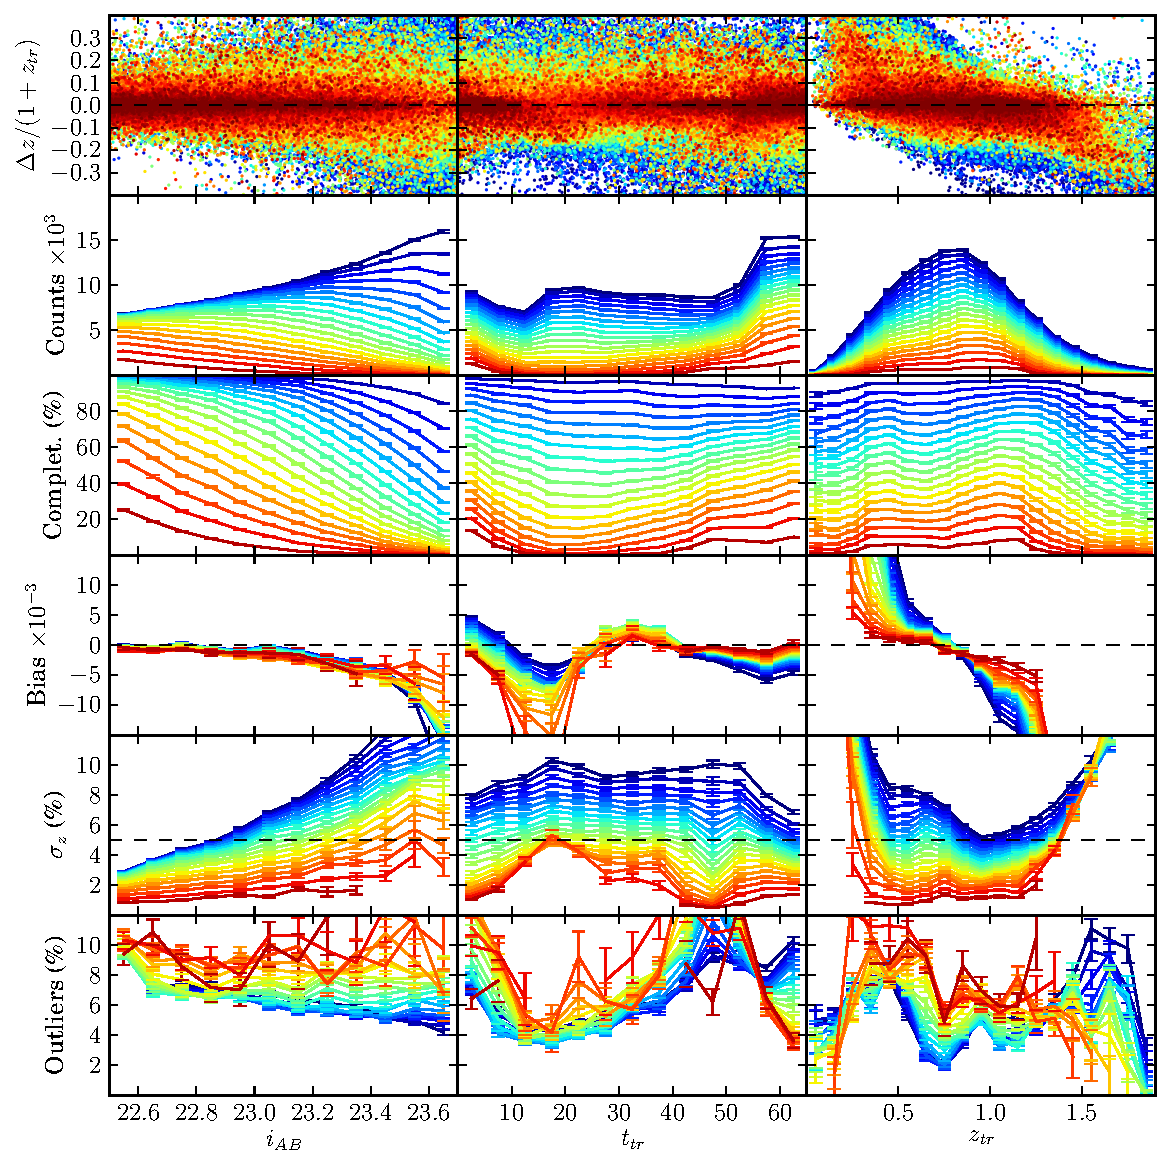
\includegraphics[type=pdf,ext=.pdf,read=.pdf, width=130mm]{./plots/mock.r260.n1e6.s10.121027_default_faint}
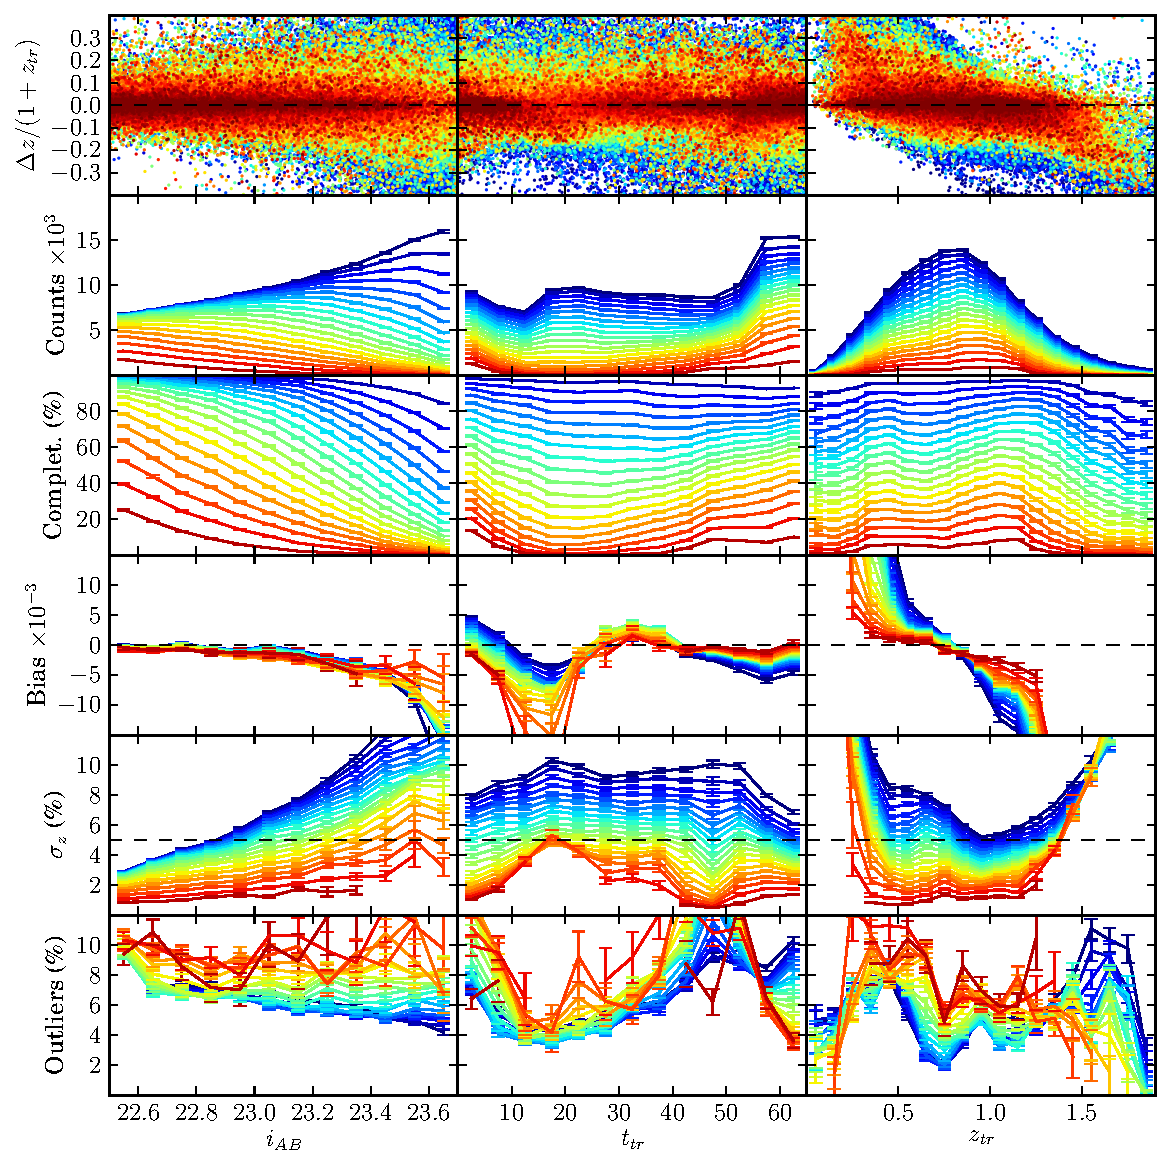
\includegraphics[type=jpg,ext=.jpg,read=.jpg, width=130mm]{./plots/mock.r260.n1e6.s10.121027_default_faint}
\caption{Statistics showing the PAU-FS photo-$z$ performance in the same layout as in Fig.~\ref{bs_pz_results}.}
\label{fs_pz_results}
\end{figure*}

\subsection{Narrow bands vs. Broad bands}
We want to quantify the improvement that the NB bring to the photo-$z$ performance. For this purpose, we run \texttt{BPZ} on the BS and the FS using the NB and the BB separately. Then, in Fig.~\ref{Dz_pau_only_BB} and Table~\ref{tab:usefulness_NB}, we compare the results between these runs and also with the original ones when the BB and the NB are used together (BB+NB). Figure~\ref{Dz_pau_only_BB} shows normalized $\Delta z/(1+z_{tr})$ distributions for the BS (red) and the FS (blue) using only the BB (dashed), only the NB (dotted) and both together BB+NB (solid). We see that the resulting distributions when using only BB (dashed) show overall shapes close to Gaussian with perhaps larger tails on both sides. However, when the NB are also included (solid) the peaks of the distributions become clearly sharper. This is more noticeable in the BS than in the FS, because the non-observed condition ($\sigma_m<0.5$) defined in Section~\ref{sec:mock} implies that most of the NB are not used in the photo-$z$ determination for the FS. Table~\ref{tab:usefulness_NB} shows bias (median), $\sigma_z$ ($\sigma_{68}$) and $3\sigma$-outlier fraction of each distribution. $\sigma_z$ in the BS is reduced $\sim$4.8 times going from $\sim$3.34\% to $\sim$0.7\% when the NB are included, while the improvement is much less significant in the FS. We also see that bias is reduced by an order of magnitude when the NB are included in both samples. On the contrary, the outlier fraction increases, but as mentioned, this is due to the fact that improvements on $\sigma_z$ penalize the outlier fraction. On the other hand, we see that using NB alone slightly degrades all metrics in the BS and the FS, except the outlier fraction in the FS which is improved for the same reason. In fact, $\sigma_z$ in the FS gets almost twice worse than when only using BB or BB+NB. It seems that in the FS NB by themselves only help the bias, while if they are used together with the BB, the improvement also extends to $\sigma_z$.
\begin{figure}
\centering
\includegraphics[height=84mm]{./plots/Dz_pau_only_BB.pdf}
\caption{Normalized $\Delta z/(1+z_{tr})$ distributions for the BS (red) and the FS (blue) using only BB (dashed), only NB (dotted) or both together BB+NB (solid). Bias, $\sigma_z$ and 3$\sigma$-outlier fraction of each distribution are shown in Table~\ref{tab:usefulness_NB}.}
\label{Dz_pau_only_BB}
\end{figure}

\begin{table}
\centering
\begin{tabular}{cccccccc}
\cline{2-4}
 & \multicolumn{3}{c}{Bright Sample} \\
\cline{2-4}
 & BB & NB & BB + NB \\
\cline{1-4}
\multicolumn{1}{c}{Bias$\times10^{-4}$} & -31.64 & -3.31 & -2.18 \\
\multicolumn{1}{c}{$\sigma_z$(\%)} & 3.34 & 0.83 & 0.70 \\
\multicolumn{1}{c}{Outliers(\%)} & 4.41 & 18.19 & 13.28 \\
\cline{1-4}
 & \multicolumn{3}{c}{Faint Sample} \\
\cline{2-4}
 & BB & NB & BB + NB \\
\cline{1-4}
\multicolumn{1}{c}{Bias$\times10^{-4}$} & -152.66 & -41.19 & -19.01 \\
\multicolumn{1}{c}{$\sigma_z$(\%)} & 9.38 & 16.17 & 8.86 \\
\multicolumn{1}{c}{Outliers(\%)} & 6.79 & 4.90 & 7.18 \\
\cline{1-4}
\end{tabular}
\caption{Bias (median), $\sigma_z$ ($\sigma_{68}$) and $3\sigma$-outlier fraction when using only BB, only NB or both together BB+NB for the bright and faint samples.}
\label{tab:usefulness_NB}
\end{table}


\subsection{Impact of the photo-$z$s on clustering}
We want to study the impact of the PAU photo-$z$ performance on the measurements of angular clustering. In \citet{Gaztanaga2012} it is shown that galaxy cross-correlation measurements $\bar{\omega}_{ij}$ between two photo-$z$ bins $i$ and $j$ are related to their cross-correlation between real redshift bins $\omega_{ij}$ as
\begin{equation}
\bar{\omega}^{A\times B}_{ij} = \sum_{kl} r^A_{ik} \omega^{A \times B}_{kl} r^B_{jl} = r_A \cdot \omega^{A \times B} \cdot  r^T_B,
\label{eq:wijbar}
\end{equation}
where $r_{ij}$ is called the migration matrix and gives the probability that a galaxy observed at the photo-$z$ bin $i$ will be actually at the true redshift bin $j$, while $A$ and $B$ denote different galaxy samples. We compute the migration matrices from the PAU photo-$z$ simulations and show them on Fig.~\ref{plot:rij} for the BS (top) and the FS (bottom) in photo-$z$ bins of width $0.014(1+z)$, which is four times the photo-$z$ precision $\sigma_z$ in the BS once the photo-$z$ quality cut that leaves a 50\% completeness is applied. Note that the matrices are normalized row-wise by definition. The FS migration matrix has quite a  thick diagonal, i.e. around $z_{tr} \simeq 1$ the width is $\Delta z \simeq 0.1$ for $\simeq 10\%$ probabilities and $\Delta z \simeq 0.4$ for $\simeq 1\%$. There are also outliers going from very large true redshifts 
$z_{tr} \simeq 1.8$ to lower photo-$z$ redshifts and some from low true redshifts up to  $z_{ph} \simeq 1$. The  BS has a 
thinner diagonal with $\Delta z < 0.04$ at $\simeq 1\%$ probability and with fewer outliers.
These values are of course in agreement with previous results in Figs.~\ref{dz_hist} and \ref{pz_results}.

\begin{figure}
\centering
\includegraphics[width=84mm]{./plots/rij_pau.pdf}
\caption{The resulting migration matrices $r_{ij}$ from the PAU photo-$z$ simulations after applying the photo-$z$ quality cut that leaves 50\% completeness. The top plot corresponds to the BS and the bottom plot to the FS. For a higher contrast and clarity we plot the logarithm of the matrix values. These matrices give the probability that a galaxy observed at the photo-$z$ bin $i$, will be actually at the true redshift bin $j$. The bin widths are $0.014(1+z)$, four times the photo-$z$ precision expected in the BS.}
\label{plot:rij}
\end{figure}

\begin{figure*}
\centering
\makebox[0cm]{\includegraphics[width=170mm]{./plots/wij_pau.pdf}}
\caption{Top panels show the angular auto (diagonal) and cross- (off-diagonal) correlations $\omega_{ij}$ at 1~arcmin between the true redshift bins $i$ and $j$ of the BS (left), the FS (middle) and the crossing of both of them (right). Bottom plots show the same correlations but measured with photo-$z$ bins, which can be computed by using Eq. (\ref{eq:wijbar}) with the migration matrices in Fig.~\ref{plot:rij}. The bin widths are $0.014(1+z)$, four times the photo-$z$ precision expected in the Bright Sample.}
\label{plot:wij}
\end{figure*}

To illustrate how these matrices affect angular clustering measurements, we use a simple model to
predict $\omega_{ij}$ at an arbitrary reference angular scale, $\theta$, of 1~arcmin. We include intrinsic
galaxy clustering and weak lensing magnification:
\begin{eqnarray}
\label{eq:all4}
w_{ij} &=& w_{G_iG_j}+ w_{G_i\mu_j} + w_{\mu_i  G_j}+ w_{\mu_i\mu_j} \\
w_{G_iG_j} &=&  b_ib_j \int dz_1dz_2  \, \, \phi_{G_i}(z_1) \, \phi_{G_j}(z_2)  \, \, \xi(r_{12}) \\
 w_{G_i\mu_j} & =&   b_i \alpha_j \int dz_1 dz_2 \, \,\phi_{G_i}(z_1) \, p_{\mu_j}(z_2) \, \, \xi(r_{12}) \\
w_{\mu_i\mu_j} & =&   \alpha_i \alpha_j \int dz_1 dz_2 \,  \, p_{\mu_i}(z_1) \, p_{\mu_j}(z_2) \, \, \xi(r_{12}) 
\end{eqnarray}
where $\xi(r_{12})$ is the non-linear matter 2-point correlation 
between the positions of two galaxies separated in 3D space by $r_{12}=r_2-r_1$, 
where the angular separation between $r_1$ and $r_2$ is fixed to be the reference angle (i.e. $\theta=1$ arcmin),
while the radial separation is integrated out via $z_1$ and $z_2$. We have that
$\phi_{G_i}(z)$ is a top-hat distribution for galaxies in the  redshift bin $i$  and $p_{\mu_j}(z)$ is the efficiency of weak
lensing effect for lenses at $z$ and sources at $z_j$ (following the notation in \citet{Gaztanaga2012}). 
The coefficient $b_i$ is the effective galaxy bias at $z_i$  and 
 $\alpha_j\equiv 2.5s_j-1$ is the amplitude of the weak lensing magnification effect (with $s_j$ the slope
of the galaxy number counts at the flux limit of the sample at $z_j$). 
The first equation above has 4 terms corresponding to galaxy-galaxy
(intrinsic clustering), galaxy-magnification, magnification-galaxy  and 
magnification-magnification correlations. In our test, we use $\alpha_i=1$ and $b_i=1$
to generate the starting point for $\omega_{ij}$. We then apply
the following transformation:
\begin{eqnarray}
\omega^{B\times B}_{ij} \rightarrow b_{B}(z_i)b_{B}(z_j)\omega_{ij} \\
\omega^{F\times F}_{ij} \rightarrow b_{F}(z_i)b_{F}(z_j)\omega_{ij} \\
\omega^{B\times F}_{ij} \rightarrow b_{B}(z_i)b_{F}(z_j)\omega_{ij}
\end{eqnarray}
depending on which galaxy samples we are cross-correlating (FS or BS), where
\begin{eqnarray}
b_{B}(z_i) &=& 2 + 2 (z_i - 0.5) \\
b_{F}(z_i) &=& 1.2 + 0.4 (z_i - 0.5)
\end{eqnarray}
are the biases in the BS and FS respectively in the photo-$z$ bin $i$ (at mean redshift $z_i$). This corresponds
to using linear bias for the intrinsic  correlation (as in \citet{Gaztanaga2012}) and some particular evolving
slope ($s_i \sim 1$) for the magnification cross-correlations.
 In Fig.~\ref{plot:wij} we show $\omega^{B\times B}_{ij}$ (left), $\omega^{F\times F}_{ij}$ (middle) and $\omega^{B\times F}_{ij}$ (right) before (top) and after (bottom) being transformed by the migration matrices $r_{ij}$ in Fig.~\ref{plot:rij} through Eq. (\ref{eq:wijbar}). Note that for the $B\times B$ and $F \times F$ cases the correlations matrices are symmetrical. Also note that the redshift ranges in both samples are different, so that the $B \times F$ correlation matrix is not squared.

 In the top panels, we can see the
intrinsic galaxy-galaxy clustering in the diagonal of the matrix, which has an amplitude of order unity and
decreases rapidly to zero for separated redshift bins. 
The galaxy-magnification correlation appears as a diffused off-diagonal cloud with an 
amplitude $<0.05$ (clear colors). The magnification-magnification contribution is negligible.
In the bottom panel, we see the effect of the photo-$z$ migration. The diagonal
(auto-correlations) becomes thicker and diluted. The off-diagonal galaxy-magnification cloud becomes
 more diffused, especially for the FS. The cross-correlation $F \times B$ produces results that are intermediate
between $B \times B$ and $F \times F$.

We can invert the migration matrices to go from the bottom
panels (which are the observations $\bar{\omega}^{A\times B}$) to the top panels (i.e. true correlations
$\omega^{A \times B}$) by inverting Eq. (\ref{eq:wijbar}):

\begin{equation}
 \omega^{A \times B} = r_A^{-1} \cdot \bar{\omega}^{A\times B}  \cdot  (r^T_B)^{-1} 
\label{eq:wij}
\end{equation}
This should work perfectly well if we can calibrate the $r_{ij}$ matrices properly. For a large
fiducial survey with about 5000 sq. deg. we need about $\simeq 1\%$ accuracy in $r_{ij}$
\citep{Gaztanaga2012}. In practice, the accuracy of the above reconstruction
 can be used to put requirements on the photo-$z$ calibration.

\section{Optimization of the PAU filter set}
\label{sec:opti}

In this section we want to explore how the photo-$z$ performance changes under variations of the PAU NB filter set. 

\subsection{NB filter set variations}
We study five variations of the original NB filter set whose response is shown in Fig.~\ref{pau_filt_sets}. All the variations conserve the number of filters. In the order that appear in Fig.~\ref{pau_filt_sets}, the proposed filter sets are:

\begin{table}
\centering
\caption{Global photo-$z$ performance results for each filter set shown in Fig.~\ref{pau_filt_sets}.  Photo-$z$ performance is characterized through the three metrics: bias (median), $\sigma_z$ ($\sigma_{68}$) and the $3\sigma$-outlier fraction. Photo-$z$ quality cuts resulting in a 50\% \ overall completeness are applied in all cases. We show results for the
Bright Sample (BS) and Faint Sample (FS).}
\begin{tabular}{lccc}
 & Bias & $\sigma_z$(\%) & Outliers(\%) \\
\hline
Default BS & -0.71$\cdot10^{-4}$ & 0.34 & 3.02
\\
Default FS & -1.33$\cdot10^{-3}$ & 4.73 & 7.36
\\
\hline
Blueshift BS &-2.11$\cdot10^{-4}$ & 0.38 &  3.23
\\
Blueshift FS & -3.11$\cdot10^{-3}$ & 5.19 & 7.05
\\
\hline
Redshift BS &-0.74$\cdot10^{-4}$  & 0.35 &   3.31
\\
Redshift FS &  -0.65$\cdot10^{-3}$  & 4.99 & 7.21
\\
\hline
Log BS &-0.69$\cdot10^{-4}$  & 0.35 &   2.80
\\
Log FS &  -1.46$\cdot10^{-3}$  & 4.73 & 7.43
\\
\hline
x1.5 width BS &-3.18$\cdot10^{-4}$  & 0.45 &   3.00
\\
x1.5 width FS &  -2.76$\cdot10^{-3}$  & 3.87 & 7.76
\\
\hline
x0.5 width BS &-0.00$\cdot10^{-4}$  & 0.32 &   5.22
\\
x0.5 width FS &  -0.99$\cdot10^{-3}$  & 6.91 & 5.52
\\
\hline
\end{tabular}
\label{tab:pz_results_filt_sets}
\end{table}

\begin{figure*}
\centering
\includegraphics[height=130mm]{./plots/pau_filt_sets.pdf}
\caption{On the top-left, the original PAU NB filter set (same as in Fig.~\ref{pau_effective_bands}). The rest are the five variations to be compared in terms of photo-$z$ performance. Grayed areas show the covered wavelength range by the \texttt{Default} filter set. In descending order from left to right we have: the \texttt{Log} filter set with the same overall range as the \texttt{Default} but with band widths that increase logarithmically; the \texttt{Blueshift} filter set, which is the same as the \texttt{Default} but with the bands shifted 1000\AA \ towards bluer wavelengths; the \texttt{Redshift} filter set which is the same as \texttt{Default} but shifted towards redder wavelengths; the \texttt{$\times$0.5 width} filter set whose band widths are half those of the \texttt{Default} ones; and the \texttt{$\times$1.5 width} filter set whose bands are 1.5 times wider. The overall wavelength ranges of these last two set-ups are chosen to be centered with respect to the range of the \texttt{Default} set.}
\label{pau_filt_sets}
\end{figure*}

\begin{itemize}
\item \textbf{Default:} This is the default filter set already shown in Fig.~\ref{pau_effective_bands}. 
\item \textbf{Log:} In this filter set, band widths increase in wavelength logarithmically, so that they fulfill $\lambda_0 / \Delta \lambda=const.$, where $\Delta \lambda$ is the width of the rectangular part of the band (without taking into account the lateral wings) and $\lambda_0$ is the central wavelength of the band. We impose the overall wavelength range covered by the set of bands to be the same as for the \texttt{Default} filter set. Given that the total number of bands is kept at 40, we obtain that the bluest filter has a width of 97\AA, while the reddest is 159\AA \ wide. The reason for this filter set is that, when spectra are redshifted, their spectral features are moved to redder wavelengths, but also their widths are stretched as $\Delta \lambda ' = (1+z) \Delta \lambda$. If the photo-$z$ determination depends strongly on the tracking of any spectral feature, such as the 4000\AA \ break in elliptical galaxies, a filter set like \texttt{Log} will continue to enclose the same fraction of the spectral feature in a single filter independently of how redshifted is the spectrum.
\item \textbf{Blueshift:} This is the same as the \texttt{Default} filter set, however bands have been shifted 1000\AA \ towards bluer wavelengths. We expect to get better photo-$z$ performance at low redshift and for late-type galaxies. The down side of this filter set is that the overall response turns out to be very inefficient in the ultraviolet zone (middle-left of Fig.~\ref{pau_filt_sets}), like it was for the \textit{u} band.
\item \textbf{Redshift:} This is the same variation as before but shifting bands 1000\AA \ towards redder wavelengths. We expect to get better photo-$z$ performance at high redshift and for early-type galaxies. This filter set does not suffer from the problem of the ultraviolet, so its band responses are much more uniform over the covered range (middle-right of Fig.~\ref{pau_filt_sets}). On the other hand, the sky brightness on this region is higher.
\item \textbf{$\times$0.5 width:} This is a filter set whose band widths are half of the \texttt{Default} ones. Lateral wings are also reduced to half of their size, from 25\AA \ to 12.5\AA, in order to avoid an excessive overlap between adjacent bands. We expect to improve the photo-$z$ precision, at least for galaxies with good Signal-to-Noise ratio on their photometry. The down side of this filter set is that, since the number of bands is kept, the overall wavelength range covered is also reduced by a half. We choose it to be centered with respect to the \texttt{Default}, so that it covers from 5500\AA \ to 7500\AA, roughly spanning only from the bluest filter of the \texttt{Redshift} set to the reddest of the \texttt{Blueshift} set. This can lead to a degradation of the photo-$z$s at very low and high redshift, although the broad bands may attenuate this effect.
\item \textbf{$\times$1.5 width:} This is a filter set whose band widths are 1.5 times wider than the \texttt{Default} ones. Because of this, we expect a significant degradation of the photo-$z$ precision for galaxies with good Signal-to-Noise ratio on their photometry. However, the increase in $S/N$ may help. Moreover, the covered wavelength range also increases by 50\%. We choose the new range to be centered with respect to the \texttt{Default} set, so that it covers from 3500\AA \ to 9500\AA, roughly from the bluest edge of the \texttt{Blueshift} set to the reddest edge of the \texttt{Redshift} set, so we expect to see a more uniform photo-$z$ performance over the whole redshift range.
\end{itemize}

We generate magnitudes for each filter set band as described in Section~\ref{sec:mock} using the same exposure times per NB filter tray and BB as in the \texttt{Default} filter set. We do not try to optimize the exposure times for each filter set. The aim of this study is to see how, in spite of this, the photo-$z$ performance changes. Once the new photometric mock catalogs are created, they are also split into a Bright Sample ($i_{AB}<22.5$) and Faint Sample ($22.5<i_{AB}<23.7$). We run BPZ on each catalog using the same settings as for the \texttt{Default} filter set. There is no need to calibrate a different prior for each filter set, since the prior was initially calibrated on the broad band $i$, which is shared by all these filter sets. Photo-$z$ quality cuts resulting in an overall completeness of $\sim$50\% are applied in all cases.
\begin{figure*}
\centering
\includegraphics[type=pdf,ext=.pdf,read=.pdf, width=130mm]{./plots/mock.r260.n1e6.s10.121027_bright_filt_sets_compar} \\
\includegraphics[type=pdf,ext=.pdf,read=.pdf, width=130mm]{./plots/mock.r260.n1e6.s10.121027_faint_filt_sets_compar}
\caption{Photo-$z$ performance metrics using the different filter sets shown in Fig.~\ref{pau_filt_sets}. Rows: Completeness after applying a photo-$z$ quality cut leading to a 50\% global completeness; bias (median); $\sigma_z$ ($\sigma_{68}$) and 3$\sigma$-outlier fraction, as a function of $i_{AB}$, $t_{tr}$ and $z_{tr}$ (columns), in the BS (top) and the FS (bottom).}
\label{pz_results_filt_sets}
\end{figure*}

\subsection{Global photo-$z$ performance}
Global photo-$z$ performance results for each filter set are shown on Table~\ref{tab:pz_results_filt_sets}, using the same metrics as in Section~\ref{sec:photoz}: bias (median), $\sigma_z$ ($\sigma_{68}$) and the $3\sigma$-outlier fraction. We find that the \texttt{$\times$0.5 width} set gives the best bias (it completely vanishes), and $\sigma_z$ ($\sim$6\% better than \texttt{Default}) in the BS, while in the FS it is the \texttt{Redshift} set which gives the best bias ($\sim$54\% better) and the \texttt{$\times$1.5 width} set which gives the best $\sigma_z$ ($\sim$18\% better). On the other hand, the \texttt{$\times$1.5 width} set gives the worst bias (a factor 4.6 worse) and $\sigma_z$ ($\sim$32\% worse) in the BS, while in the FS it is the \texttt{Blueshift} set which gives the worst bias (a factor 2.4 worse) and the \texttt{$\times$0.5 width} which gives the worst $\sigma_z$ ($\sim$46\% worse). Regarding the outlier fraction, its direct comparison is trickier since it depends on the value of $\sigma_z$. Even so, we see that in the BS the \texttt{Log} set gives the best value, while in the FS the \texttt{$\times$0.5 width} set gives the worst. 

The general conclusions are that the \texttt{Log} set gives almost the same photo-$z$ performance as the \texttt{Default} set, with a slight increase of $3\%$ in $\sigma_z$ in the BS. Therefore, we see that the logarithmic broadening of the band widths does not suppose any global improvement. On the other hand, and as we expected, if the Signal-to-Noise ratio in the photometry is good enough, the narrower the bands, the better the photo-$z$ performance results. On the other hand, wider bands are the ones that give better photo-$z$ precision in the FS, because there are more bands that pass the cut $\sigma_m<0.5$ introduced in Section~\ref{sec:mock}. 

\subsection{Results as a function of $i_{AB}$, $t_{tr}$ and $z_{tr}$}
In Fig.~\ref{pz_results_filt_sets} we show plots similar to those in Figs.~\ref{bs_pz_results} and \ref{fs_pz_results} with the photo-$z$ performance metrics as a function of $i_{AB}$, $t_{tr}$ and $z_{tr}$ for the BS (top) and the FS (bottom) when using the different filter sets of Fig.~\ref{pau_filt_sets}. Black curves correspond to the photo-$z$ results of the \texttt{Default} filter set when the 50\% completeness photo-$z$ quality cut is applied, and we will treat them as the reference results. The rest of curves in different colors correspond to the variations of the \texttt{Default} filter set. As a general trend, we see that these curves do not deviate much from the reference. Even so, we will discuss each case separately. 

In the BS, we see that redshifting the bands (red curves) slightly degrades the completeness at low magnitudes up to $i_{AB}<21.5$. As was expected, all the metrics also degrade at low $z_{tr}$. In contrast, blueshifting the bands (blue curves) shows the opposite behavior, a degradation of all the metrics at high $z_{tr}$. This is due to the lack of coverage at blue and red wavelengths respectively of each filter set, as we have already mentioned before. Something similar happens for the \texttt{$\times$0.5 width} set, where band widths, and consequently the covered wavelength range, is reduced by a half (green curve). The resulting photo-$z$ performance is worse at both low and high $z_{tr}$. However, the photo-$z$ precision $\sigma_z$ is slightly better at intermediate redshifts ($0.15<z_{tr}<0.5$), for spiral galaxies ($10<t_{tr}<30$) and at bright magnitudes ($i_{AB}<20.5$). Increasing the band width by a factor 1.5 (cyan curve) does not result in an improvement in any case. Bias and $\sigma_z$ degrade all over the range of the three variables, $i_{AB}$, $t_{tr}$ and $z_{tr}$. This is in full agreement with the results shown in Table~\ref{tab:pz_results_filt_sets}, where this filter set was seen as giving the worst photo-$z$ performance. Also in agreement with Table~\ref{tab:pz_results_filt_sets}, we see that the \texttt{Log} filter set practically does not introduce any change from the \texttt{Default} filter set. 

In the FS we do not observe big differences between the completeness curves, but for example the \texttt{Blueshift} filter set shows slightly lower completeness for elliptical galaxies than for irregulars, unlike the \texttt{Redshift} and \texttt{$\times$0.5 width} filter sets, which show the opposite behavior. In the $z_{tr}$ range we also recognize similar behaviors as in the BS, as for example the fact that the \texttt{Blueshift} filter set shows better completeness at low $z_{tr}$ and worse at high, as well as the opposite behavior of the \texttt{Redshift} and \texttt{$\times$0.5 width} filter sets. The \texttt{Blueshift} filter set seems to cause a significant degradation in the bias for faint, spiral and high redshift galaxies, and also delivers a considerably worse $\sigma_z$ than the \texttt{Default} over all the ranges. In return, the \texttt{Redshift} filter set shows better bias at high magnitudes and redshifts. On the other hand, we observe that the \texttt{$\times$0.5 width} filter set shows much more pronounced trends on the bias, in particular at $i_{AB}>23.1$, spiral galaxies and over all the $z_{tr}$ range, where values are substantially worse than for the \texttt{Default} filter set. As in Table~\ref{tab:pz_results_filt_sets}, we observe that the worst $\sigma_z$ is found for the \texttt{$\times$0.5 width} filter set, while the best is for the \texttt{$\times$1.5 width} filter set over all the ranges. This is exactly the opposite to the behavior seen for the BS. 
In general, narrower bands are useful in the BS, but not in the FS.  

\section{Discussion and Conclusions}
\label{sec:discussion}
In the previous sections, we have seen that, at the level of simulated data, a photo-$z$ precision of $\sigma_z \sim 0.0035(1+z)$ can be achieved for $\sim$50\% of galaxies at $i_{AB}<22.5$ by using a photometric filter system of 40 narrow bands of 125\AA \ width together with the \textit{ugrizY} broad bands. The precision degrades to $\sigma_z \sim 0.05(1+z)$ when we move to the magnitude range $22.5<i_{AB}<23.7$. These coincide with the two photo-$z$ precision requirements defined in \citet{Gaztanaga2012} needed to simultaneously measure Redshift Space Distortions (RSD) and Magnifications bias (MAG) on two samples, one on the foreground and one on the background, over the same area of the sky. The galaxies removed are the ones with the worst photo-$z$ quality according to our photo-$z$ algorithm used. In \paperodds\ it is shown that this kind of cuts, when they remove a substantial fraction of galaxies, can grossly bias the measured galaxy clustering. However, in the same \doctype\ \we\ propose a way to correct for it. 

On the other hand, we found that spiral galaxies are the ones that give the worst photo-$z$ performance. Moreover, quality cuts mostly remove them. Contrary to what was assumed in \cite{Benitez2009}, elliptical galaxies do not provide the best photo-$z$ performance, but irregular galaxies with prominent emission lines at $\sim$3737\AA \ [OII] and $\sim$5000\AA \ [OIII] are actually the ones that give the best performance. A possibility is that these two emission lines are better traced by the narrow bands than a single feature as the 4000\AA \ break of elliptical galaxies, making the photo-$z$ determination more robust. 

We also studied the effect of including the 40 narrow bands in a typical broad band filter set \textit{ugrizY}. We find that the $\Delta z / (1+z_{tr})$ distributions become more peaky around the maximum moving away from Gaussianity. Bias improves by an order of magnitude. Precision also improves in a factor of $\sim$5 below $i_{AB}\sim22.5$. However, the low signal-to-noise in narrow bands makes the improvement very small within $22.5<i_{AB}<23.7$, concluding that narrow bands at faint magnitudes are useful to improve the bias but not the precision.

We have also estimated the photo-$z$ migration matrices $r_{ij}$ which correspond to the probability
 that a galaxy observed at the photo-$z$ bin $i$ is actually at the true redshift bin $j$.
These are shown  in Fig.~\ref{plot:rij} for both the BS and FS.  We then show (in Fig.~\ref{plot:wij})
how this photo-$z$ migration matrix $r$ distorts the observed auto and cross-correlation of galaxies in narrow redshift bins.
 We show results for both the intrinsic clustering, which dominates the diagonal in the measured angular 
cross-correlation matrix,  $\bar{\omega}$, and the magnification effect, which appears as a diffused
off-diagonal cloud in $\bar{\omega}_{ij}$. The true cross-correlation matrix $\omega_{ij}$ 
can be obtained from the inverse migration $r^{-1}$  with a simple matrix operation: 
$\omega = r^{-1}\cdot\bar{\omega}\cdot(r^T)^{-1}$. This is a standard deconvolution problem, and it is only limited
by how well we know the migration matrix.

We find that introducing slight variations on the 40 narrow band filter set, such as: shifting bands to higher/lower wavelengths, narrowing/broadening or increasing logarithmically band widths, do not introduce significant changes on the final photo-$z$ performance.  Even so, general trends are that narrowing/broadening bands improves/worsens the photo-$z$ performance below/above $i_{AB}\sim22.5$, while red/blueshifting bands improve the photo-$z$ performance at high/low redshifts and the quality-cuts efficiency for early/late-type galaxies. Logarithmically growing band widths do not turn into any measurable improvement. Therefore, we conclude that the initial proposed filter set of 40 narrow bands seems to be close to optimal for the purposes of the PAU Survey at the WHT.

Additionally, we have also tried doubling the exposure times in all bands. The magnitude limits become $\sim0.5$~mag deeper, so that the new bright sample goes down to $i_{AB}<23$ and the new faint sample down to $i_{AB}<24.1$. Within these magnitude limits, the photo-$z$ performance remains almost unchanged, and we still reach the requirement in $\sigma_{68}$ after removing $\sim50$\% of the galaxies in both the new bright and the new faint catalogs. On the other hand, if we stick to the initial magnitude limits while still doubling the exposure times, we find that in this case the requirements are reached by removing only 30\% of the galaxies in the bright sample and none in the faint.


\chapter{Photo-$z$ quality cuts and their impact on the measured galaxy clustering}
\chaptermark{Photo-$z$ quality cuts and their impact on galaxy clustering}
\label{ch:odds}
\ExecuteMetaData[./odds_paper/introduction.tex]{tag1}

\ExecuteMetaData[./odds_paper/introduction.tex]{tag2}

\ExecuteMetaData[./odds_paper/introduction.tex]{tag3}
\section{Data Samples}
\label{sec:data}

The Mega-Z LRG DR7\footnote{An ASCII version of the Mega-Z LRG DR7 catalog can be found at \url{http://zuserver2.star.ucl.ac.uk/~sat/Mega-Z/Mega-ZDR7.tar.gz.}} catalog \citep{Collister2007} includes $\sim$1.4 million Luminous Red Galaxies from the SDSS Data Release 7 in the redshift range $0.4< z < 0.7$, with limiting magnitude $i_{AB}<20$. It covers an area of $\sim$7750~deg$^2$ of the sky that is displayed in Fig.~\ref{scatter_map}. This is the sample in which we will investigate the effect of the photo-z quality cuts on the observed galaxy clustering. 

\begin{figure*}
\centering
\includegraphics[type=pdf,ext=.pdf,read=.pdf, width=130mm]{./plots/scatter_map}
\caption{Mega-Z and 2SLAQ maps in Mollweide projection plotted in blue and red respectively. For the sake of clarity only a hundred thousand galaxies randomly selected from Mega-Z and five thousand from 2SLAQ have been plotted. The Mega-Z sample covers a total of 7750~deg$^2$, while 2SLAQ covers 180~deg$^2$. The 2SLAQ area is divided into several fields inside a 2$^\circ$-wide strip that extends along the celestial equator.} 
\label{scatter_map}
\end{figure*}

In order to calibrate the photometric redshifts of the Mega-Z galaxies, a representative galaxy sample with known redshifts is needed.  Fortunately, such a sample exists: the 2dF-SDSS LRG and Quasar\footnote{The whole 2SLAQ data can be downloaded from \url{http://www.2slaq.info/query/2slaq_LRG_webcat_hdr.txt.}} (2SLAQ) catalog \citep{Cannon2006} was obtained using the same selection criteria as the Mega-Z catalog and includes $\sim$13100 LRGs with spectroscopic redshifts. Its sky coverage of only 180~deg$^2$ can be seen in Fig.~\ref{scatter_map} in red. The galaxies are located on a strip of 2~deg along the celestial equator, the area subtended by the 2dF spectrograph. Only non-repeated objects ($ind=1$) with high spectroscopic redshift confidence level ($hqs\ge3$) are used in this analysis. 

The selection criteria in both catalogs consist of a magnitude cut and several color cuts. All magnitudes have been corrected for galactic extinction;  we use model magnitudes for the color cuts and to compute the photometric redshifts (section~\ref{sec:photoz}). The magnitude cut 
\begin{equation}
17.5<i_{deV}<19.8
\label{mag_cut}
\end{equation}
is motivated by the limiting magnitude of the 2dF spectrograph and to ensure completeness of the 2SLAQ catalog. While the Mega-Z catalog is complete up to magnitude $i_{deV}=20$, the 2SLAQ completeness drops off sharply beyond $i_{deV}=19.8$, so the cut forces us to cut the Mega-Z sample at this limit. It eliminates $\sim$32\% of the Mega-Z galaxies leaving a total of $\sim$950000. The $i_{deV}$ magnitude distribution for both samples is plotted on the bottom-right of Fig.~\ref{Nm_megaz}. The purple lines represent the cut in~(\ref{mag_cut}).

\begin{figure*}
\centering
\includegraphics[type=pdf,ext=.pdf,read=.pdf, width=150mm]{./plots/Nm_megaz}
\caption{From top-left to bottom-right, the model magnitude distributions in the $ugriz$ bands for 2SLAQ in red and Mega-Z in black, normalized to each other. The last plot corresponds to the $i$ band de Vaucouleurs magnitude. All magnitudes are corrected for galactic extinction. The purple lines in the last plot show the magnitude cut 
in~(\ref{mag_cut}), which is the nominal limiting magnitude for the 2SLAQ sample. The agreement is excellent, except in the $u$ band, where the low signal-to-noise produces a small disagreement around magnitude $\sim$25.}
\label{Nm_megaz}
\end{figure*}

The color cuts applied are: 
\begin{eqnarray}
0.5<g-r&<&3 \label{gr_isol_lrg}\\
r-i&<&2 \label{ri_isol_lrg}\\
c_\parallel \equiv 0.7(g-r)+1.2(r-i-0.18)&>&1.6 \label{later_type}\\
d_\perp \equiv (r-i)-(g-r)/8.0&>&0.55 \label{zp_cut} \, .
\end{eqnarray}
They are used to isolate the LRGs from the rest of galaxies. In particular, (\ref{later_type}) separates later-type galaxies from LRGs, and (\ref{zp_cut}) acts as an implicit photo-z cut of $z\gtrsim0.45$, as we will see in the next section.
In~\citet{Collister2007} the $d_\perp$ cut is set to 0.5 for the Mega-Z catalog, but, once again, the 2SLAQ completeness within $0.5<d_\perp<0.55$ is very poor: once all other cuts are applied, they represent 3.6\% of the galaxies, instead of 27\% in Mega-Z. Therefore, we choose $d_\perp > 0.55$.

These magnitude and color cuts leave a total of 749152 objects in the Mega-Z catalog and 11810 in the 2SLAQ catalog. In Figs.~\ref{Nm_megaz} and \ref{colors_megaz}, we plot the model magnitude distributions and the color-color scatters, respectively, for all the $ugriz$ bands, after applying all cuts. 2SLAQ is shown in red and Mega-Z in black. Solid and dashed lines represent the cuts. The 2SLAQ magnitude distributions have been normalized up to the total amount of galaxies in Mega-Z. The agreement between both catalogs is excellent, so that we can conclude that 2SLAQ is a representative spectroscopic sample of Mega-Z.
\begin{figure*}
\centering
\includegraphics[type=pdf,ext=.pdf,read=.pdf, width=130mm]{./plots/colors_megaz}
\caption{Color-color diagrams for both the Mega-Z catalog in black and the 2SLAQ catalog in red. For the sake of clarity, we have only plot a hundred-thousand galaxies for Mega-Z and five thousand for 2SLAQ. We can see that 2SLAQ covers the same color area as Mega-Z, so that we can conclude that it is a good representative spectroscopic sample. The blue and green dashed lines show the color cuts in (\ref{gr_isol_lrg}) and (\ref{ri_isol_lrg}) respectively, while the purple solid lines show the cuts in (\ref{later_type}) and (\ref{zp_cut}), used to select LRGs and high-z galaxies, respectively. The two last cuts shown in the top-right plot translate into an implicit cut of $r-i>0.72$ in the bottom plot.}
\label{colors_megaz}
\end{figure*}

Additionally, some extra cuts have been applied in the Mega-Z catalog to reduce the star contamination:
\begin{eqnarray}
i_{psf}-i_{model}&>&0.2\times(21.0-i_{deV})\\
i\text{-band de Vaucouleurs radius}&>&0.2\\
\delta_{sg} &>& 0.2
\end{eqnarray}
As explained in~\citet{Collister2007}, the first two cuts separate galaxies from stars leaving a residual $\sim$5\% contamination of M-type stars, which cannot be trivially separated either using $gri$ colors or through cuts on the subtended angular diameter. Because of this, the last cut is applied. First, the photo-z neural network ANNz~\citep{Collister2004} is trained on the 2SLAQ catalog that contains reliable information about whether objects are stars or galaxies. The trained network is then run on the whole Mega-Z catalog to compute the probability $\delta_{sg}$ that objects be galaxies. Removing all objects with probability below 0.2 reduces the stellar contamination from 5\% to 2\%~\citep{Collister2007}. In 2SLAQ, we can remove stars by simply getting rid of all those objects with redshift less than 0.01. 

\section{Photometric redshifts}
\label{sec:photoz}

We will perform the galaxy clustering study in several photometric redshift (photo-z) bins. Therefore, we will need to estimate the photo-z of each galaxy in the Mega-Z sample. Furthermore, the theoretical predictions for the clustering need the true-redshift distribution of the galaxies in each photo-z bin $i$, $N_i(z)$, which we can obtain from the 2SLAQ sample. 
For this purpose, we need to compute photometric redshifts of the 2SLAQ galaxies, split them into several photo-z bins, and, finally, recover the spectroscopic redshift distribution in each bin. Additionally, we will study the photo-z performance using 2SLAQ, and apply photo-z quality cuts to improve it. The impact of these cuts on $N_i(z)$ will also be studied.

We use the Bayesian Photometric Redshifts\footnote{\texttt{BPZ} can be found at \url{http://www.its.caltech.edu/~coe/BPZ/}.} (BPZ) template-fitting code described in~\citet{Benitez2000} to compute the photometric redshift of galaxies in both catalogs. It uses Bayesian statistics to produce a posterior probability density function $p(z|m_i)$ that a galaxy is at redshift $z$ when its magnitudes are $m_i$:
\begin{equation}
p(z|m_i) \propto \sum_t L(m_i|z,t) \, \Pi(z,t \mid m_i)  \, ,
\label{pz}
\end{equation} 
where $L(m_i|z,t)$ is the likelihood that the galaxy has magnitudes $m_i$, if its redshift is $z$ and its spectral type $t$, and $\Pi(z,t \mid m_i)$ is the prior probability that the galaxy has redshift $z$ and spectral type $t$. Finally, the photometric redshift $z(phot)$ of the galaxy will be taken as the position of the maximum of $p(z|m_i)$.

Each spectral type $t$ can be represented by a galaxy template. BPZ includes its own template library, but we prefer to use the new \texttt{CWW} library from \texttt{LePhare}\footnote{The new \texttt{CWW} library can be found in the folder \tt{/lephare\_dev/sed/GAL/CE\_NEW/} of the \texttt{LePhare} package at \url{http://www.cfht.hawaii.edu/~arnouts/LEPHARE/DOWNLOAD/lephare\_dev\_v2.2.tar.gz}.}, another template-based photo-z code described in \citet{Arnouts1999,Ilbert2006}. Both libraries are based on \citet{Coleman1980,Kinney1996}, but \texttt{BPZ} contains only 8 templates compared to 66 in~\texttt{LePhare}. The large number of templates allows us to focus on the LRG templates, which correspond to the genuine galaxy type of our catalogs. In particular, we select four: \texttt{Ell\_01}, \texttt{Ell\_09}, \texttt{Ell\_19} and \texttt{Sbc\_06}, and then we create nine interpolated templates between consecutive templates, giving a total of 31 templates, shown in Fig.~\ref{2slaq_templates}.

\begin{figure}
\centering
\includegraphics[type=pdf,ext=.pdf,read=.pdf, width=80mm]{./plots/2slaq_templates}
\caption{The spectral galaxy templates used in the determination of the 2SLAQ and Mega-Z photo-zs. There are a total of 31 templates that range from elliptical galaxies, the vast majority in both samples, to Sbc spiral galaxies.}
\label{2slaq_templates}
\end{figure}
Template-based photo-z codes require the knowledge of the filter band-passes of the survey instrument in order to compute the predicted photometry that will be compared with the observations to produce the likelihood $L(m_i|z,t)$. The SDSS instrument carries five broad-band filters, \textit{ugriz}, described in \citet{Fukugita1996}, whose throughputs are obtained from~\url{http://home.fnal.gov/~annis/astrophys/filters/filters.new}.

A crucial point of \texttt{BPZ} is the prior probability $\Pi(z, t \mid m)$ that helps improve the photo-z performance. \citet{Benitez2000} proposes the following empirical function:
\begin{equation}
\Pi(z, t \mid m) \propto f_t e^{-k_t(m-m_0)} \cdot z^{\alpha_t}\exp \left\lbrace -\left[ {z \over z_{mt}(m)} \right]^{\alpha_t} \right\rbrace,
\label{prior}
\end{equation}
where $z_{mt}(m) = z_{0t} + k_{mt}(m-m_0)$. Every spectral type $t$ has associated a set of five parameters $\lbrace f,k,\alpha,z_0,k_{m} \rbrace$ that determine the shape of the prior. These parameters are determined from the spectroscopic data themselves. In principle, we could assign one prior $\Pi(z, t \mid m)$ to each one of the 31 templates in Fig.~\ref{2slaq_templates}, but this would give a total of $31\times5=155$ parameters, too many for the spectroscopic data sample available. Instead, we split the 31 templates in two groups: $t=1$, with the 10 first templates that make up the group of pure elliptical galaxies, and $t=2$ with the rest. Then, running \texttt{BPZ} on 2SLAQ a first time, without priors, we find the group each galaxy belongs to. Fitting~(\ref{prior}) to this output, together with the spectroscopic redshifts and the observed magnitudes in one band (we choose the $i$ band), we find the values of the prior parameters. Results are given in Table~\ref{tab:prior}.
\begin{table}
\centering
\begin{tabular}{cccccc}
\hline
$t$ & $f$ & $k$ & $\alpha$ & $z_0$ & $k_{m}$ \\ \hline
1 & 0.72 & 0.0 & 8.679 & 0.477 & 0.078\\
2 & 0.14 & 0.0 & 7.155 & 0.488 & 0.064\\
\hline
\end{tabular}
\caption{The values of the prior parameters of (\ref{prior}) for the 2SLAQ galaxies.}
\label{tab:prior}
\end{table}

The $k$ parameters are related to the migration of galaxies from one spectral type to another at different magnitudes. The fit gives values of $k$ very close to 0, so we impose explicitly not having type migration by setting them exactly to 0. $f$ gives the fraction of galaxies of each type at magnitude $m_0$, which we choose to be $m_0=18.5$. Since $k=0$, we find that the 72\% of the galaxies belong to the spectral type group 1 independently of the magnitude, confirming that most of the galaxies are purely elliptical.

We define galaxies with catastrophic redshift determinations as those with $|\Delta z| \equiv |z(phot) - z(spec)| > 1$, where $z(spec)$ is the spectroscopic redshift and $z(phot)$ the photo-z. With the help of the prior, we are able to remove all these catastrophic redshift determinations, which account for $\sim$4.2\% of the 2SLAQ sample. They are typically galaxies with degeneracies in their color space, which cause confusions in the template fit and result in a photo-z much larger than the real redshift. Defining the photo-z precision $\sigma_z$ as half of the symmetric interval that encloses the 68\% of the $\Delta z$ distribution area around the maximum, we also find that its value for the non-catastrophic determinations improves by a factor 1.7, down to $\sigma_z \sim0.042$, in agreement with \citet{Padmanabhan2005,Collister2007,Thomas2011b}.

We also apply a cut on the quality of the photometry, consisting of not using any band, for each galaxy, with magnitude error $>$0.5. This cut mostly removes the information from the \textit{u} band for many galaxies, since the signal-to-noise tends to be lower in this band. The overall precision improves slightly to $\sigma_z \sim0.041$.

Photo-z codes, besides returning the best estimate for the redshift, typically also return an indicator of the photo-z quality. It can be simply an estimation of the error on $z(phot)$, or something more complex, but the aim is the same. In \texttt{BPZ}, this indicator is called \textit{odds}, and, it is defined as
\begin{equation}
odds = \int^{z(phot)+\delta z}_{z(phot)-\delta z}p(z|m_i)dz \, ,
\label{odds}
\end{equation} 
where $\delta z$ determines the redshift interval where the integral is computed. \textit{Odds} can range from 0 to 1, and the closer to 1, the more reliable is the photo-z determination, since $p(z|m_i)$ becomes sharper and most of its area is enclosed within $z(phot)\pm \delta z$. In our case, we choose $\delta z = 0.03$, which is close to the photo-z precision in 2SLAQ and Mega-Z. A bad choice of $\delta z$ could lead to the accumulation of all \textit{odds} close to either 0 or 1. Since \textit{odds} are a proxy for the photo-z quality, we should expect a correlation between the \textit{odds} and $\Delta z$, in the sense that higher \textit{odds} should correspond to lower $|\Delta z|$. In Fig.~\ref{sigvseff}, we show $\sigma_z$ for subsets of the Mega-Z sample with increasingly higher cuts on the \textit{odds} parameter. In fact, the exact \textit{odds} values are quite arbitrary, since they depend on the size of $\delta z$. Therefore, we have translated these \textit{odds} cuts into the fraction of the galaxy sample remaining after a certain cut has been applied. The abcissa in Fig.~\ref{sigvseff} corresponds to this completeness for increasingly tighter \textit{odds} cuts. 
\begin{figure}
\centering
\includegraphics[type=pdf,ext=.pdf,read=.pdf, width=80mm]{./plots/sigvseff}
\caption{Top plot: the 2SLAQ photo-z precision $\sigma_{z}$ for different photo-z quality cuts resulting in the completeness shown on the $x$ axis. The error bars are computed using bootstrap~\citep{efron79}. The color scale labels the different photo-z quality cuts, here and also in Figs.~\ref{2slaq_pz_results} and \ref{Nz_bins}. The nominal precision, without any \textit{odds} cut, is 0.042. It can be improved by a factor 1.5 when the most aggressive cut, which leaves only 5\% of the galaxies, is applied. However, on the bottom plot, we see that the most efficient cut (defined in (\ref{cut_efficiency})) is at 65\% completeness, where by removing 35\% of the galaxies we achieve 50\% of the improvement, with $\sigma_z\sim0.035$. Only cuts with completeness $\geq65\%$ are considered in the following.}
\label{sigvseff}
\end{figure}

We see that, by removing the galaxies with low \textit{odds} in steps of 5\% in completeness, we are able to reduce the photo-z dispersion from $\sigma_z \sim$ 0.042 to $\sim$0.028, a factor of 1.5. Obviously, the best accuracy is obtained when the completeness is close to 0\%, but this is very inefficient. Defining the efficiency of the cut as:
\begin{equation}
\text{Cut Efficiency } (x) = x \left[ {\sigma_z (100\%) - \sigma_z(x) \over \sigma_z (100\%) - \sigma_z(0\%)} \right],
\label{cut_efficiency}
\end{equation}
where $x$ is the completeness of the catalog after the cut, we find that the most efficient photo-z quality cut is at 65\% of completeness, where $\sigma_z \sim 0.035$, as shown in the bottom plot in Fig.~\ref{sigvseff}. Since we cannot compute $\sigma_z(0\%)$ for lack of galaxies, we use instead in~(\ref{cut_efficiency})
the value at 5\% completeness. From now on, we will refer to photo-z quality cuts as all those in Fig.~\ref{sigvseff} that lead to a completeness between 100\% and 65\%, and which are labeled in different colors.

An exhaustive analysis of the photo-z results is shown in Fig.~\ref{2slaq_pz_results}. It consists of a series of plots where different statistical properties of $\Delta z$, in the rows, are shown as a function of two different variables, in the columns: $i_{deV}$ magnitude on the left, and the photo-z estimation, $z(phot)$ on the right. In the first row, we can see the $\Delta z$ scatter from which the rest of plots are derived. As in Fig.~\ref{sigvseff}, the color progression of the curves from blue to red corresponds to the different photo-z quality cuts with completeness going from 100\% to 65\%, the most efficient cut, in steps of 5\%. The number of galaxies, in the second row, grows for increasing magnitudes, but drops for increasing redshifts. The completeness, in the third row, drops at high magnitudes,
especially when quality cuts become harder. It is quite constant along redshift. The bias (median), in the forth row, shows a general offset of $\sim$ 0.02, so that photo-zs are in general $\sim$4\% larger than the actual redshift. The photo-z precision $\sigma_z$, in the fifth row, degrades slightly for fainter galaxies, while it does by a factor of almost 3 for high-z galaxies. As in Fig.~\ref{sigvseff}, the harder the photo-z quality cut, the better precision we get. Finally, the last estimator is the outlier fraction, defined as the fraction of galaxies with $|\Delta z|$ above three times $\sigma_z$. It decreases from 10\% to 3\% for increasing magnitudes, while it keeps constant around 3\% along redshift. The photo-z quality cuts help reduce it at some magnitudes and redshifts. 
\begin{figure*}
\centering
\includegraphics[type=pdf,ext=.pdf,read=.pdf, width=135mm]{./plots/2slaq_DR7}
\caption{Statistics showing the 2SLAQ photo-z performance. In the first row we show the scatter of $\Delta z \equiv z(phot) - z(spec)$ with respect to the $i_{deV}$ magnitude (left) and $z(phot)$ (right). The scatter has been binned along these two variables and some statistical estimators have been computed in each bin. In descending order of rows, we show the galaxy population (in counts), the completeness, the bias (median), the photo-z precision $\sigma_z$ and the 3$\sigma$ outlier fraction. The color degradation from red to blue is the same as in Fig.~\ref{sigvseff} and labels different photo-z quality cuts.}
\label{2slaq_pz_results}
\end{figure*}

In Fig.~\ref{Nz_megaz}, we have compared the 2SLAQ photo-z distribution with the spectroscopic redshift distribution. Both distributions are clearly different at low redshift. While the photo-z distribution rises very sharply from $z\sim0.45$, reaching the maximum immediately, the spectroscopic distribution rises much more gradually from $z\sim0.25$. This is because the color cut in (\ref{zp_cut}) acts as a photo-z cut at $z(phot)\gtrsim0.45$. Figure~\ref{Nz_megaz} also contains the photo-z distribution of the Mega-Z galaxies. It closely resembles the photo-z distribution in 2SLAQ, but they are not as similar as the magnitude distributions in Fig.~\ref{Nm_megaz}. 
\begin{figure}
\centering
\includegraphics[type=pdf,ext=.pdf,read=.pdf, width=85mm]{./plots/Nz_megaz}
\caption{The photo-z distribution of Mega-Z (black), and the spectroscopic (red dashed) and photometric (red solid) redshift distributions of 2SLAQ. The 2SLAQ distributions have been normalized to the Mega-Z number of galaxies for comparison.}
\label{Nz_megaz}
\end{figure}

Finally, we split the 2SLAQ and Mega-Z catalogs into four photo-z bins of equal width 0.05. The width has been chosen to roughly match the photo-z precision of the catalogs. We want to know the actual redshift distributions inside each of these photo-z bins in order to make the predictions for clustering in the next section. For this purpose, we use the spectroscopic information in 2SLAQ. In Fig.~\ref{Nz_bins} we show the spectroscopic redshift distributions of these four photo-z bins in 2SLAQ at the different photo-z quality cuts of Fig.~\ref{sigvseff}, using the same color labeling. All the distributions have been normalized in order to compare them. As expected, the distributions become wider in the higher photo-z bins. This is in agreement with the increasing $\sigma_z$ with redshift seen in Fig.~\ref{2slaq_pz_results}. On the other hand, photo-z quality cuts tend to reduce the width of the distributions. For instance, the left tail of the last bin, at $0.6<z(phot)<0.65$, is drastically reduced when the most efficient photo-z quality cut is applied. 
\begin{figure}
\centering
\includegraphics[width=80mm]{./plots/Nz_bins_megaz.pdf}
\caption{The spectroscopic redshift distributions in the 2SLAQ catalog for the four photo-z bins in which we will measure galaxy clustering in section~\ref{sec:clustering}. They are all normalized to the same area under the curves. Different colors label different photo-z quality cuts, as in Figs.~\ref{sigvseff} and \ref{2slaq_pz_results}.}
\label{Nz_bins}
\end{figure}

\section{Galaxy clustering and the effect of the photo-z quality cuts}
\label{sec:clustering}

We will now compute the angular galaxy correlations in the four photo-z bins of Fig.~\ref{Nz_bins}, before and after applying the different photo-z quality cuts of Fig.~\ref{sigvseff}. We want to see and characterize the impact of these cuts on clustering.

For this purpose, we use the Hierarchical Equal Area isoLatitude Pixelization (Healpix) framework~\citep{Gorski2005}, developed for CMB data analysis. It provides pixelations of the sphere with pixels of equal area, with their centers forming a ring of equal latitude. The resolution of the grid is expressed by the parameter $N_{side}$, which defines the number of divisions along the side of a base-resolution pixel that is needed to reach a desired high-resolution partition. The total number of pixels in the sphere is given by $N_{pix} = 12 N_{side}^2$. We will use $N_{side} = 256$ for our maps, which divides the sphere into 786432 pixels. 

Unlike some CMB maps, the galaxy maps do not usually cover the whole sky, so we need to define a mask for the observed area. Moreover, some surveyed regions, for some technical reasons, sometimes become deprived of galaxies. This may cause systematic distortions on the measured galaxy clustering if they are not removed from the mask. We construct the mask in several steps:
\begin{itemize}
\item First, the geometry of the Mega-Z sample is inferred by populating a low resolution Healpix map of $N_{side}=64$ with all the Mega-Z galaxies. All pixels with less than 65 galaxies per pixel are rejected.  
The threshold is chosen in order to cut out a long, low amplitude tail in the distribution of number of objects per pixel.
This low resolution mask has the outline of the SDSS footprint, and also throws away underpopulated sky areas, which can be seen in~Fig.~\ref{mask_map} as small black patches inside the Mega-Z area. These regions include data with poor quality or completeness. Some of the patches will be removed inappropriately, since they may be underpopulated due to normal fluctuations in the number counts of galaxies. We have tested that changes in the cut value used induce differences on the measured correlations that are small compared to the size of the correlation errors. 
\item Second, there are some areas in the SDSS footprint that have poor quality data, but are smaller than a Healpix pixel with $N_{side}=64$. To eliminate these, we download 50 million stars from the SDSS database\footnote{http://casjobs.sdss.org/.} with magnitude down to 19.6. The star catalog is much more spatially dense than the Mega-Z catalog;  therefore, we can construct a mask of the SDSS footprint using the stars in the same manner, but with better resolution, than with the Mega-Z galaxies.  We construct a map of the stars with $N_{side}$=512, and declare pixels as bad if they have less than 7 stars per pixel.  This throws away bad regions such as the long thin horizontal stripe in the right side of Fig.~\ref{mask_map}. It also throws away some pixels at high galactic latitude (black dots in the center) that may lack stars due to normal fluctuations in star counts.  However, the density of stars should be unrelated to the positions of the Mega-Z galaxies, and therefore throwing away a small area with the lowest stellar density should not bias measurements of the galaxy correlation function. 
\item Finally, we reduce the resolution of the mask to $N_{side}=256$, which is the resolution that we will use in our galaxy maps.
\end{itemize}
More details and justification for computing the mask as described can be found in~\citet{Cabre2009}.
\begin{figure}
\centering
\includegraphics[width=84mm]{./plots/mask_map_plot.pdf}
\caption{The Mega-Z DR7 mask in Healpix of $N_{side}$=512. It is obtained in two steps. First, using a low resolution Healpix map of $N_{side}=64$, we reject all those pixels with less than 65 galaxies per pixel to get rid of the underpopulated areas (black patches) and obtain the overall geometry of the Mega-Z footprint. Second, we repeat the process with a star map to reject poor data quality regions of even smaller size (black dots and the long thin horizontal stripe on the right side). Different gray levels display the 174 jackknife zones used in~(\ref{covariance}) to compute the covariance of the angular correlations between different scales. They are low resolution pixels of a Healpix map with $N_{side} = 8$.}
\label{mask_map}
\end{figure}

Once we have the mask, we create the galaxy maps shown at the top of Fig.~\ref{gal_map} and the \textit{odds} maps shown at the top of Fig.~\ref{od_map}. The galaxy maps are created by counting the number of galaxies that fall in each pixel of the mask, while the \textit{odds} maps are created by averaging the \textit{odds} of these galaxies in the pixel. When no galaxies fall in a pixel, we still need an \textit{odds} value in that pixel, so we take the average value in the neighboring pixels within a circle of 1$^\circ$ radius. At the working resolution, this is a total of 19 pixels, enough so that at least one contains some galaxies, even in the last bin $0.6<z<0.65$, where the average number of galaxies per pixel is $\sim 0.36$ when the 65\% completeness cut is applied. We also create galaxy maps after applying each photo-z quality cut defined in Fig.~\ref{sigvseff}. On the second row of plots in Fig.~\ref{gal_map} we show the galaxy maps after applying the most efficient cut with 65\% completeness. 

The first \textit{odds} map at $0.45<z<0.5$ is clearly redder than the other three, since it contains galaxies with higher photo-z quality. On the contrary, bluer regions mark regions with bad photo-z quality. Note that they are not uniformly distributed on the map. They form a pattern of horizontal strips that cross the entire Mega-Z footprint. This is most noticeable in the bins $0.45<z<0.5$ and $0.5<z<0.55$. Therefore, when we remove low-\textit{odds} galaxies, we are not taking them uniformly off the map. We can already see this in the galaxy maps of Fig.~\ref{gal_map} when the {\it odds} cut is applied. If we focus on the bin $0.5<z<0.55$, we see that the map shows a strip pattern very similar to the bluer zones of its corresponding {\it odds} map. In Fig.~4 of \citet{Crocce2011} the authors show a map of the mean error on the r magnitude per pixel of a catalog similar to Mega-Z. Besides the regions with clearly bad photometry due to galactic extinction, regions with low photometric quality in the center of the footprint form patterns very similar to those on our \textit{odds} maps, with horizontal strips crossing the whole Mega-Z footprint. They approximately coincide with the drift scan paths of the SDSS instrument, and, due to observations done at different nights with different photometric quality of the atmosphere, they have resulted in regions of poor photo-z quality on the sky.
\begin{figure*}
\centering
\makebox[0cm]{\begin{tabular}{rl}
\includegraphics[width=170mm]{./plots/gal_map_plot_od100.pdf} \\
\includegraphics[width=170mm]{./plots/gal_map_plot_od65.pdf} \\
\includegraphics[width=170mm]{./plots/od_gal_corr_plot.pdf}
\end{tabular}}
\caption{On the first row, the galaxy maps of the Mega-Z catalog for the four photo-z bins of Fig.~\ref{Nz_bins}. On the second row, the same after applying a photo-z quality cut with 65\% completeness. These are Healpix maps of $N_{side}=256$. The number of galaxies is given in each map. 
On the bottom row, the angular cross correlations of the galaxy maps with the \textit{odds} maps of Fig.~\ref{od_map}, at the different photo-z quality cuts of Fig.~\ref{sigvseff}. Initially, both maps are not cross-correlated at scales $>2^\circ$ (except in the first bin, $0.45<z(phot)<0.5$), but the {\it odds} cut introduce progressively larger cross-correlations between them.}
\label{gal_map}
\end{figure*}
\begin{figure*}
\centering
\makebox[0cm]{\begin{tabular}{c}\includegraphics[width=170mm]{./plots/od_map_plot.pdf} \\
\includegraphics[width=170mm]{./plots/od_corr_plot.pdf}
\end{tabular}}
\caption{On the first row, the \textit{odds} maps of the Mega-Z catalog for the four photo-z bins of Fig.~\ref{Nz_bins}. These are Healpix maps of $N_{side}=256$ where the \textit{odds} values per pixel are computed as the mean \textit{odds} of all the galaxies in each pixel. Redder regions are regions with higher photo-z quality. They are not homogeneously distributed over the mask. 
On the bottom row, the angular auto correlations of the \textit{odds} maps. They are auto correlated at all scales $<10^\circ$, however the strength of these correlations is lower at higher $z(phot)$.}
\label{od_map}
\end{figure*}

Next we want to compute the angular correlations on all these maps. The angular correlations between two Healpix maps, $a$ and $b$, are given by:
\begin{equation}
\omega_{ab}(\theta) \equiv \langle \delta_a \delta_b \rangle (\theta) = {1 \over N_{\theta}} \sum^{N_{\theta}}_{i,j} \delta_{a,i} \delta_{b,j} \, ,
\label{measured_correlations}
\end{equation}
where $\delta_{a,i} = a_i/\bar{a} - 1$ is the fluctuation of the map $a$ at the pixel $i$ with respect to the mean $\bar{a}$, and $N_{\theta}$ is the total number of combinations of pixels $i$ and $j$ separated by an angular distance between $\theta$ and $\theta+\Delta \theta$. Since the typical pixel resolution  when $N_{side}=256$ is $\sim 0.2^\circ$, we choose $\Delta \theta$ to be $0.3^\circ$. We also want to know the covariance of $\omega_{ab}(\theta)$. We can compute it using the \textit{jackknife} technique, also used in a similar study in~\citet{Crocce2011} and explained in detail in~\citet{Cabre2007}. This technique consists of spliting the survey area within the mask into $N_k$ sub-areas. We have used pixels of a low resolution Healpix map of $N_{side}=8$ as the different jackknife sub-areas. We end up with a total of 174 pixels lying on the mask, represented by different gray levels in Fig.~\ref{mask_map}. The correlations will be computed $N_k$ times, each time removing each one of the sub-areas. This will result in the jackknife correlations $\omega_k(\theta)$. Then, the covariance between the correlation functions measured at angles $\theta_n$ and $\theta_m$ will be:
\begin{equation}
\text{Cov}_\omega(\theta_n, \theta_m) = {(N_k-1) \over (N_k)} \sum^{N_k}_{k=1}\left[ \omega_k(\theta_n) - \bar{\omega}(\theta_n) \right]\left[ \omega_k(\theta_m) - \bar{\omega}(\theta_m) \right] \, ,
\label{covariance}
\end{equation}
where $\bar{\omega}(\theta) = \sum_k^{N_k} \omega_k(\theta) / N_k$ is the mean of all the jackknife correlations. Therefore, the diagonal errors of the measured correlation at $\theta$ will be $\sigma_\omega (\theta) = \sqrt{\text{Cov}_\omega(\theta, \theta)}$.

On the bottom row of Fig.~\ref{od_map} we show the resulting auto-correlations of the \textit{odds} maps. They are not zero at any scale, which confirms that the photo-z quality is not uniformly distributed on the sky. The higher the redshift, the lower the auto correlation. However, the highest auto correlation is reached at scales $<1^\circ$ in the fourth bin, $0.6<z<0.65$. 

On the bottom row of Fig.~\ref{gal_map}, we show the resulting galaxy-\textit{odds} cross-cor\-relat\-ions, the cross-correlations between the maps on the top of this figure and those on Fig.~\ref{od_map}. Different curves of different colors label correlations after the different photo-z quality cuts in Fig.~\ref{sigvseff}. The redder curve corresponds to the most efficient cut with 65\% completeness. Apart from the first bin $0.45<z<0.5$, the general tendency is that, initially, there is little correlation between the \textit{odds} and the galaxies at scales $>2^\circ$, but once the quality cuts are applied, the cross correlations start growing. The harder the cut, the higher the correlations. However, this growth is less noticiable at higher $z$. The reason is that  the spatial features of the \textit{odds} maps become imprinted into the galaxy maps as the \textit{odds} cuts are applied. So, if the auto correlations of the \textit{odds} maps are small, the strength of this imprinting will also be small. This agrees with the behaviour of the \textit{odds} auto-correlations in Fig.~\ref{od_map}. The lower $z$ bin is unusual in the sense that the galaxy-\textit{odds} correlations are not initally 0 at any scale. This means that regions with an under- or over-density of galaxies concide with regions with the best or worst photo-z quality. This will be discussed in more detail in the following sections. Even so, the correlations still grow when the cuts are applied.

Finally, we compute the angular galaxy auto- and cross-correlation between the four photo-z bins at different photo-z quality cuts. We also compare our measured correlations with predictions. We compute the predictions for the angular correlation $\omega_{ab}(\theta)$ as described in~\cite{Crocce2011}:
\begin{equation}
\omega_{ab}^{(theo)} (\theta) = \int dz_1 N_a(z_1) \int dz_2 N_b(z_2) \xi^s(z_1,z_2,\theta) \, ,
\label{corr_prediction}
\end{equation}
where $N_i(z)$ are the selection functions, which in our case are the curves in Fig.~\ref{Nz_bins}, $\xi^s(z_1,z_2,\theta)$ is the redshift space correlation of the pairs of galaxies at redshift $z_1$ and $z_2$ subtending an angle $\theta$ with the observer. We use the non-linear power spectrum~\citep{Smith2003} with $\Lambda$CDM with $\Omega_M$ = 0.25, $\Omega_\Lambda$ = 0.75 and $H_0$ = 70~(km/s)/Mpc, the linear \citet{Kaiser1984} model of redshift space distortions for the correlation function, and a linear bias model with evolution: $b(z) = 1.5 + 0.6(z-0.1)$ \citep{Cabre2009}. We have not included the effect of magnification due to gravitational lensing, which turns out to be negligibly small for this sample. Note that the inclusion of photo-z errors in the predictions is only through the $N_i(z)$. 

The results for the auto-correlations are on the top row of Fig.~\ref{auto_odcorr}, and those for the cross-correlations are on the top row of Fig.~\ref{cross_odcorr}. Solid lines represent the predicted correlations obtained with (\ref{corr_prediction}) and points with error bars the measurements using (\ref{measured_correlations}) and (\ref{covariance}), respectively. Different colors label different photo-z quality cuts.
\begin{figure*}
\centering
\makebox[0cm]{\includegraphics[width=170mm]{./plots/auto_odcorr_plot.pdf}}
\caption{The angular galaxy auto correlations in the four photo-z bins of Fig.~\ref{Nz_bins} with different photo-z quality cuts labeled with colors. The upper plots show the results before applying the \textit{odds} correction in (\ref{od_correction}), while the lower plots show the results after applying it. Points with error bars correspond to measurements and curves to predictions obtained using the $N_i(z)$ selection functions in Fig.~\ref{Nz_bins} in 
Eq.~(\ref{corr_prediction}).}
\label{auto_odcorr}
\end{figure*}

Focusing on the auto-correlations, we see that the results before any cut (blue), are slightly above the predicted curves (roughly 1 or $2\sigma$) in the first three photo-z bins, depending on the angle, and up to $\sim3\sigma$ in the last bin. The extra clustering in bin 0.6$<$z(phot)$<$0.65 is an issue already known from other studies such as \citet{Thomas2011a, Blake2008}, and, in \citet{Crocce2011}, it is justified by the fact that the number of galaxies in this bin is low enough for systematics to introduce significant distortions on the correlations. The photo-z quality cuts also introduce extra clustering, which is larger the harder the cut, as was seen in the galaxy-\textit{odds} correlations in Fig.~\ref{gal_map}. Moreover, we see that it is also related to how much the \textit{odds} are auto-correlated, since the increase of the correlations with the cut is lower at higher photo-z bins, which have smaller \textit{odds} auto-correlations (Fig.~\ref{od_map}). However, the correlations in the first bin do not increase as much as in the second bin, even having the most auto-correlated \textit{odds} map. This might be related to the fact that galaxies in this bin are already correlated with the {\it odds} value before any cut, as we can see in the bottom-left plot of Fig.~\ref{gal_map}, and, in those cases, the extra clustering may not be as additive as for a completely uncorrelated clustering.

The cross-correlations show a similar behaviour, with the photo-z quality cuts introducing extra clustering. This effect is less significant in the cross-correlation of bins 1-4, 2-4 and 3-4 than in those of bins 1-3, 2-3 and 1-2. The reason is that the fourth bin is the one whose {\it odds} map has the lowest auto correlation.
\begin{figure*}
\centering
\includegraphics[width=140mm]{./plots/cross_odcorr_plot_1.pdf} \\
\includegraphics[width=140mm]{./plots/cross_odcorr_plot_2.pdf}
\caption{All the possible combinations of the angular galaxy cross correlations between the different photo-z bins of Fig.~\ref{Nz_bins} with different photo-z quality cuts labeled with different colors. The upper plots show the results before applying the \textit{odds} correction in~(\ref{12od_correction}), while the lower plots show the results after applying it. Points with error bars correspond to measurements and curves to predictions obtained using the $N(z)$ selections functions in Fig.~\ref{Nz_bins} in Eq.~(\ref{corr_prediction}).}
\label{cross_odcorr}
\end{figure*}

\section{Correcting the effect of photo-z quality cuts on galaxy clustering}
\label{sec:correction}

In the previous section we have seen that the photo-z quality cuts introduce extra clustering in the angular galaxy correlations, since they remove galaxies non-homogeneously from the sky. In this section, we want to find a way to correct for it.

We will use the framework presented in~\citet{Ho2012} and~\citet{Ross2011}, which the authors use for the treatment of systematic effects that influence the SDSS-III galaxy clustering, such as the stellar contamination, the sky brightness or the image quality of the instrument. 
Following~\citet{Ho2012} and~\citet{Ross2011}, the density fluctuation $\delta_i$ of the systematic effect $i$ modifies the true galaxy density fluctuation $\delta^t_g$ through a linear contribution modulated by $\epsilon_i$, so that the observed galaxy density fluctuation becomes:
\begin{equation}
\delta_g = \delta^t_g+\sum_{i}\epsilon_i \delta_i \label{delta_g_obs} \, ,
\end{equation}
where the contribution of the systematic effect must be small compared with $\delta^t_g$.

Therefore, assuming that there is no intrinsic cross-correlation between the true galaxy fluctuations and the systematic effect, $\langle \delta^t_g \delta_i \rangle = 0$, the cross-correlation between the observed galaxy density fluctuation and the systematic effect is:
\begin{equation}
\langle \delta_g \delta_i \rangle = \langle (\delta^t_g+\sum_{j}\epsilon_j \delta_j) \delta_i \rangle = \epsilon_i \langle \delta_i \delta_i \rangle + \sum_{j\neq i}\epsilon_j\langle \delta_j \delta_i \rangle \label{omega_god} \, .
\end{equation}
If we consider that the only systematic effect acting is the \textit{odds} distribution, the previous equations reduce to:
\begin{eqnarray}
\delta_g = \delta^t_g+\epsilon_{od} \delta_{od} \label{delta_g} \\
\langle \delta^t_g \delta_{od} \rangle = 0 \label{god_zero_2} \\
\langle \delta_g \delta_{od} \rangle = \epsilon_{od}\langle \delta_{od} \delta_{od} \rangle \label{omega_god_2} \, .
\end{eqnarray}
Then, the angular galaxy cross-correlation between two different galaxy maps, 1 and 2, at, for instance, different redshifts, is:
\begin{align}
\langle \delta_{g1} \delta_{g2} \rangle &= \langle (\delta^t_{g1}+\epsilon_{od1} \delta_{od1}) (\delta^t_{g2}+\epsilon_{od2} \delta_{od2}) \rangle \nonumber \\
&= \langle \delta^t_{g1} \delta^t_{g2} \rangle + \epsilon_{od1} \epsilon_{od2} \langle \delta_{od1} \delta_{od2} \rangle \nonumber \\ 
&= \langle \delta^t_{g1} \delta^t_{g2} \rangle + {\langle \delta_{g1} \delta_{od1} \rangle \over \langle \delta_{od1} \delta_{od1} \rangle }{ \langle \delta_{g2} \delta_{od2} \rangle \over \langle \delta_{od2} \delta_{od2} \rangle} \langle \delta_{od1} \delta_{od2} \rangle \, ,
\end{align}
where in the first equality we have used~(\ref{delta_g}), in the second~(\ref{god_zero_2}) and in the third~(\ref{omega_god_2}). What we measure is the left-hand side of the equation, and, therefore, we need to subtract the second term on the right-hand side to obtain the true values of the correlations. 

Therefore, the \textit{odds} correction for the angular cross-correlations of two different galaxy maps is:
\begin{equation}
\omega^t_{g1,g2}(\theta) = \omega_{g1,g2}(\theta) - {\omega_{g1,od1}(\theta) \over \omega_{od1,od1}(\theta)}{\omega_{g2,od2}(\theta)\over\omega_{od2,od2}(\theta)}\omega_{od1,od2}(\theta) \, ,
\label{12od_correction}
\end{equation}
where $\omega^t_{g1,g2}(\theta)\equiv \langle \delta^t_{g1} \delta^t_{g2} \rangle_\theta$ is the true galaxy cross-correlation, $\omega_{g1,g2}(\theta) \equiv \langle \delta_{g1} \delta_{g2} \rangle_\theta$ is the observed one, $\omega_{g1,od1}(\theta) \equiv \langle \delta_{g1} \delta_{od1} \rangle_\theta$ is the cross-correlation of the galaxies with the \textit{odds} in map 1 (the same for map 2), $\omega_{od1,od1}(\theta) \equiv \langle \delta_{od1} \delta_{od1} \rangle_\theta$ is the auto-correlation of the \textit{odds} in  map 1 (the same for map 2), and $\omega_{od1,od2}(\theta) \equiv \langle \delta_{od1} \delta_{od2} \rangle_\theta$ is the cross-correlation between the \textit{odds} maps 1 and 2.

If we were only interested in this correction for auto-correlations,
Eq.~(\ref{12od_correction}) would reduce to:
\begin{equation}
\omega^t_{g,g}(\theta) = \omega_{g,g}(\theta) - {\omega_{g,od}^2(\theta)\over\omega_{od,od}(\theta)} \, ,
\label{od_correction}
\end{equation}
where $\omega^t_{g,g}(\theta) \equiv \langle \delta^t_{g} \delta^t_{g} \rangle_\theta$ is the true galaxy auto-correlation, $\omega_{g,g}(\theta) \equiv \langle \delta_g \delta_g \rangle_\theta$ is the observed one, $\omega_{g,od}(\theta) \equiv \langle \delta_g \delta_{od} \rangle_\theta$ is the galaxy-\textit{odds} cross-correlation, and $\omega_{od,od}(\theta) \equiv \langle \delta_{od} \delta_{od} \rangle_\theta$ is the \textit{odds} auto-correlation.

The structure of Eqs.~(\ref{12od_correction}) and (\ref{od_correction}) is quite intuitive: we have the
correlations of the galaxies, shown on the top row of Figs.~\ref{auto_odcorr} and~\ref{cross_odcorr}, minus the cross-correlations of them with the photo-z quality, shown on the bottom row of~Fig.~\ref{gal_map}, properly normalized by the auto-correlations of the \textit{odds}.
Both $\omega_{g,g}(\theta)$ and $\omega_{g,od}(\theta)$ grow when the quality cuts are applied. Therefore, the increase in the auto-correlation will be compensated by the increase in the cross-correlation.

The origin of the galaxy-\textit{odds} cross-correlation is probably manifold. On the one hand,  
the \textit{odds} map can be seen as a proxy for other systematic effects, such as sky brightness, seeing, airmass, etc, and correcting for it, even without any photo-z quality cut, could therefore partially correct for these other systematic effects.
For this reason, we will also apply these corrections when no cut is applied.
On the other hand, in a galaxy catalog containing both early- and late-type galaxies (unlike Mega-Z, which contains almost exclusively early-type galaxies), the \textit{odds} corrections could also reflect the fact that early-type galaxies cluster more than late-type galaxies, and, at the same time, their photo-z quality tends to be better, thereby creating a cross-correlation between galaxy clustering and \textit{odds}. 

In~Eq.~(\ref{12od_correction}) the cross-correlations between different \textit{odds} maps, $\langle \delta_{od1} \delta_{od2} \rangle$, are needed. In our case, those are the maps on the top row of Fig.~{\ref{od_map}}. We compute all the cross-scorrelations and display them on Fig.~\ref{cross_od}. We see that all the \textit{odds} maps are cross-correlated with each other, at least up to angles $<10^\circ$. However, the higher the $z$, the lower the correlation. For example, the bins 1-2 are the most cross-correlated, while the bins 3-4 are the least. All the other combinations have similar values.  
\begin{figure}
\centering
\includegraphics[width=80mm]{./plots/cross_od_plot.pdf}
\caption{All the possible combinations of the angular \textit{odds} cross-correlations between the different maps on the  top row of Fig~\ref{od_map}. They are needed for the \textit{odds} correction in~(\ref{12od_correction}). We see that all \textit{odds} maps are cross-correlated with each other, at least up to angles $<10^\circ$. However, the higher the $z$, the smaller the correlation.}
\label{cross_od}
\end{figure}

Finally, we apply the corrections to the measured angular galaxy clustering, before and after applying the photo-z quality cuts. 
The covariance $\text{Cov}_\omega(\theta_n , \theta_m )$ of the correlation functions after applying the \textit{odds} correction is obtained using Eq.~(\ref{covariance}) after applying the correction to each one of the jackknife correlation function $\omega_k(\theta_n)$.
The results are shown on the bottom rows of Fig.~\ref{auto_odcorr} for auto-correlations and Fig.~\ref{cross_odcorr} for cross-correlations. 
First, we see that the corrections work very well. After applying them, all measurements agree, regardless of the photo-z quality cut used in the analysis. 
Second, we see that the corrections not only work to remove the extra clustering introduced by the quality cuts, they also correct for any intrinsic extra clustering that might be present before any cut. For example, on the left-most plot of Fig.~\ref{auto_odcorr}, the auto-correlations were 1 or 2$\sigma$ above the prediction before any cut (blue). 
After applying the correction, most of the data points agree with their corresponding prediction.

The predictions in Fig.~\ref{auto_odcorr}, and most of those in Fig.~\ref{cross_odcorr} do not change much after the quality cuts, since they depend through (\ref{corr_prediction}) on the $N_i(z)$ functions in Fig.~\ref{Nz_bins},
which themselves change very little. In fact, the size of the measured error bars are not small enough to distinguish between different predictions. So much so that, although we have been able to correct for the extra clustering introduced by the quality cuts, the cuts themselves do not help in any relevant way in the clustering analysis, and, therefore, in this case there may be no obvious advantage in applying them. 
Furthermore, the relative errors in the corrected correlation functions can be substantially larger than those in the uncorrected ones: 
from a few percent larger to almost twice as large, depending on the angular scale, the photo-z bin and the value of the {\em odds} cut.

Things are different for cross-correlations. The strength of the signal of the cross-correlation between two different photo-z bins is mainly given by the amount of overlap in their $N_i(z)$, or, in other words, the fraction of galaxies that are at very similar true redshifts but, due to their photo-z uncertainty, end up in separate photo-z bins. In Fig.~\ref{Nz_bins}, we saw that the low tail of bin $0.6<z<0.65$, reduces considerably when the photo-z quality cuts are applied. Consequently, the overlap between this bin and the rest will also reduce, particularly the overlap with the farthest bin, $0.45<z<0.5$. This should result in differences in the predicted cross-correlations large enough to be distinguished by our measurements. If we look at the cross-correlation of the bins 1-4 on the top-right plot of Fig.~\ref{cross_odcorr}, we see that, at angles $<3^\circ$ where cross-correlations are not zero, the predicted curves differ more than the size of the error bars in the measurements. Even then, the corrections again put the measurements on top of their corresponding predicted curves. Note that, as for the auto-correlations, this is also true even when no {\em odds} cut is applied. This may have consequences for methods of photo-z calibration based on the study of the cross-correlations between photometric galaxy samples~\citep{Benjamin2010}.

\section{Effects on the extraction of the BAO scale}
\label{sec:BAO}
Having studied in the previous sections the effects of photo-z quality cuts on the measured galaxy auto- and cross-correlations and the way to correct for them, next we want to see how the extraction of the Baryon Acoustic Oscillations (BAO) scale from the measured galaxy auto-correlations in Fig.~\ref{auto_odcorr} is affected by the 
photo-z quality cuts and the subsequent correction. 

The BAO scale has been proven to be a successful standard ruler to constrain cosmological parameters \citep{Eisenstein2005, Hutsi2006, Percival2007, Padmanabhan2007, Okumura2008, Gaztanaga2009}. It was originated when primordial overdensities on matter caused acoustic (pressure) waves in the photon-baryon fluid that traveled freely across space until photons and baryons decoupled at the drag epoch (when the baryons were released from the ``Compton drag'' of the photons \citep{Hu1996}) $z_d=1059.25\pm0.58$ \citep{Ade2013}, and those waves stopped traveling. At that time, they had traveled $r_s(z_d)=147.49\pm0.59$~Mpc \citep{Ade2013} away from the primordial overdensities, where $r_s(z_d)$ is the sound horizon scale at the drag epoch. Later, when structure started forming, these waves seeded the formation of galaxies resulting in a small excess in the two-point angular galaxy correlation function at the correspondent angular scale: 
\begin{equation}
\theta_{BAO}(z) = r_s (z_d)/ r(z) \, ,
\label{bao_scale}
\end{equation}
where
\begin{equation}
r(z) = \int^z_0 {dz \over H_0\sqrt{\Omega_M(1+z)^3+\Omega_\Lambda}}
\label{comov_dist}
\end{equation}
is the comoving distance at redshift $z$ that only depends on the Hubble constant $H_0=67.3\pm1.2$~(km/s)/Mpc and the fraction of matter $\Omega_M=0.315^{+0.016}_{-0.018}$ \citep{Ade2013} in a flat $\Lambda$CDM cosmological model. In this case $\Omega_\Lambda = 1 - \Omega_M =0.685^{+0.018}_{-0.016}$. 

A first detection and measurement of the BAO scale $\theta_{BAO}$ in angular clustering was presented in~\citet{Carnero2012}. They made use of a method described in~\citet{Sanchez2011} that consists of fitting the empirical function
\begin{equation}
\omega(\theta) = A + B\theta^\gamma + Ce^{-(\theta-\theta_{FIT})^2 /2\sigma^2}
\label{bao_fit}
\end{equation}
to the observed angular correlation function in a range of angular separations that encloses the BAO peak, where $\lbrace A,B,\gamma,C,\theta_{FIT},\sigma \rbrace$ are the parameters of the fit. $A$ takes into account any possible global offset, $B$ and $\gamma$ describe the typical decreasing profile of $\omega(\theta)$, with $\gamma$ negative, and the rest is a Gaussian that characterizes the BAO peak. A non-zero value of $C$ will tell us that the BAO peak has been detected, $\theta_{FIT}$ is the location of that peak and $\sigma$ its width. Since angular correlations are measured in redshift bins of finite width due to the intrinsic photo-z dispersion, projection effects can cause a mismatch between $\theta_{FIT}$ and $\theta_{BAO}$. \citet{Sanchez2011} shows that this can be successfully corrected as follows:
\begin{equation}
\theta^{(obs)}_{BAO} = \alpha(z,\Delta z) \theta_{FIT} \, ,
\end{equation}
where $\alpha$ is a factor that only depends on the mean redshift $z$ and the width $\Delta z$ of the bin. Figure~3 in~\citet{Sanchez2011} shows these dependencies. In general terms, the wider the redshift bin, the larger the shift of $\theta_{FIT}$ towards smaller angles. For example, the shift is $\sim$5\% of $\theta_{BAO}$ when $\Delta z \sim 0.05$. For higher widths, only bins at $z\gtrsim0.5$ continue shifting, while the others saturate. 

In section~\ref{sec:photoz}, we chose a width of 0.05 for our photo-z bins in Fig.~\ref{Nz_bins}. This was in photo-z space. In real (spectroscopic) redshift space, this translates into a FWHM of $\sim$0.08, except in the last bin $0.6<z<0.65$ where, as a consequence of the poorer photo-z performance, the width becomes $\sim$0.12. We find that for those bins the shift in $\theta_{FIT}$ amounts to $\sim$7\%, except in the last bin, where it is $\sim$8\%.

Finally, we fit (\ref{bao_fit}) to the galaxy auto-correlation measurements of Fig.~\ref{auto_odcorr}. The results are shown on Fig.~\ref{bao_4bins}. Fits are performed in three different cases: when no photo-z quality cut and \textit{odds} correction are applied (black), when no photo-z quality cut is applied but the correction is (blue), and when the photo-z quality cut of 65\% completeness and the correction are applied (red). Error bars correspond to observations and are the same as in Fig.~\ref{auto_odcorr}. 
Solid and dashed lines correspond to the best fit, but in the dashed the BAO feature has been removed by setting $C=0$. The range of the fit is slightly changed in each photo-z bin to make sure that it completely encloses the BAO peak.
\begin{figure*}
\centering
\includegraphics[type=pdf,ext=.pdf,read=.pdf, width=130mm]{./plots/bao_4bins_narrow}
\caption{Results of the fits of (\ref{bao_fit}) to the galaxy auto-correlations of Fig.~\ref{auto_odcorr} to extract the BAO scale. In black when no photo-z quality cut is applied, in blue the same but correcting for \textit{odds}, and in red when the 65\% completeness cut is applied and corrected. Error bars correspond to observations. Solid and dashed lines correspond both to the best fit, but in the dashed the BAO peak has been removed by setting $C=0$ in~(\ref{bao_fit}). 
}
\label{bao_4bins}
\end{figure*}
%

The results of the fits are summarized in Table~\ref{tab:BAO}. Looking at the parameter $C$, we see that we find evidence for the BAO peak (a non-zero value of $C$) in the first three bins, although with different significances in different bins. Typically, applying the photo-z quality cut and its correction (last column in Table~\ref{tab:BAO}) results in a decrease of the significance of the BAO peak, since 35\% of the galaxies are removed from the sample. The first and second column both correspond to the case in which no photo-z quality cut is applied. However, for the results in the second column the {\it odds} correction has been nevertheless applied using the formulas 
in~(\ref{od_correction}). This will correct for any intrinsic correlation between {\it odds} value and galaxy position that may create a spurious correlation in the galaxy map. Since higher {\it odds} may be due to larger signal-to-noise, the {\it odds} value may be seen as a proxy for airmass, seeing, extinction, etc. 
Therefore, it may make sense to correct for the {\it odds} effect even when applying no explicit {\it odds} cut in order to try to mitigate these effects. A comparison of the results in the second and third columns in Table~\ref{tab:BAO} shows that correcting for \textit{odds} when no cut is applied gives very similar results to simply not applying the correction. 
This is consistent with the findings in~\citet{Ho2012} and~\citet{Ross2011}, where they fail to see significant systematic effects in the galaxy auto-correlations due to differences in seeing, survey depth, extinction, etc. 

\begin{table*}
\caption{
Results of the BAO fits for the four photo-z bins, under three different conditions: no {\it odds} cut and no correction, no {\it odds} cut but correction for the {\it odds} effect, and finally after applying an {\it odds} cut that retains 65\% of the galaxies and the corresponding correction. The fit parameters are defined in Eq.~(\ref{bao_fit}). The rows labeled 
$\theta^{theo}_{BAO}$ contain the position of the BAO peak at the mean redshift in each bin derived from the latest Planck results~\citep{Ade2013}. The corresponding errors are derived by propagating the errors in the cosmological parameters in (\ref{bao_scale}) and (\ref{comov_dist}). Since the quality cut slightly changes the true redshift distribution inside each photo-z bin, the expected BAO scale in the bin may also change slightly.
} 
\vspace*{12pt}
\centering
\begin{tabular}{ c  c  c  c }
\cline{2-4} 
 & \parbox{3cm}{\centering No \textit{odds} cut} &  \parbox{3cm}{\centering No \textit{odds} cut\\+ Correction} & \parbox{3.5cm}{\centering \textit{Odds} cut (65\% eff.)\\+ Correction} \\ \cline{2-4}
\hhline{-===}
\multicolumn{4}{c}{$0.45<z<0.5$} \\ 
\hline
\multicolumn{1}{c}{C}& (0.7$\pm$0.3)$\cdot 10^{-3}$& (0.7$\pm$0.3)$\cdot 10^{-3}$& (0.6$\pm$0.4)$\cdot 10^{-3}$\\
\multicolumn{1}{c}{$\theta_{FIT}$}& 4.68$\pm$0.09& 4.65$\pm$0.09& 4.62$\pm$0.12\\
\multicolumn{1}{c}{$\theta^{obs}_{BAO}$}& 5.03$\pm$0.09& 5.00$\pm$0.08& 4.97$\pm$0.12\\
\multicolumn{1}{c}{$\theta^{theo}_{BAO}$}& 4.51$\pm$0.08& 4.51$\pm$0.08& 4.50$\pm$0.08\\
\hline
\hline
\multicolumn{4}{c}{$0.5<z<0.55$} \\ 
\hline
\multicolumn{1}{c}{C}& (1.2$\pm$0.4)$\cdot 10^{-3}$& (1.2$\pm$0.4)$\cdot 10^{-3}$& (1.5$\pm$0.6)$\cdot 10^{-3}$\\
\multicolumn{1}{c}{$\theta_{FIT}$}& 4.58$\pm$0.33& 4.59$\pm$0.32& 4.40$\pm$0.60\\
\multicolumn{1}{c}{$\theta^{obs}_{BAO}$}& 4.92$\pm$0.27& 4.94$\pm$0.27& 4.73$\pm$0.41\\
\multicolumn{1}{c}{$\theta^{theo}_{BAO}$}& 4.16$\pm$0.08& 4.16$\pm$0.08& 4.16$\pm$0.08\\
\hline
\hline
\multicolumn{4}{c}{$0.55<z<0.6$} \\ 
\hline
\multicolumn{1}{c}{C}& (2.2$\pm$0.4)$\cdot 10^{-3}$& (2.2$\pm$0.4)$\cdot 10^{-3}$& (2.2$\pm$0.6)$\cdot 10^{-3}$\\
\multicolumn{1}{c}{$\theta_{FIT}$}& 3.56$\pm$0.06& 3.57$\pm$0.06& 3.63$\pm$0.13\\
\multicolumn{1}{c}{$\theta^{obs}_{BAO}$}& 3.83$\pm$0.06& 3.84$\pm$0.06& 3.90$\pm$0.10\\
\multicolumn{1}{c}{$\theta^{theo}_{BAO}$}& 3.88$\pm$0.07& 3.88$\pm$0.07& 3.88$\pm$0.07\\
\hline
\hline
\multicolumn{4}{c}{$0.6<z<0.65$} \\ 
\hline
\multicolumn{1}{c}{C}& (2.1$\pm$0.5)$\cdot 10^{-3}$& (2.0$\pm$0.5)$\cdot 10^{-3}$& (2.0$\pm$4.4)$\cdot 10^{-3}$\\
\multicolumn{1}{c}{$\theta_{FIT}$}& 3.34$\pm$0.72& 3.30$\pm$0.77& 1.90$\pm$7.35\\
\multicolumn{1}{c}{$\theta^{obs}_{BAO}$}& 3.63$\pm$0.77& 3.59$\pm$0.81& 2.07$\pm$4.29\\
\multicolumn{1}{c}{$\theta^{theo}_{BAO}$}& 3.75$\pm$0.07& 3.75$\pm$0.07& 3.64$\pm$0.07\\
\hline
\end{tabular}
\label{tab:BAO}
\end{table*}

After applying the quality cut and its correction (last column), we recover values of $\theta^{obs}_{BAO}$ that are fully consistent with those found without applying an {\it odds} cut (first and second columns), demonstrating that our correction is consistent. In the last photo-z bin ($0.60 < z_{phot} < 0.65$), however,
the photo-z quality cut wipes out the BAO peak. We attribute this to the fact, already mentioned in section~\ref{sec:clustering}, that in this bin there are fewer galaxies than in the others, and even fewer after removing 35\% of them with the quality cut, and moreover, the photo-z performance is worse in this bin. 

It is worth mentioning that for some photo-z bins the theoretically-expected position of the BAO peak at the mean redshift in that photo-z bin, $\theta^{theo}_{BAO}$, changes slightly when the photo-z quality cut is applied. This is because $\theta^{theo}_{BAO}$ depends on $z$ (see Eq.~(\ref{bao_scale})) and, since the selection functions $N(z)$ change when quality cuts are applied, the mean redshift may also shift a little, shifting also $\theta_{BAO}$.  

We can see that in some bins there are some discrepancies between the extracted values of $\theta^{obs}_{BAO}$ and the expected $\theta^{theo}_{BAO}$. This is most likely due to systematic effects that lie beyond the scope of this thesis. The errors quoted in Table~\ref{tab:BAO} only contain the statistical uncertainties from the fit. In the two higher-redshift bins, where the BAO feature is detected with high statistical significance (over 4~$\sigma$), the observed BAO scales agree well with the expectations.  
In any case, the results of the fits are rather fragile, showing a significant dependence on details of the fits, such as the exact $\theta$ range chosen. Fits performed using the whole data covariance matrices (estimated with jack-knife) result in values for the $\chi^2$ per degree of freedom of order 2, signaling a poor fit quality. The same fits performed using only the diagonal elements of the covariance matrices result in very similar central values for $\theta_{FIT}$, but with larger errors and values of the $\chi^2$ per degree of freedom around 1. The main point of this section, however, can be qualitatively understood from looking only at the data points in Fig.~\ref{bao_4bins},  regardless of the fits: the position of the BAO peak does not change when going from data without {\em odds} cut and without correction to data without {\em odds} cut but with correction, and then to data with {\em odds} cut and with correction.

Finally, we have also tried to extract the BAO scale from the uncorrected auto-correlation functions after applying the most stringent {\em odds} cut. While in some bins, the fit has trouble converging, in those in which it does, the resulting BAO scale is only biased by a few percent, proving again the known fact that the BAO scale is very robust against systematic errors, even those, like this one, that grossly bias the overall shape and normalization of the correlation function. For example, in the bin with $0.55 < z < 0.60$, the BAO peak is found at $\theta^{obs}_{BAO} = (3.91 \pm 0.09)$~deg when applying the {\em odds} cut and no correction, to be compared with $\theta^{obs}_{BAO} = (3.90 \pm 0.10)$~deg, obtained applying the correction.

The main result of this section, however, is not another measurement of the BAO scale with the SDSS LRG sample, but rather the proof that after applying a tight photo-z quality cut that eliminates 35\% of the galaxies and severely distorts the shape of the galaxy-galaxy auto-correlation, the correction technique outlined in the previous section delivers a corrected auto-correlation function from which the BAO feature can be extracted without introducting any additional bias.

\section{Discussion and Conclusions}
\label{sec:discussion}
%
In the previous sections we have seen how photo-z
quality cuts, if left uncorrected, can severely bias the measured
galaxy angular auto- and cross-correlations. The effect, as seen in
Figs.~\ref{auto_odcorr} and~\ref{cross_odcorr}, consists mostly of a
large increase in the correlation across the whole range in angular
separation, although slightly more prominent at larger
separations. This is not unlike the effect reported in other clustering
studies based on very similar samples, such as those in~\citet{Thomas2011a}
and in~\citet{Crocce2011}. In those papers an excess of clustering has
been observed in the photometric redshift bin $0.6 < z < 0.65$. In at
least one of the papers~\citep{Crocce2011} a photo-z quality cut is
perfomed, eliminating about 16\% of the galaxies, but no attempt is
made to correct for the possible effect of this cut on the measured
correlations.  While a quick look at Fig.~\ref{auto_odcorr} reveals
that in our case the effect of the photo-z quality cut is more
prominent at lower redshifts, the issue may deserve more thorough study, 
which lies beyond the scope of this thesis.

It is intriguing to see that, at least in the $0.45 < z < 0.50$
photo-z bin, there is a correlation between galaxy density and 
{\em odds} value even before any cut on the value of the {\em odds}
(bottom-left plot in Fig.~\ref{gal_map}). This
correlation then leads to extra galaxy auto- and cross-correlations
whenever that first photo-z bin is involved (top-left plot in
Fig.~\ref{auto_odcorr} and top-right plot in Fig.~\ref{cross_odcorr}). 
The correction method we propose
eliminates this extra correlation very effectively (see the corresponding plots in
Figs.~\ref{auto_odcorr} and \ref{cross_odcorr}), but the question
remains: what is it that we are actually eliminating? Or: where does
this galaxy-{\em odds} correlation come from? 

One possibility is that
it comes from systematic effects in the survey that are otherwise
uncorrected: differences in seeing conditions, airmass, extinction,
etc. between different areas of the survey will lead to correlated differences in
galaxy density and in the value of the {\em odds} parameter. In
general, these systematic effects would result in an additive extra
correlation. In this case, correcting for this
spurious correlation will mitigate the effects of those systematic issues.

However, in general, another possibility is that the galaxy-{\em odds} correlation is due to the
fact that different galaxy types have different clustering amplitudes
(different biases) and, at the same time, also have different mean
photo-z precisions, hence different mean {\em odds}. 
%For instance, LRGs have typically larger bias and more precise photo-z
%(hence larger {\em odds}) than spiral galaxies. 
In this case, the {\em odds} correction could be removing genuine
galaxy-galaxy correlations. Alternatively, one could interpret that
the correction would be changing the average galaxy
type (and hence bias) of the sample. Hence, this would result in a
multiplicative extra correlation.

In our case, since the sample is largely composed of LRGs, the
galaxy-{\em odds}  correlation we observe in the lower photo-z bin is likely 
due to the uncorrected systematic effects mentioned above, and,
therefore, it makes sense to apply the {\em odds} correction even without an
explicit {\em odds} cut. We observe that, indeed, the extra
correlation we observe seems to be additive in nature (i.e.~roughly
constant as a function of angular scale).
Figures~\ref{auto_odcorr} and \ref{cross_odcorr} show that, even with
no {\em odds} cut, the agreement
with the predictions improves once the {\em odds} correction
has been applied.

\vspace*{1em}

In summary, using the Mega-Z DR7 galaxy sample and the {\tt BPZ}
photometric redshift code,
we have shown that applying moderate galaxy photo-z quality cuts
may lead to large biases in the measured galaxy auto- and cross-correlations.
However, a correction method
derived within the framework presented in~\citet{Ho2012, Ross2011}
%{\color{red} Add Ross et al. 2012.} 
manages to recover the original correlation functions and,
in particular, does not bias the extraction of the BAO peak. It
remains to be seen whether this correction might eliminate some or
all of the excess correlation observed by several groups in galaxy
samples essentially identical to the one we use.


\chapter{Summary and Outlook}
\label{ch:conclusions}
\section{Discussion and Conclusions}
\label{sec:discussion}
%
In the previous sections we have seen how photo-z
quality cuts, if left uncorrected, can severely bias the measured
galaxy angular auto- and cross-correlations. The effect, as seen in
Figs.~\ref{auto_odcorr} and~\ref{cross_odcorr}, consists mostly of a
large increase in the correlation across the whole range in angular
separation, although slightly more prominent at larger
separations. This is not unlike the effect reported in other clustering
studies based on very similar samples, such as those in~\citet{Thomas2011a}
and in~\citet{Crocce2011}. In those papers an excess of clustering has
been observed in the photometric redshift bin $0.6 < z < 0.65$. In at
least one of the papers~\citep{Crocce2011} a photo-z quality cut is
perfomed, eliminating about 16\% of the galaxies, but no attempt is
made to correct for the possible effect of this cut on the measured
correlations.  While a quick look at Fig.~\ref{auto_odcorr} reveals
that in our case the effect of the photo-z quality cut is more
prominent at lower redshifts, the issue may deserve more thorough study, 
which lies beyond the scope of this thesis.

It is intriguing to see that, at least in the $0.45 < z < 0.50$
photo-z bin, there is a correlation between galaxy density and 
{\em odds} value even before any cut on the value of the {\em odds}
(bottom-left plot in Fig.~\ref{gal_map}). This
correlation then leads to extra galaxy auto- and cross-correlations
whenever that first photo-z bin is involved (top-left plot in
Fig.~\ref{auto_odcorr} and top-right plot in Fig.~\ref{cross_odcorr}). 
The correction method we propose
eliminates this extra correlation very effectively (see the corresponding plots in
Figs.~\ref{auto_odcorr} and \ref{cross_odcorr}), but the question
remains: what is it that we are actually eliminating? Or: where does
this galaxy-{\em odds} correlation come from? 

One possibility is that
it comes from systematic effects in the survey that are otherwise
uncorrected: differences in seeing conditions, airmass, extinction,
etc. between different areas of the survey will lead to correlated differences in
galaxy density and in the value of the {\em odds} parameter. In
general, these systematic effects would result in an additive extra
correlation. In this case, correcting for this
spurious correlation will mitigate the effects of those systematic issues.

However, in general, another possibility is that the galaxy-{\em odds} correlation is due to the
fact that different galaxy types have different clustering amplitudes
(different biases) and, at the same time, also have different mean
photo-z precisions, hence different mean {\em odds}. 
%For instance, LRGs have typically larger bias and more precise photo-z
%(hence larger {\em odds}) than spiral galaxies. 
In this case, the {\em odds} correction could be removing genuine
galaxy-galaxy correlations. Alternatively, one could interpret that
the correction would be changing the average galaxy
type (and hence bias) of the sample. Hence, this would result in a
multiplicative extra correlation.

In our case, since the sample is largely composed of LRGs, the
galaxy-{\em odds}  correlation we observe in the lower photo-z bin is likely 
due to the uncorrected systematic effects mentioned above, and,
therefore, it makes sense to apply the {\em odds} correction even without an
explicit {\em odds} cut. We observe that, indeed, the extra
correlation we observe seems to be additive in nature (i.e.~roughly
constant as a function of angular scale).
Figures~\ref{auto_odcorr} and \ref{cross_odcorr} show that, even with
no {\em odds} cut, the agreement
with the predictions improves once the {\em odds} correction
has been applied.

\vspace*{1em}

In summary, using the Mega-Z DR7 galaxy sample and the {\tt BPZ}
photometric redshift code,
we have shown that applying moderate galaxy photo-z quality cuts
may lead to large biases in the measured galaxy auto- and cross-correlations.
However, a correction method
derived within the framework presented in~\citet{Ho2012, Ross2011}
%{\color{red} Add Ross et al. 2012.} 
manages to recover the original correlation functions and,
in particular, does not bias the extraction of the BAO peak. It
remains to be seen whether this correction might eliminate some or
all of the excess correlation observed by several groups in galaxy
samples essentially identical to the one we use.


\bibliographystyle{mn2e}
\bibliography{../bibtex/library}
%\addcontentsline{toc}{chapter}{Bibliography}
\label{Bibliography}

%\chapter*{Appendix}
%\addcontentsline{toc}{chapter}{Appendix}
%\input{appendix.tex}

\end{document}
